\documentclass[
  11pt,                % Schriftgröße
  a4paper,             % Papierformat
  headsepline,         % Trennlinie unter der Kopfzeile
  footsepline,         % Trennlinie über der Fußzeile
  oneside,             % Einseitig (digitales Dokument, keine Leerseiten)
  openany,             % Kapitel beginnen auf der naechsten Seite
  parskip=full,        % Absatzabstand statt Einzug
  numbers=noenddot,    % Kapitelnummern ohne abschließenden Punkt
  listof=totoc         % Alle Verzeichnisse in Inhaltsverzeichniss
]{scrbook}             % KOMA-Script-Klasse (empfohlen für Thesen)

% ========================================
% PAKETE & EINSTELLUNGEN
% ========================================
\usepackage{settings} % Eigenes Paket mit weiteren Einstellungen

% Gliederungstiefe: Der Hauptteil braucht eine dritte Ebene (z. B. 3.1.2.4),
% das Inhaltsverzeichnis bleibt dagegen bei zwei Ebenen übersichtlich.
\setcounter{secnumdepth}{3}
\setcounter{tocdepth}{2}

% Spracheinstellungen (Deutsch)
\usepackage[ngerman]{babel}
\usepackage[babel,german=quotes]{csquotes}

% Literaturverwaltung: BibLaTeX mit Biber
\usepackage[
  backend=biber,
  style=ieee,
  sorting=none,
  maxcitenames=2,
  maxbibnames=99,
  isbn=false,
   url=false,
   doi=false,
   eprint=false
]{biblatex}
\addbibresource{bibliography.bib}
\addbibresource{chapters/felix_teil/felix_literatur.bib} % Quellen aus Felix' Teil (Phase 2)

% ========================
% DOKUMENTSTART
% ========================
\begin{document}

% ========================
% VORSPANN (römische Seitenzahlen, einfacher Zeilenabstand)
% ========================
\frontmatter          % römische Seitenzahlen, unnummerierte Kapitel
\setstretch{1.0}      % ungefähr Word „1,0“

% 00-titlepage.tex
\thispagestyle{empty}
\pdfbookmark[0]{Titelblatt}{title}

\begin{titlepage}

  % Logo oben
  \vspace*{-2.0cm}
  \begin{center}
    \centerlogo[4.2cm]{png/hka_logo}%
  \end{center}

  % Institution
  \begin{center}
    \vspace{0.6cm}
    \LARGE \textbf{\University}\\
    \vspace{0.3cm}
    \Large \Faculty\\
    \vspace{0.2cm}
    \Large Studiengang \Studiengang
  \end{center}

  \vspace{1.4cm}

  % Art der Arbeit und Titel
  \begin{center}
    \Large \textsc{\DocName}

    \vspace{1.0cm}

    \huge \textbf{\Title}

    \vspace{0.6cm}

    \ifdefstring{\Subtitle}{NoSubtitle}{}{%
      \large \Subtitle
    }
  \end{center}

  % Ein einziges vfill, um die Tabelle nach unten zu drücken
  \vfill

  % Angaben unten
  \begin{center}
    \begin{tabular}{@{}l@{\hspace{0.6cm}}l@{}}
      \textbf{Vorgelegt von}   & \NameA{} \quad (Matrikelnummer \IdA)  \\
                               & \NameB{} \quad (Matrikelnummer \IdB)  \\[0.45cm]
      \textbf{Projektbetreuer} & \Supervisor                           \\
                               & \University                           \\[0.45cm]
      \textbf{Abgabedatum}     & \Location, den \DeliveryDate          \\
    \end{tabular}
  \end{center}

  \vspace{0.8cm}

\end{titlepage}

% 00-declaration.tex
\addchap{Selbstständigkeitserklärung}

Wir versichern hiermit wahrheitsgemäß, dass wir das vorliegende \DocName{} mit dem Titel
\begin{quote}
  \textbf{\Title} \\
  \ifdefstring{\Subtitle}{NoSubtitle}{}{%
    \textit{\Subtitle}
  }
\end{quote}
selbstständig und ohne unzulässige fremde Hilfe verfasst und keine anderen als die angegebenen Quellen und Hilfsmittel benutzt haben. Alle Stellen, die wörtlich oder sinngemäß aus veröffentlichten oder nicht veröffentlichten Schriften entnommen sind, haben wir als solche kenntlich gemacht.

Die Arbeit ist in gleicher oder ähnlicher Form noch bei keiner anderen Prüfungsbehörde eingereicht und auch nicht veröffentlicht worden.

\section*{Erklärung zum Einsatz generativer KI-Werkzeuge}

Diese Arbeit wurde unter Einsatz generativer Text- und Code-KI-Werkzeuge erstellt. Durch diese Erklärung am Anfang der Arbeit gelten das Dokument und die nachfolgend aufgeführten Punkte als gekennzeichnet; auf eine kleinteilige Markierung einzelner Sätze im Haupttext wurde zugunsten des Leseflusses verzichtet.

\textbf{Verwendete Werkzeuge:} Claude (Anthropic), Gemini (Google) und ChatGPT (OpenAI).

\begin{itemize}
  \item \textbf{Quellcode (Kapitel~\ref{chap:hauptteil}):} Die Simulationsumgebung, die Auswertungsskripte und die Notebook-Zellen wurden unter Einsatz generativer Coding-Werkzeuge erstellt. Sämtliche Bestandteile wurden vom Projektteam geprüft, ausgeführt und fachlich verantwortet; die berichteten Messwerte stammen ausnahmslos aus eigenen Läufen.
  \item \textbf{Formatierung und Struktur (global):} Die Werkzeuge wurden zur Unterstützung der \LaTeX-Formatierung, der Erstellung von Tabellenstrukturen sowie zur Aufbereitung von Quellcode-Darstellungen eingesetzt.
  \item \textbf{Sprachliche Überarbeitung (global):} Im gesamten Dokument wurden die Werkzeuge unterstützend für Rechtschreibprüfung, Grammatikkorrektur und Formulierungsvorschläge eingesetzt.
  \item \textbf{Formulierungshilfe:} Die Kurzfassung, der englische Abstract, die Zusammenfassung sowie die Ausformulierung der in den Projektnotizen stichpunktartig festgehaltenen Ergebnisse wurden unter Einbezug KI-basierter Formulierungsvorschläge erarbeitet und anschließend vom Projektteam fachlich geprüft.
\end{itemize}

\vspace{2.5cm}

\noindent
\Location, den \DeliveryDate

\vspace{2.0cm}

\noindent
\begin{tabular}{@{}p{6.5cm}@{\hspace{1.5cm}}p{6.5cm}@{}}
  \hrulefill & \hrulefill \\
  \NameA     & \NameB     \\
\end{tabular}

\clearpage

% 00-kurzfassung.tex — Kurzfassung (deutsch) und Abstract (englisch)
% Weniger Leerraum über der Überschrift, damit die Kurzfassung auf einer Seite bleibt
{\renewcommand*{\chapterheadstartvskip}{\vspace*{-1.5cm}}\addchap{Kurzfassung}}

Das Training bildbasierter Reinforcement-Learning-Agenten für die Fahrzeugregelung ist in realitätsnahen 3D-Simulatoren rechenintensiv: Ein Trainingslauf bindet Tage an Rechenzeit, bevor feststeht, ob Beobachtung, Belohnungsfunktion und Lernalgorithmus zueinander passen. Die vorliegende Arbeit begegnet diesem Problem am Beispiel der frei fahrenden Miniaturfahrzeuge des Systems \textit{Carrera Hybrid} (Maßstab etwa 1:43) in zwei Phasen. In Phase 1 werden die konzeptionellen Fragen in einer leichtgewichtigen 2D-Simulationsumgebung geklärt, in Phase 2 wird die dabei entwickelte Pipeline in die physikalisch simulierte, gerenderte 3D-Umgebung NVIDIA Isaac Sim übertragen.

In Phase 1 wurden fünf Beobachtungsvarianten mit den Algorithmen Proximal Policy Optimization (\ac{PPO}) und Soft Actor-Critic (\ac{SAC}) verglichen. Als methodischer Kern entstand eine Pipeline aus privilegierter Expertendestillation: Ein Lehrer-Agent mit exakter Beobachtung erzeugt Demonstrationsdaten, auf denen ein Faltungsnetz (\ac{CNN}) überwacht vortrainiert wird, bevor SAC den Kamera-Agenten online weiter optimiert. Das zentrale Ergebnis dieser Phase ist ein Ausschlusskriterium. Nach der Umstellung auf ein gemessenes Fahrzeugmodell konvergierten die Kamera-Agenten nicht mehr, während ein Kontrollversuch mit exakter Beobachtung dieselbe Aufgabe in \SI{54}{\minute} löste. Ursache ist eine Wahrnehmungsschwelle: Unterhalb von \SI{0.64}{\meter\per\second} verschiebt sich das Fahrzeug in der \num{166}\,$\times$\,\num{100}\,Pixel großen Beobachtung um weniger als einen Bildpunkt je Einzelbild, sodass der Bildstapel keine Geschwindigkeitsinformation trägt. Zudem erwies sich ein fester Startpunkt als Fehlerquelle, da er auswendig gelernte Trajektorien statt Fahrfähigkeit misst.

In Phase 2 wurde die Pipeline in Isaac Sim und Isaac Lab mit übernommener Längsdynamik, gerendertem Kamerabild und parallelen Umgebungen umgesetzt. Die vorab berechnete Wahrnehmungsschwelle liegt dort mit \SI{0.32}{\meter\per\second} unter dem Fahrtempo. Neu zeigte sich, dass das Reinforcement Learning einen vortrainierten Encoder zerstört, wenn dieser zu Beginn nicht eingefroren wird. Unter diesen Bedingungen entstanden zwei Kamera-Agenten, die zuverlässig Runden fahren. Der erste ist auf eine Darstellung der Strecke spezialisiert und nur rund \SI{4}{\percent} langsamer als ein Lehrer mit exaktem Zustand. Der zweite wurde auf zwölf Darstellungen mit Bildstörungen trainiert und fährt auf allen, auf den besten 19 Runden ohne Crash. Eine andere Streckenführung fährt keiner der beiden: Übertragbar ist das Sehen, nicht die Fahrweise.

Die Arbeit zeigt damit, dass ein Kamera-Agent unter realistischer Physik in der Simulation fahren lernen kann. Für den Transfer auf die reale Bahn werden die nächsten Schritte abgeleitet, vor allem das Training auf vielen Streckenführungen und die weitere Angleichung der Simulation an die Realität.

\clearpage

\addchap{Abstract}

Training vision-based reinforcement learning agents for vehicle control is computationally expensive in realistic 3D simulators: a single training run occupies days of compute before it becomes clear whether observation, reward function and learning algorithm fit together at all. This work addresses the problem in two phases, using the free-running miniature vehicles of the \textit{Carrera Hybrid} system (scale approximately 1:43). In phase 1, the conceptual questions are settled in a lightweight 2D simulation environment; in phase 2, the resulting pipeline is transferred to the physically simulated, rendered 3D environment NVIDIA Isaac Sim.

In phase 1, five observation variants were compared using Proximal Policy Optimization (\ac{PPO}) and Soft Actor-Critic (\ac{SAC}). The methodological core is a privileged expert distillation pipeline: a teacher agent with exact observations generates demonstration data on which a convolutional neural network (\ac{CNN}) is pretrained in a supervised fashion before SAC optimises the camera agent online. The central result of this phase is an exclusion criterion. After switching to a measured vehicle model, the camera agents stopped converging, while a control experiment with exact observations solved the same task in \SI{54}{\minute}. The cause is a perception threshold: below \SI{0.64}{\meter\per\second}, the vehicle moves by less than one pixel per frame in the \num{166}\,$\times$\,\num{100}\,pixel observation, so the frame stack carries no velocity information. In addition, a fixed starting position proved to be a source of error, as it measures memorised trajectories rather than driving ability.

In phase 2, the pipeline was implemented in Isaac Sim and Isaac Lab with the measured longitudinal dynamics, a rendered camera image and parallel environments. The perception threshold, computed in advance, lies at \SI{0.32}{\meter\per\second} and thus below the driving speed. A new finding is that reinforcement learning destroys a pretrained encoder unless it is frozen at the start of training. Under these conditions, two camera agents emerged that reliably complete laps. The first is specialised on a single appearance of the track and only about \SI{4}{\percent} slower than a teacher with exact state information. The second was trained on twelve appearances with image perturbations and drives on all of them, completing 19 laps without a crash on the best ones. Neither agent drives a different track layout: what transfers is perception, not driving behaviour.

The work thus shows that a camera agent can learn to drive under realistic physics in simulation. For the transfer to the real track, the next steps are derived, above all training on many track layouts and further aligning the simulation with reality.

\clearpage


% nomenclature.tex

% --- Fahrzeug und Strecke ---
\nomenclature{$v$}{Fahrgeschwindigkeit [\si{\meter\per\second}]}
\nomenclature{$v_{\max}$}{Höchstgeschwindigkeit des Fahrzeugmodells [\si{\meter\per\second}]}
\nomenclature{$a$}{Längsbeschleunigung [\si{\meter\per\second\squared}]}
\nomenclature{$\delta$}{Lenkwinkel am Rad [\si{\radian}]}
\nomenclature{$\omega$}{Gierrate [\si{\radian\per\second}]}
\nomenclature{$L$}{Radstand des Einspurmodells [\si{\meter}]}
\nomenclature{$\mu$}{Reibwert zwischen Reifen und Fahrbahn [--]}
\nomenclature{$\Delta t$}{Zeitschritt der Simulation [\si{\second}]}
\nomenclature{$s_{\text{obs}}$}{Maßstab in der Beobachtung [\si{\px\per\meter}]}

% --- Reinforcement Learning ---
\nomenclature{$\mathcal{S}$}{Zustandsraum}
\nomenclature{$\mathcal{A}$}{Aktionsraum}
\nomenclature{$\Omega$}{Beobachtungsraum}
\nomenclature{$s_t$}{Zustand zum Zeitschritt $t$}
\nomenclature{$o_t$}{Beobachtung zum Zeitschritt $t$}
\nomenclature{$a_t$}{Aktion zum Zeitschritt $t$}
\nomenclature{$a_t^{*}$}{Expertenaktion zum Zeitschritt $t$}
\nomenclature{$r_t$}{Belohnung zum Zeitschritt $t$}
\nomenclature{$G_t$}{diskontierter Ertrag ab Zeitschritt $t$}
\nomenclature{$\gamma$}{Diskontfaktor [--]}
\nomenclature{$H$}{wirksamer Planungshorizont [Zeitschritte]}
\nomenclature{$\pi$}{Policy, Entscheidungsregel des Agenten}
\nomenclature{$\theta$}{Parameter des neuronalen Netzes}
\nomenclature{$V^\pi(s)$}{Zustandswertfunktion unter der Policy $\pi$}
\nomenclature{$Q^\pi(s,a)$}{Aktionswertfunktion unter der Policy $\pi$}
\nomenclature{$\mathcal{H}$}{Entropie der Policy}
\nomenclature{$\alpha$}{Entropiekoeffizient in SAC [--]}
\nomenclature{$\mathcal{D}$}{Demonstrationsdatensatz}
\nomenclature{$\xi_t$}{injizierter Störterm auf die Expertenaktion}
\nomenclature{$\sigma$}{Standardabweichung des injizierten Rauschens}
\nomenclature{$k$}{Anzahl gestapelter Einzelbilder}

% --- Belohnungsfunktion ---
\nomenclature{$w_v$}{Gewicht des Tempo-Anteils der Belohnung [--]}
\nomenclature{$v_{\text{slow}}$}{Schwelle der Langsam-Strafe [\si{\meter\per\second}]}
\nomenclature{$w_{\text{slow}}$}{Gewicht der Langsam-Strafe [--]}
\nomenclature{$w_{\text{smooth}}$}{Gewicht der Lenk-Glättungsstrafe [--]}
\nomenclature{$w_{\text{imp}}$}{Gewicht des Rundenzeit-Bonus [--]}
\nomenclature{$B_{\text{lap}}$}{Bonus je Zielüberquerung [--]}
\nomenclature{$C_{\text{crash}}$}{Strafe bei Kollision [--]}
\nomenclature{$C_{\text{wrong}}$}{Strafe bei falscher Fahrtrichtung [--]}


\tableofcontents
% acronyms.tex
\addchap{Abkürzungsverzeichnis}

\begin{acronym}[POMDP]
  \acro{BC}{Behavioral Cloning}
  \acro{CNN}[CNN]{Convolutional Neural Network}
  \acro{IL}{Imitation Learning}
  \acro{MDP}{Markov-Entscheidungsprozess}
  \acro{MLP}{Multi-Layer Perceptron}
  \acro{POMDP}{partiell beobachtbarer Markov-Entscheidungsprozess}
  \acro{PPO}{Proximal Policy Optimization}
  \acro{RL}{Reinforcement Learning}
  \acro{SAC}{Soft Actor-Critic}
\end{acronym}

% Weniger Leerraum über der Überschrift, damit die Nomenklatur nicht wegen
% der letzten Einträge auf eine weitere Seite umbricht.
{\renewcommand*{\chapterheadstartvskip}{\vspace*{-1.5cm}}\printnomenclature}
\listoffigures
\listoftables

% ========================
% HAUPTTEIL (arabische Seitenzahlen, 1,5-zeilig)
% ========================
\mainmatter           % arabische Seitenzahlen, nummerierte Kapitel
\onehalfspacing       % ungefähr Word „1,5“

% 01-einleitung.tex
\chapter{Einleitung}
\label{chap:einleitung}

\section{Motivation}
\label{sec:motivation}

Unter dem Begriff \emph{Physical AI} wird die Übertragung datengetriebener Entscheidungsverfahren auf physische Systeme zusammengefasst -- also der Schritt von einem Modell, das Text oder Bilder verarbeitet, zu einem Modell, das Kräfte, Trägheiten und Sensorlatenzen beherrschen muss. Der naheliegende Träger für solche Experimente ist ein Roboterarm oder eine mobile Plattform. Beides ist teuer, langsam in der Iteration und im Fehlerfall reparaturbedürftig.

Dieses Projekt wählt daher einen anderen Träger: das System \textit{Carrera Hybrid}. Dabei handelt es sich um Miniaturfahrzeuge im Maßstab von etwa 1:43, die sich -- anders als klassische Slotcars -- \emph{ohne} mechanische Führungsschiene frei auf einer Fahrbahn bewegen und über zwei kontinuierliche Stellgrößen, Lenkung und Antrieb, ferngesteuert werden. Damit liegt ein vollwertiges nichtlineares Regelungsproblem vor: Haftungsgrenzen, Untersteuern, Trägheit und ein begrenzter Bremsweg sind real vorhanden, während ein Fehlversuch lediglich bedeutet, dass ein Fahrzeug von der Bahn rutscht.

Die angestrebte Gesamtvision ersetzt den Roboter durch eine stationäre Deckenkamera: Eine einzelne Kamera über dem Aufbau erfasst die gesamte Strecke aus der Vogelperspektive, ein neuronaler Agent verarbeitet diesen Bildstrom und sendet Lenk-, Gas- und Bremsbefehle an das Fahrzeug. Der Agent erhält damit ungefähr dieselbe Informationslage wie ein menschlicher Fahrer, der neben der Bahn steht und sein Auto beobachtet -- er sieht die ganze Strecke, aber keine Messwerte. Genau diese Gleichstellung ist gewollt, denn das Vergleichsmaß des Projekts ist die menschliche Rundenzeit.

Zwei weitere Beweggründe prägen den Zuschnitt der Arbeit. Erstens besteht ein ausdrückliches fachliches Interesse an \ac{RL} als Methode, also am Lernen durch Versuch und Rückmeldung anstelle eines analytisch entworfenen Reglers. Als Motivation im engeren Sinne dienten dabei die bildbasierten Trackmania-Agenten des YouTube-Kanals \textit{yoshtm} \cite{yoshtm}, die zeigen, dass ein rein lernend erzeugter Fahrer in einem Rennspiel bis an und über menschliche Bestzeiten heranreicht. Zweitens, und für den methodischen Aufbau entscheidend, standen für dieses Projekt nur begrenzte Rechenressourcen zur Verfügung. Ein vollständiger bildbasierter Trainingslauf in der 3D-Simulation bindet einen Arbeitsplatzrechner über Tage; die Frage, ob eine bestimmte Beobachtungsform überhaupt tragfähig ist, lässt sich unter dieser Bedingung nicht durch Ausprobieren beantworten. Daraus folgt der zentrale Entwurfsentscheid dieser Arbeit: Die konzeptionellen Fragen werden zuvor in einer eigens gebauten, sehr schnellen 2D-Umgebung geklärt.

Dass dieser Aufgabentyp tragfähig ist, zeigt bereits eine frühe Arbeit von Lange, Riedmiller und Voigtländer \cite{lange2012autonomous}, in der ein realer Slotcar allein aus unverarbeiteten Kamerabildern gesteuert wird und die gelernte Politik von einem geübten menschlichen Spieler kaum geschlagen wird. Die dort gestellte Frage -- wie ein System aus rohen Pixeln selbst herausfindet, welche Bildinformation regelungsrelevant ist -- ist auch die Leitfrage dieses Projekts.

\section{Projektstruktur}
\label{sec:projektstruktur}

Das Gesamtvorhaben ist in drei aufeinander aufbauende Phasen gegliedert. Die vorliegende Arbeit deckt Phase~1 vollständig und Phase~2 in ihrer konzeptionellen Vorbereitung ab.

\begin{description}
  \item[Phase 1 -- 2D-Python-Prototyping und Methodenevaluation:] Aufbau einer leichtgewichtigen, hochperformanten 2D-Simulationsumgebung (\texttt{Carrera2DEnv}), um fundamentale Fragen zu Beobachtungsräumen, Netzwerkarchitekturen, Lernalgorithmen (\ac{PPO} gegen \ac{SAC}), Belohnungsfunktionen und Datenvorverarbeitungsmethoden isoliert und zeiteffizient zu untersuchen. Eine Trainingsepisode kostet hier Sekunden statt Minuten, ein vollständiger Lauf Stunden statt Tage.
  \item[Phase 2 -- Transfer in die fotorealistische 3D-Simulation:] Übertragung der im 2D-Prototyping validierten Vorgehensweisen in die fotorealistische 3D-Simulation (NVIDIA Isaac Sim beziehungsweise Isaac Lab). Hier ersetzt eine PhysX-basierte Starrkörpersimulation das vereinfachte Fahrzeugmodell, und ein gerendertes Kamerabild tritt an die Stelle der synthetischen Vogelperspektive.
  \item[Phase 3 -- Sim-to-Real-Transfer (Ausblick):] Erforschung des Sim-to-Real-Gaps auf der realen Carrera-Hybrid-Hardware, also die Überführung eines in Simulation trainierten Agenten auf die echte Bahn. Diese Phase ist als Anschlussprojekt vorgesehen und wird in Kapitel~\ref{chap:fazit} nur als Ausblick behandelt.
\end{description}

Die Aufteilung folgt einem einfachen Grundsatz: Jede Frage wird auf der billigsten Stufe beantwortet, auf der sie sich beantworten lässt. Ob eine Belohnungsfunktion überhaupt ein sinnvolles Verhalten prämiert, ob ein Bildstapel Geschwindigkeitsinformation trägt oder ob ein Algorithmus mit dem verfügbaren Datenaufkommen konvergiert, sind Fragen, die keine Fotorealistik benötigen. Erst die Fragen nach Reibwerten, Beleuchtung und Kameraabbildung erfordern sie zwingend.

\section{Ziele dieser Arbeit}
\label{sec:ziele}

Aus der Motivation und der Phasenstruktur leiten sich drei inhaltliche Ziele ab:

\begin{itemize}
  \item \textbf{Schnelles 2D-Prototyping:} Konzepte und Probleme sollen bei geringer Rechenlast so früh wie möglich gegeneinander abgewogen werden. Gesucht ist nicht der beste Agent, sondern die belastbare Aussage, welche Beobachtungsform, welcher Algorithmus und welche Vorverarbeitung den Aufwand in Phase~2 rechtfertigen.
  \item \textbf{Reward Engineering für stabiles Fahren:} Die Belohnungsfunktion ist der einzige Kanal, über den das gewünschte Verhalten spezifiziert wird. Ziel ist eine Funktion, die zügiges, spurstabiles und -- im Hinblick auf den späteren Realtransfer -- aktorschonendes Fahren belohnt, ohne dabei unbeabsichtigte Nebenoptima zu erzeugen.
  \item \textbf{Physikalisch präzises Fundament für das 3D-Training:} Die 2D-Umgebung soll das reale Fahrzeug so genau abbilden, dass die gewonnenen Erkenntnisse übertragbar bleiben. Die entwickelte Pipeline dient als Grundlage für ein Sim-to-Real-Vorhaben in einem möglichen Folgeprojekt.
\end{itemize}

\subsection{Einblick in die Projektstruktur}
\label{subsec:projektaufbau}

Da ein wesentlicher Teil des Arbeitsergebnisses im Repository selbst liegt, sei dessen Aufbau hier kompakt erläutert. Die vollständige Verzeichnisstruktur, ein Leitfaden durch das Notebook und die wiederkehrenden Aufrufe stehen in Anhang~\ref{chap:anhang_a}; die \texttt{README.md} im Repository fasst denselben Einstieg für die tägliche Arbeit zusammen.

\paragraph{Warum Gymnasium?}
Die Simulationsumgebung implementiert die Schnittstelle von \emph{Gymnasium}, dem Nachfolger von OpenAI Gym. Der Grund ist Austauschbarkeit: Gymnasium legt mit \texttt{reset()}, \texttt{step()}, \texttt{observation\_space} und \texttt{action\_space} genau die fünf Berührungspunkte fest, die ein Lernalgorithmus zu einer Umgebung benötigt. Dadurch lassen sich fertige, geprüfte Implementierungen aus \emph{Stable-Baselines3} \cite{raffin2021stable} ohne Anpassung verwenden, und ein Wechsel von \ac{PPO} zu \ac{SAC} ist eine Zeile Code statt einer Neuimplementierung. Ebenso wichtig ist die Gegenrichtung: Weil die Umgebung selbst nichts über den Algorithmus weiß, lassen sich Beobachtungsräume austauschen, ohne den Trainingscode anzufassen -- genau diese Eigenschaft trägt den in Abschnitt~\ref{sec:kontrollversuch} beschriebenen Kontrollversuch.

\paragraph{Wo liegen Modelle und Agenten?}
Jeder Trainingslauf legt unter \texttt{models/} ein eigenes, mit Zeitstempel benanntes Verzeichnis an. Darin stehen neben den Modellarchiven (\texttt{best\_model.zip}, \texttt{final\_model.zip}) zwei Dateien, die für die Nachvollziehbarkeit entscheidend sind: \texttt{train\_config.json} protokolliert den vollständigen Zustand von Umgebung, Belohnungsfunktion und Hyperparametern, und \texttt{evaluations.npz} enthält die Zwischenauswertungen über den Lauf. Die Diagnosegrößen des Trainings selbst -- Critic-Verlust, Entropiekoeffizient, mittlere Episodenlänge und -belohnung -- liegen getrennt davon unter \texttt{tensorboard\_logs/}.

\paragraph{Wie wird trainiert?}
Der Einstiegspunkt ist in allen Fällen eine Notebook-Zelle, die eine Umgebung erzeugt, sie gegebenenfalls mit einem Framestapel-Wrapper umhüllt, ein Modell konfiguriert und \texttt{model.learn()} aufruft. Wiederkehrende Bausteine sind in Skripte ausgelagert: \texttt{src/envs/} enthält die Umgebung, \texttt{src/utils/} die Belohnungsfunktion, die virtuelle Kamera, den Replay-Buffer und die Streckenextraktion, \texttt{src/train/} die eigenständig lauffähigen Trainingsskripte und \texttt{src/eval/} die Auswertungswerkzeuge. Letztere sind bewusst als Module gebaut und von der Kommandozeile aufrufbar, etwa \texttt{python -m src.eval.vergleich}, damit eine Auswertung nicht davon abhängt, welche Notebook-Zellen zuvor ausgeführt wurden.

\paragraph{Das interaktive Notebook.}
Das \texttt{Notebook\_prototyping.ipynb} ist der eigentliche Arbeits- und Denkverlauf des Projekts und zugleich die interaktive Dokumentation. Es führt in der Reihenfolge der tatsächlichen Entstehung durch die Umgebung: von der Streckenextraktion mit OpenCV über die manuelle Steuerung des Fahrzeugs per Tastatur, die Definition des Belohnungsfensters und die virtuelle Kamera bis zu den Trainings- und Beobachtungszellen. Wer die Entscheidungen dieser Arbeit nachvollziehen will, kann dort das Fahrzeug selbst fahren, die Belohnung dabei live ablesen, die Streckenbegrenzungen einblenden und einen beliebigen gespeicherten Agenten unter seiner Originalphysik beim Fahren beobachten. Der Bericht referenziert die zugehörigen Zellen an den entsprechenden Stellen; eine vollständige Zuordnung enthält Anhang~\ref{chap:anhang_a}.

\section{Aufbau der Arbeit}

Kapitel~\ref{chap:grundlagen} erklärt die in dieser Arbeit verwendeten Begriffe und ordnet das Vorhaben in den Stand der Technik ein. Kapitel~\ref{chap:hauptteil} bildet den Hauptteil: Es beschreibt zunächst Idee, Umsetzung, Erkenntnisse und Fehlerquellen des 2D-Prototypings (Phase~1) und anschließend die daraus abgeleitete Übertragung in die 3D-Simulation (Phase~2). Kapitel~\ref{chap:ergebnisse} stellt die Ergebnisse in Form der entstandenen Trainingspipeline und der zugehörigen Messwerte dar. Kapitel~\ref{chap:fazit} zieht das Fazit über beide bearbeiteten Phasen und gibt einen Ausblick auf den Sim-to-Real-Transfer in Phase~3.

% 02-grundlagen.tex
\chapter{Grundwissen und Begriffserklärungen}
\label{chap:grundlagen}

\section{Theoretische Grundlagen}
\label{sec:theorie}

Ein einzelnes Grundlagenkapitel kann das Feld des \acf{RL} nicht lückenlos abbilden -- es umfasst Jahrzehnte an Theorie zwischen dynamischer Programmierung, Stochastik und Optimierung. Für Leserinnen und Leser, die den Einstieg suchen, sei daher ausdrücklich auf das Video \textit{The FASTEST introduction to Reinforcement Learning on the internet} \cite{rlintrovideo} verwiesen, das die Begriffskette von Markov-Entscheidungsprozessen über Monte-Carlo- und Temporal-Difference-Verfahren bis zu Deep-Q-Netzen und Policy-Gradienten in kompakter, anschaulicher Form entwickelt. Es ist nach Einschätzung der Verfasser der schnellste verfügbare Weg, ein tragfähiges Grundverständnis aufzubauen.

Dieses Kapitel beschränkt sich entsprechend darauf, genau die Begriffe präzise zu definieren, die im weiteren Verlauf dieser Arbeit verwendet werden. Die Definitionen folgen, sofern nicht anders angegeben, dem Standardwerk \textit{Reinforcement Learning: An Introduction} von Sutton und Barto \cite{sutton2018reinforcement}.

\subsection{Markov-Entscheidungsprozess (MDP)}
\label{subsec:mdp}

Die formale Grundlage des \ac{RL} ist der \acf{MDP}. Er beschreibt die Wechselwirkung zwischen einem \emph{Agenten} und einer \emph{Umgebung} als Fünftupel
\begin{equation}
  \mathcal{M} = (\mathcal{S}, \mathcal{A}, \mathcal{P}, \mathcal{R}, \gamma),
  \label{eq:mdp}
\end{equation}
mit dem Zustandsraum $\mathcal{S}$, dem Aktionsraum $\mathcal{A}$, der Übergangsverteilung $\mathcal{P}(s' \mid s, a)$, der Belohnungsfunktion $\mathcal{R}(s, a, s')$ und dem Diskontfaktor $\gamma \in [0,1)$.

Der Ablauf ist zyklisch: Der Agent beobachtet den Zustand $s_t$, wählt eine Aktion $a_t$, die Umgebung geht in den Zustand $s_{t+1}$ über und zahlt die Belohnung $r_{t+1}$ aus. Ziel des Agenten ist es, den \emph{diskontierten Ertrag}
\begin{equation}
  G_t = \sum_{k=0}^{\infty} \gamma^k\, r_{t+k+1}
  \label{eq:return}
\end{equation}
in Erwartung zu maximieren.

Der namensgebende Kern ist die \emph{Markov-Eigenschaft}: Der Zustand $s_t$ muss alles enthalten, was für die Zukunft relevant ist. Formal gilt
\begin{equation}
  P(s_{t+1} \mid s_t, a_t, s_{t-1}, a_{t-1}, \dots) = P(s_{t+1} \mid s_t, a_t).
  \label{eq:markov}
\end{equation}
Ist $s_t$ bekannt, liefert die Vergangenheit also keine zusätzliche Information über den Folgezustand: Alles Relevante steckt bereits in $s_t$. Für das vorliegende Projekt ist das eine scharfe Anforderung: Ein Zustand, der die Fahrzeugposition enthält, aber nicht die Geschwindigkeit, verletzt sie, denn aus derselben Position folgen je nach Tempo völlig verschiedene Folgepositionen.

Der Diskontfaktor $\gamma$ steuert, wie weit der Agent in die Zukunft plant. Der wirksame Planungshorizont beträgt näherungsweise
\begin{equation}
  H \approx \frac{1}{1 - \gamma}\ \text{Zeitschritte},
  \label{eq:horizont}
\end{equation}
also bei $\gamma = 0{,}99$ und \SI{30}{\hertz} rund \num{100} Einzelbilder oder \SI{3.3}{\second}. Diese scheinbar harmlose Größe erwies sich in diesem Projekt als eine der folgenreichsten Einstellungen überhaupt (Abschnitt~\ref{subsec:gamma}).

\subsection{Partiell beobachtbarer MDP (POMDP)}
\label{subsec:pomdp}

In realen Systemen ist der wahre Zustand $s_t$ selten messbar. Reibwerte, Radschlupf, exakte Gierraten und die Fahrzeuggeschwindigkeit liegen nicht als Zahl vor, sondern müssen aus dem geschätzt werden, was ein Sensor liefert. Dieser Fall wird als \acf{POMDP} bezeichnet und um zwei Komponenten erweitert:
\begin{equation}
  \mathcal{M}_{\text{PO}} = (\mathcal{S}, \mathcal{A}, \mathcal{P}, \mathcal{R}, \gamma, \Omega, \mathcal{O}),
  \label{eq:pomdp}
\end{equation}
mit dem Beobachtungsraum $\Omega$ und der Beobachtungsfunktion $\mathcal{O}(o \mid s)$. Der Agent sieht nur $o_t \in \Omega$, nicht $s_t$.

Ein einzelnes Kamerabild ist der Musterfall einer solchen unvollständigen Beobachtung. Es zeigt, \emph{wo} das Fahrzeug ist, nicht aber, \emph{wie schnell} und in welche Richtung es sich bewegt. Ein optimaler Regler auf dieser Beobachtung existiert im Allgemeinen nicht als einfache Abbildung $o_t \mapsto a_t$, weil derselben Beobachtung verschiedene wahre Zustände mit verschiedenen richtigen Aktionen zugrunde liegen können. Diese Mehrdeutigkeit ist kein technisches Detail, sondern die theoretische Wurzel des zentralen Befunds dieser Arbeit (Abschnitt~\ref{subsec:subpixel}).

Die gängigen Gegenmaßnahmen sind:
\begin{enumerate}
  \item die Beobachtung um zeitliche Information zu erweitern (\emph{Frame-Stacking}, Abschnitt~\ref{subsec:framestack}),
  \item die fehlenden Größen direkt als Zahlenwerte mitzugeben (\emph{hybrider Input}, ebenfalls Abschnitt~\ref{subsec:framestack}),
  \item ein rekurrentes Netz einzusetzen, das einen internen Zustand mitführt.
\end{enumerate}
In diesem Projekt wurden die ersten beiden Wege verfolgt.

\subsection{Policy, On-Policy und Off-Policy, modellfrei und modellbasiert}
\label{subsec:policy}

Die \emph{Policy} $\pi$ ist die Entscheidungsregel des Agenten, also die Abbildung von Beobachtungen auf Aktionen. Sie kann deterministisch sein, $a = \pi(s)$, oder stochastisch, $a \sim \pi(a \mid s)$. Im tiefen \ac{RL} ist $\pi_\theta$ ein neuronales Netz mit den Parametern $\theta$; \enquote{Lernen} bedeutet, diese Parameter per Gradientenabstieg zu verschieben.

Ein zweiter Baustein ist die \emph{Wertfunktion}. Die Zustandswertfunktion $V^\pi(s)$ gibt den erwarteten Ertrag an, wenn ab $s$ nach $\pi$ gehandelt wird; die Aktionswertfunktion $Q^\pi(s,a)$ tut dasselbe für ein festes erstes Aktionspaar. Verfahren, die beides kombinieren -- ein Netz, das handelt (\emph{Actor}), und eines, das bewertet (\emph{Critic}) --, heißen \emph{Actor-Critic}-Verfahren. Beide in dieser Arbeit verwendeten Algorithmen gehören dazu.

Zwei Unterscheidungen sind für die Algorithmenwahl entscheidend:

\paragraph{Modellfrei gegen modellbasiert.}
\emph{Modellbasierte} Verfahren lernen ein explizites Modell der Umgebungsdynamik $\hat{\mathcal{P}}$ und planen darin, etwa indem sie Trajektorien vorwärts simulieren. Sie sind dadurch oft sample-effizient, hängen aber von der Güte des gelernten Modells ab. \emph{Modellfreie} Verfahren verzichten darauf und optimieren die Policy ausschließlich aus tatsächlich erlebten Übergängen. In diesem Projekt wurden ausschließlich modellfreie Verfahren eingesetzt, weil die Umgebung selbst bereits sehr schnell ist -- ein gelerntes Weltmodell würde hier die teure Komponente durch eine ungenauere ersetzen, ohne Zeit zu sparen.

\paragraph{On-Policy gegen Off-Policy.}
Der Unterschied betrifft die Frage, \emph{welche} Erfahrung zum Lernen verwendet werden darf.
\begin{description}
  \item[On-Policy] Es darf nur mit Erfahrung gelernt werden, die die \emph{aktuelle} Policy erzeugt hat. Sobald die Gewichte verändert wurden, sind die alten Daten ungültig und werden verworfen.
  \item[Off-Policy] Es darf auch mit Erfahrung gelernt werden, die eine andere -- etwa eine ältere oder eine fremde -- Policy erzeugt hat. Damit wird ein Gedächtnis in Form eines Replay-Buffers möglich (Abschnitt~\ref{subsec:replay}).
\end{description}
Diese Unterscheidung schlägt unmittelbar auf die Sample-Effizienz durch und ist der Grund für den in Abschnitt~\ref{subsec:ppo_sac_vergleich} beschriebenen Leistungsunterschied.

\subsection{PPO und SAC}
\label{subsec:ppo_sac}

\paragraph{Proximal Policy Optimization (PPO).}
\ac{PPO} \cite{schulman2017proximal} ist ein modellfreies On-Policy-Verfahren. Es sammelt einen Block an Erfahrung, schätzt daraus Vorteilswerte und führt mehrere Gradientenschritte auf diesem Block aus. Die namensgebende Idee ist eine Begrenzung der Schrittweite im Verteilungsraum: Über das Verhältnis $r_t(\theta) = \pi_\theta(a_t \mid s_t) / \pi_{\theta_{\text{alt}}}(a_t \mid s_t)$ wird die Zielfunktion
\begin{equation}
  L^{\text{CLIP}}(\theta) = \mathbb{E}_t\!\left[ \min\!\left( r_t(\theta)\hat{A}_t,\ \operatorname{clip}\!\left(r_t(\theta),\, 1-\epsilon,\, 1+\epsilon\right)\hat{A}_t \right) \right]
  \label{eq:ppo}
\end{equation}
maximiert. Der \texttt{clip}-Term verhindert, dass ein einzelnes Update die Policy zu weit von ihrem Ausgangspunkt entfernt -- die Grundlage für \ac{PPO}s Ruf als robuster, wenig empfindlicher Algorithmus. Der Preis ist, dass nach dem letzten Gradientenschritt der gesamte gesammelte Datenblock verworfen wird.

\paragraph{Soft Actor-Critic (SAC).}
\ac{SAC} \cite{haarnoja2018soft} ist ein modellfreies Off-Policy-Actor-Critic-Verfahren für kontinuierliche Aktionsräume. Es verfolgt ein erweitertes Ziel, das neben dem Ertrag auch die Entropie der Policy maximiert:
\begin{equation}
  J(\pi) = \sum_{t} \mathbb{E}_{(s_t, a_t) \sim \rho_\pi} \left[ r(s_t, a_t) + \alpha\, \mathcal{H}\!\left( \pi(\cdot \mid s_t) \right) \right].
  \label{eq:sac}
\end{equation}
Der Entropieterm $\mathcal{H}$ hält die Policy so zufällig wie mit gutem Ertrag vereinbar und wirkt damit einem vorzeitigen Festfahren in lokalen Optima entgegen; der Faktor $\alpha$ wird automatisch nachgeregelt. \ac{SAC} nutzt zwei unabhängige Critic-Netze und bildet beim Bootstrapping das Minimum beider Schätzungen -- ein Mittel gegen die systematische Überschätzung von $Q$-Werten, wie sie aus dem Umfeld von TD3 \cite{fujimoto2018addressing} bekannt ist. Da \ac{SAC} off-policy arbeitet, kann jede gespeicherte Erfahrung vielfach zum Lernen verwendet werden.

\subsection{Imitation Learning, Behavioral Cloning und Covariate Shift}
\label{subsec:il}

\paragraph{Imitation Learning und Learning from Demonstration.}
Beim \acf{IL} lernt ein Agent nicht aus Belohnung, sondern aus dem Vorbild eines Experten. \emph{Learning from Demonstration} bezeichnet dieselbe Idee mit Betonung auf der Datenquelle: Ein Experte -- ein Mensch, ein klassischer Regler oder, wie hier, ein bereits trainierter Agent -- führt die Aufgabe vor, und die dabei entstehenden Zustands-Aktions-Paare bilden den Trainingsdatensatz.

\paragraph{Behavioral Cloning.}
\acf{BC} ist die einfachste Umsetzung dieser Idee: Das Lernproblem wird zu überwachtem Lernen zurückgeführt. Auf einem Datensatz $\mathcal{D} = \{(s_i, a_i^{*})\}$ von Expertenpaaren wird
\begin{equation}
  \mathcal{L}_{\text{BC}}(\theta) = \frac{1}{|\mathcal{D}|} \sum_{(s, a^{*}) \in \mathcal{D}} \left\| \pi_\theta(s) - a^{*} \right\|^2
  \label{eq:bc}
\end{equation}
minimiert. Kein Reward, keine Exploration, keine Wertfunktion -- eine gewöhnliche Regression.

\paragraph{Covariate Shift.}
Genau darin liegt die grundlegende Schwäche des Verfahrens. Der Datensatz enthält ausschließlich Zustände, in die der \emph{Experte} gerät, also im Wesentlichen die Ideallinie. Weicht der Schüler durch einen kleinen Approximationsfehler davon ab, gelangt er in Zustände, die im Datensatz nicht vorkommen (\emph{Out-of-Distribution}). Dort hat er keine Antwort gelernt, weicht weiter ab, und der Fehler schaukelt sich auf. Ross und Bagnell zeigen, dass der erwartete Verlust dabei nicht linear, sondern quadratisch mit dem Zeithorizont $T$ wächst \cite{ross2011reduction}. Die Verteilung der Zustände unter der Schülerpolicy unterscheidet sich also systematisch von der Trainingsverteilung -- daher der Name \emph{Covariate Shift} oder \emph{Distribution Shift}.

Zwei Gegenmittel sind gebräuchlich. \emph{DAgger} \cite{ross2011reduction} lässt den Schüler fahren, fragt in \emph{seinen} Zuständen den Experten nach der richtigen Aktion und erweitert den Datensatz iterativ. Die in diesem Projekt gewählte, billigere Variante ist die \emph{Rausch-Injektion}: Auf die Expertenaktion wird während der Aufzeichnung ein Störterm addiert,
\begin{equation}
  \tilde{a}_t = \operatorname{clip}\left( a_t^{*} + \xi_t,\ -1,\ 1 \right), \qquad \xi_t \sim \mathcal{N}(0, \sigma^2),
  \label{eq:noise}
\end{equation}
sodass das Fahrzeug von der Ideallinie abdriftet und der Experte im Folgeschritt aktiv gegensteuern muss. Gespeichert wird dabei die \emph{unverrauschte} Korrekturaktion $a^{*}_t$. Der Datensatz enthält dadurch Rettungsmanöver, die eine perfekte Vorführung nie erzeugen würde. Amini et al. begründen mit dem Framework VISTA, warum das gezielte Erleben solcher Zustände für einen robusten Realtransfer unverzichtbar ist \cite{amini2020learning}.

\subsection{Privilegiertes Lernen (Learning by Cheating)}
\label{subsec:privileged}

Beim \emph{privilegierten Lernen} wird das Gesamtproblem in zwei orthogonale Teilprobleme zerlegt, die getrennt und dadurch jeweils erheblich leichter lösbar sind. Chen et al. haben dieses Vorgehen unter dem Namen \textit{Learning by Cheating} \cite{chen2019learning} systematisch untersucht:

\begin{enumerate}
  \item \textbf{Das Regelungsproblem.} Ein \emph{privilegierter} Lehrer-Agent erhält Zugriff auf Informationen, die zur Laufzeit nicht verfügbar wären -- exakte Abstände, die eigene Geschwindigkeit, die Streckengeometrie. Er muss nur noch lernen, \emph{wie man fährt}, und konvergiert in einem niedrigdimensionalen Zustandsraum sehr schnell.
  \item \textbf{Das Wahrnehmungsproblem.} Ein Schüler-Agent erhält ausschließlich die realistisch verfügbare Beobachtung -- hier Kamerabilder -- und lernt überwacht, die Ausgaben des Lehrers zu reproduzieren. Er muss nur noch lernen, \emph{was er sieht}.
\end{enumerate}

Der Vorteil gegenüber direktem visuellem \ac{RL} liegt im Fehlersignal. Ein bildbasierter \ac{RL}-Agent erhält als einzige Rückmeldung eine verrauschte, verzögerte, skalare Belohnung und muss daraus gleichzeitig ableiten, welche Pixel überhaupt bedeutsam sind und welche Aktion richtig war. Der Schüler im privilegierten Aufbau erhält dagegen für jedes Bild einen vollständigen, dichten Zielvektor.

Wichtig für die Einordnung der Ergebnisse in Kapitel~\ref{chap:phase1} ist, was dabei tatsächlich übertragen wird. Wird -- wie in diesem Projekt -- nur der Faltungsteil des vortrainierten Netzes in den \ac{RL}-Agenten kopiert, so überträgt sich \emph{Sehfähigkeit}, nicht \emph{Fahrwissen}: Der Agent erbt die Merkmalsextraktion, nicht die Entscheidungsregel. Diese Unterscheidung wird in Abschnitt~\ref{subsec:vortraining} quantitativ belegt.

\subsection{Frame-Stacking und hybrider Input}
\label{subsec:framestack}

\paragraph{Frame-Stacking.}
Die verbreitetste Antwort auf die fehlende Zeitinformation eines Einzelbildes ist das Stapeln der letzten $k$ Aufnahmen entlang der Kanaldimension:
\begin{equation}
  s_t = \left[ o_t,\ o_{t-1},\ \dots,\ o_{t-k+1} \right] \in \mathbb{R}^{k \times H \times W}.
  \label{eq:framestack}
\end{equation}
Das Verfahren geht auf die Atari-Arbeiten von Mnih et al. \cite{mnih2015human} zurück und ist heute Standard. Die ersten Faltungsschichten können aus der Pixelverschiebung zwischen den Kanälen zeitliche Ableitungen bilden und damit Geschwindigkeit und Drehrate implizit rekonstruieren. Der \ac{POMDP} wird so näherungsweise wieder zu einem \ac{MDP}.

Die stillschweigende Voraussetzung lautet, dass sich zwischen zwei gestapelten Bildern überhaupt etwas \emph{messbar} verschiebt. Genau diese Voraussetzung ist in der vorliegenden Anwendung verletzt; die Herleitung folgt in Abschnitt~\ref{subsec:subpixel}.

Eine Variante ist das \emph{zeitliche Spreizen} (\emph{temporal striding} oder \emph{dilated frame stacking}): Statt $t,\,t-1,\,t-2$ werden Bilder mit größerem Abstand gestapelt, etwa $t,\,t-4,\,t-8$. Der zeitliche Hebel vervierfacht sich damit, ohne dass Rechenzeit oder Speicher zunehmen.

\paragraph{Hybrider Input.}
Als \emph{hybrider Input} wird die Fusion verschiedener Datenformate in einer Beobachtung bezeichnet -- hier ein Bild zusammen mit einem Vektor von Skalarparametern wie der aktuellen Geschwindigkeit und dem aktuellen Lenkwinkel. Technisch wird das über einen zusammengesetzten Beobachtungsraum umgesetzt: Ein \ac{CNN} verarbeitet den Bildanteil, ein kleines \ac{MLP} den Vektoranteil, und beide Merkmalsvektoren werden vor dem Entscheidungskopf verkettet.

Der Nutzen ist bei Einzelbildeingaben unmittelbar einsichtig, weil dort Geschwindigkeit und Lenkwinkel prinzipiell nicht aus der Beobachtung hervorgehen. Bei gestapelten Bildern ist er weniger offensichtlich, in dieser Anwendung aber nicht geringer: Im Einspurmodell gilt für die Gierrate
\begin{equation}
  \omega = \frac{v \cdot \tan\!\left( \delta \right)}{L},
  \label{eq:einspur_omega}
\end{equation}
mit dem Lenkwinkel $\delta$ und dem Radstand $L$. Wer $v$ und $\delta$ exakt kennt, besitzt bereits die vollständige Bewegungsinformation, die ein Bildstapel bestenfalls näherungsweise liefert -- für acht Byte statt für mehrere zehn Kilobyte je Übergang.

\subsection{Replay-Buffer, Pretraining und Online- gegen Offline-Training}
\label{subsec:replay}

\paragraph{Replay-Buffer.}
Ein \emph{Replay-Buffer} ist ein Ringspeicher vergangener Übergänge der Form $(s,\,a,\,r,\,s',\,d)$, wobei $d \in \{0,1\}$ das Episodenende markiert (\emph{done}-Flag). Er ist die technische Voraussetzung dafür, dass Off-Policy-Verfahren ihren Vorteil ausspielen, und erfüllt drei Aufgaben:
\begin{enumerate}
  \item \textbf{Wiederverwendung.} Jeder Übergang kann hunderte Male in ein Gradientenupdate eingehen, statt nach einem Update verworfen zu werden.
  \item \textbf{Entkopplung.} Aufeinanderfolgende Einzelbilder sind nahezu identisch. Zufälliges Ziehen aus dem Puffer bricht diese zeitliche Korrelation auf; andernfalls bestünde ein Minibatch aus nahezu derselben Situation.
  \item \textbf{Schutz vor Vergessen.} Der Critic soll auch Zustände bewerten können, die die aktuelle Policy nicht mehr ansteuert.
\end{enumerate}
Der Preis ist Arbeitsspeicher. Bei Bildbeobachtungen wird der Puffer zur bindenden Ressource -- eine Rechnung dazu findet sich in Abschnitt~\ref{subsec:buffer}.

\paragraph{Pretraining.}
Als \emph{Pretraining} wird jede Initialisierung von Netzgewichten bezeichnet, die nicht zufällig erfolgt, sondern aus einer vorgelagerten Lernaufgabe stammt. In dieser Arbeit ist das ausschließlich das überwachte Training eines \ac{CNN} auf dem Demonstrationsdatensatz des Lehrer-Agenten; anschließend werden dessen Faltungsschichten in den \ac{RL}-Agenten übertragen (\emph{Backbone-Transplantation}).

\paragraph{Online gegen Offline.}
\emph{Online-Training} bedeutet, dass der Agent während des Lernens selbst mit der Umgebung interagiert und die dabei entstehenden Daten unmittelbar verwendet -- der Normalfall im \ac{RL}. \emph{Offline-Training} (auch \emph{Batch-RL}) lernt ausschließlich aus einem zuvor aufgezeichneten, festen Datensatz ohne jede weitere Interaktion; der Reiz liegt darin, dass keine riskanten oder teuren Versuchsfahrten nötig sind, die Schwierigkeit in der fehlenden Möglichkeit, eine eigene Hypothese zu überprüfen \cite{fang2022offline}. Die in dieser Arbeit verwendete Pipeline ist in diesem Sinne gemischt: Das Vortraining ist offline und überwacht, die anschließende Optimierung online und bestärkend.

\section{State of the Art}
\label{sec:sota}

Der für dieses Projekt relevante Ausschnitt des Forschungsstands betrifft \ac{RL} für RC-Fahrzeuge, Slotcars und Rennagenten. Vier Arbeiten prägen die Konzeption dieser Arbeit unmittelbar.

\paragraph{DIRL -- Vision-Based Autonomous Car Racing (Cai et al.).}
Cai et al. \cite{cai2021vision} stellen mit \emph{Deep Imitative Reinforcement Learning} einen hybriden Ansatz vor, der Imitationslernen zur Initialisierung mit modellbasiertem \ac{RL} zur Selbstverbesserung verbindet, und validieren ihn neben der Simulation auf einem realen RC-Fahrzeug im Maßstab 1:20 mit begrenzter Rechenleistung an Bord. Die Arbeit belegt die Überlegenheit des hybriden Vorgehens gegenüber reinem \ac{IL} wie reinem \ac{RL} in Sample-Effizienz und Fahrleistung und ist damit der unmittelbare Bauplan für die hier verfolgte Teacher-Student-Pipeline.

\paragraph{Gran Turismo Sophy (Wurman et al.).}
Wurman et al. \cite{wurman2022outracing} erreichen mit dem Agenten \emph{GT Sophy} übermenschliche Rundenzeiten und gewinnen ein Kopf-an-Kopf-Rennen gegen vier der weltbesten Gran-Turismo-Fahrer. Methodisch relevant sind drei Bausteine: der Einsatz modellfreier \ac{SAC}-Varianten für die Fahrzeugregelung am Haftungslimit, ein sorgfältig entworfener Streckenfortschritts-Reward entlang der Mittellinie und eine asymmetrische Actor-Critic-Architektur, bei der der Critic während des Trainings über privilegierte Zustandsinformationen verfügt, die dem Actor nicht zur Verfügung stehen. Der letzte Punkt ist für Phase~2 dieses Projekts von besonderem Interesse (Kapitel~\ref{chap:phase2}).

\paragraph{VISTA (Amini et al.).}
Amini et al. \cite{amini2020learning} zeigen mit dem datengetriebenen Simulator \emph{VISTA}, dass sich robuste End-to-End-Regelungspolitiken aus wenigen realen Fahrten lernen lassen, wenn die Simulation gezielt Trajektorien synthetisiert, die von der aufgezeichneten Ideallinie abweichen. Der Kern der Aussage lautet: Das gezielte Erleben und Trainieren von Out-of-Distribution-Rettungsmanövern ist für einen robusten Sim-to-Real-Transfer nicht optional, sondern essenziell. Dieses Ergebnis begründet die in Abschnitt~\ref{subsec:il} beschriebene Rausch-Injektion.

\paragraph{Trackmania-Agenten.}
Außerhalb des begutachteten Schrifttums, aber als Machbarkeitsnachweis und Motivationsquelle einschlägig, sind die bildbasierten Trackmania-Agenten des Kanals \textit{yoshtm} \cite{yoshtm}. Sie belegen, dass ein rein lernend erzeugter Fahrer in einem vollwertigen Rennspiel an menschliche Rekordzeiten heranreicht, und liefern zugleich eine anschauliche Vorstellung davon, welchen Trainingsaufwand das erfordert.

\paragraph{Weitere Einordnung.}
Ergänzend ist der Stand der Technik durch mehrere Übersichtsarbeiten gut erschlossen. Chib und Singh \cite{chib2023recent} systematisieren End-to-End-Fahrverfahren nach Eingabemodalität, Lernparadigma und Bewertungsmethodik; Delavari et al. \cite{delavari2025comprehensive} werten rund einhundert \ac{RL}-Arbeiten im CARLA-Simulator aus und stellen fest, dass über \SI{80}{\percent} weiterhin auf modellfreie Verfahren wie DQN, \ac{PPO} und \ac{SAC} setzen. Ly und Akhloufi \cite{ly2021learning} geben einen Überblick über tiefe \ac{BC}-Verfahren einschließlich ihrer Verteilungsprobleme. Wertbasierte Verfahren sind im Rennkontext ebenfalls erprobt -- Peng et al. \cite{peng2021end} übertreffen mit einem Dueling-Double-DQN im Simulator TORCS menschliche Fahrer bei der Spurhaltung, und Khlifi et al. \cite{khlifi2025novel} vergleichen DQN und DDQN in CARLA --, sie sind für die hier benötigte feinstufige, kontinuierliche Stellgrößenvorgabe jedoch weniger geeignet als Actor-Critic-Verfahren.

Methodisch besonders nahe liegt \emph{SLAV-Sim} von Crewe et al. \cite{crewe2023slav}. Die Autoren begründen dort denselben Ansatz, der auch dieser Arbeit zugrunde liegt: Anstelle eines schwergewichtigen Simulators wird eine leichtgewichtige Umgebung gebaut, die genau die benötigten Sensormodalitäten -- Kamera und Raycasts -- bereitstellt und dadurch schnelle Iteration über \ac{RL}-Algorithmen erlaubt. Für die konkrete Kombination aus Demonstration und Bestärkung sind ferner Huang et al. \cite{huang2021efficient}, die Expertenwissen als Regularisierung über eine KL-Divergenz einbringen, und Chekroun et al. \cite{chekroun2023gri} relevant, die Demonstrationsdaten mit konstant hoher Belohnung direkt in den Replay-Buffer eines Off-Policy-Verfahrens einspeisen. Mohammed et al. \cite{mohammed2024examination} untersuchen speziell die Frage, welchen Beitrag offline vortrainierte Bildencoder für nachgelagertes \ac{RL} leisten -- eine Frage, die sich in diesem Projekt für den transplantierten Backbone in gleicher Form stellt (Abschnitt~\ref{subsec:vortraining}).

Historisch bemerkenswert bleibt schließlich die bereits erwähnte Arbeit von Lange et al. \cite{lange2012autonomous}: Sie löst dieselbe Aufgabenklasse -- kamerabasierte Regelung eines realen Slotcars -- bereits vor über einem Jahrzehnt, allerdings mit einem Autoencoder zur Zustandsreduktion und batchbasiertem Q-Learning statt mit heutigen Actor-Critic-Verfahren.

% 03-hauptteil.tex
\chapter{Phase 1: 2D-Prototyping}
\label{chap:phase1}
\label{sec:phase1}

\section{Idee}
\label{subsec:idee}

Dem Aufbau der Simulationsumgebung lag ein pragmatischer, industriell geprägter Entwicklungsansatz zugrunde. Die Leitfrage war nicht \enquote{Was wäre die genaueste Modellierung?}, sondern \enquote{Was ist bereits vorhanden, und was lässt sich sofort beschaffen oder erstellen?}. Ziel war ein lauffähiger Prototyp ohne Vorlaufzeit, an dem sich die eigentlichen Forschungsfragen anschließend beantworten lassen.

Das Zielbild dieser ersten Stufe war bewusst einfach: Ein Fahrzeug -- als Grafik -- soll sich auf einer Strecke -- ebenfalls als Grafik -- per WASD-Tastatur steuern lassen. Die Schnittstelle, über die später der Agent fährt, ist dieselbe, über die zunächst ein Mensch fährt. Damit ist von Anfang an sichergestellt, dass sich jede Aussage über die Umgebung von Hand nachprüfen lässt.

Die benötigten Größen wurden aus vier unterschiedlichen Quellen zusammengetragen:

\begin{description}
  \item[Strecke.] Die offizielle Carrera-Hybrid-App stellt das Streckenlayout als Grafik dar. Ein Bildschirmfoto dieses Layouts dient als Hintergrundbild der Simulation. Die Maßstabsübertragung erfolgt über die an der realen Bahn abgenommenen Abmessungen -- insbesondere die Fahrbahnbreite von \SI{250}{\milli\meter} und die Randstreifen von je \SI{21}{\milli\meter}, die in der Grafik rot (innen) und blau (außen) markiert sind.
  \item[Fahrzeug und Maße.] Aus Produktbildern eines Onlineshops wurde eine freigestellte Vogelperspektive des Fahrzeugs gewonnen. Die geometrischen Maße und die Masse wurden direkt am realen Fahrzeug gemessen.
  \item[Physikalische Randbedingungen.] Die Höchstgeschwindigkeit wurde aus Messungen an YouTube-Videos entnommen und über den Maßstab auf die Simulation übertragen.
  \item[Beschleunigungsvermögen.] Für den ersten Wurf genügte eine Schätzung nach Augenmaß, eingestellt im interaktiven WASD-Demonstrationsmodell des Notebooks. Diese Schätzung wurde später durch eine systematische Videomessung ersetzt -- mit weitreichenden Folgen, die Abschnitt~\ref{subsec:physik} beschreibt.
\end{description}

Als Fahrphysik dient ein \emph{Einspurmodell} (Bicycle Model). Es nimmt Befehle für Gas, Bremse und Lenkung entgegen und berechnet daraus Längsbeschleunigung, Geschwindigkeit und Gierrate. Die Gierrate folgt Gleichung~\eqref{eq:einspur_omega}; sie wird zusätzlich durch ein Haftungslimit $\omega_{\max} = \mu g / |v|$ begrenzt, sodass das Fahrzeug bei zu hoher Kurvengeschwindigkeit untersteuert, statt der Lenkvorgabe exakt zu folgen. Die Lenkvorgabe selbst ist tiefpassgefiltert: Der Lenkwert darf sich je Zeitschritt um höchstens einen festen Betrag ändern, was die Stellzeit eines realen Servos nachbildet.

Mit diesen Bausteinen konnte das Prototyping ohne lange Vorlaufzeit starten. Tabelle~\ref{tab:spezifikation} fasst die resultierenden Spezifikationen zusammen.

\begin{table}[htbp]
  \centering
  \caption{Spezifikationen der 2D-Simulationsumgebung und ihre Herkunft. Werte ohne Quellenangabe stammen aus der Implementierung in \texttt{src/envs/carrera\_2d\_env.py}. \textit{Anmerkung zum Radstand:} Aus der Differenz der gemessenen Achsabstände ergäben sich \SI{48}{\milli\meter}; die Abweichung zum implementierten Wert von \SI{58}{\milli\meter} ist nicht dokumentiert und in Abschnitt~\ref{sec:lessons} als offener Punkt vermerkt.}
  \label{tab:spezifikation}
  \small
  \begin{tabularx}{\linewidth}{@{}l l X@{}}
    \toprule
    \textbf{Größe} & \textbf{Wert} & \textbf{Herkunft} \\
    \midrule
    \multicolumn{3}{@{}l}{\textit{Strecke}} \\
    Fahrbahnbreite            & \SI{250}{\milli\meter}   & an der realen Bahn gemessen \\
    Randstreifen je Seite     & \SI{21}{\milli\meter}    & an der realen Bahn gemessen \\
    Streckenbild              & \num{830} $\times$ \num{500}\,px & Bildschirmfoto der Carrera-Hybrid-App \\
    Maßstab                   & \SI{236}{\px\per\meter}   & aus Bildbreite und Realmaß \\
    Rundenlänge (Mittellinie) & \SI{7.66}{\meter}        & \num{1807}\,px der extrahierten Mittellinie \\
    Außen- / Innenrand        & \SI{8.55}{\meter} / \SI{6.76}{\meter} & \texttt{outer\_raw\_spline.npy}, \texttt{inner\_raw\_spline.npy} \\
    Start-/Ziellinie          & $x = 462 \dots 468$\,px  & manuell am Cursor abgelesen, fest hinterlegt \\
    \midrule
    \multicolumn{3}{@{}l}{\textit{Fahrzeug}} \\
    Länge $\times$ Breite     & \SI{98}{\milli\meter} $\times$ \SI{39}{\milli\meter} & am realen Fahrzeug gemessen \\
    Heck bis Hinterachse      & \SI{23}{\milli\meter}    & am realen Fahrzeug gemessen \\
    Heck bis Vorderachse      & \SI{71}{\milli\meter}    & am realen Fahrzeug gemessen \\
    Radstand $L$ im Modell    & \SI{58}{\milli\meter}    & Modellparameter, siehe Anmerkung unter der Tabelle \\
    Masse                     & \SI{80}{\gram}           & am realen Fahrzeug gewogen \\
    Max. Lenkwinkel           & \SI{30}{\degree}         & Modellannahme \\
    Reibwert $\mu$            & \num{0.3}                & Modellannahme (Haftungslimit) \\
    Kollisionskörper          & \num{20} $\times$ \num{7}\,px & Modellannahme \\
    \midrule
    \multicolumn{3}{@{}l}{\textit{Simulation}} \\
    Zeitschritt $\Delta t$    & $1/30$\,\si{\second}       & entspricht \SI{30}{\hertz} Bildrate \\
    Episodenlimit             & \num{2000} Frames $\hat{=}$ \SI{66.7}{\second} & Modellannahme \\
    Aktionsraum               & $[\text{Gas},\ \text{Bremse},\ \text{Lenken}]$ & $[0,1] \times [0,1] \times [-1,1]$ \\
    Max. Lenkänderung / Frame & \num{0.5}                & entspricht \SI{133}{\milli\second} von Anschlag zu Anschlag \\
    \bottomrule
  \end{tabularx}
\end{table}

\section{Umsetzung}
\label{subsec:umsetzung}

\subsection{Arbeitsweise: Notebook mit ausgelagerten Modulen}

Gearbeitet wurde in einem Jupyter-Notebook, dessen wiederverwendbare Bestandteile konsequent in Skripte ausgelagert sind: die Umgebung nach \texttt{src/envs/}, die Belohnungsfunktion, die virtuelle Kamera, der Replay-Buffer und die Streckenextraktion nach \texttt{src/utils/}, die Trainingsläufe nach \texttt{src/train/} und die Auswertungen nach \texttt{src/eval/}. Das Notebook behält dadurch seine Rolle als Arbeits- und Denkverlauf, ohne zum eigentlichen Programm zu werden.

Da die Streckenabmessungen sowohl in Pixeln als auch in Metern bekannt sind, lässt sich das Fahrzeugbild über den Maßstab exakt skalieren: Aus \SI{98}{\milli\meter} Fahrzeuglänge bei \SI{236}{\px\per\meter} folgt ein Sprite von \num{23} $\times$ \num{9}\,Pixeln. Mit Unterstützung generativer Coding-Werkzeuge entstand daraus eine Notebook-Zelle, die ein Fenster öffnet, das Streckenbild als Hintergrund zeichnet und das Fahrzeug per WASD steuerbar macht.

\subsection{Vorbereitung für autonome Agenten}
\label{subsubsec:vorbereitung}

Aus der Zielvorstellung eines autonomen Agenten ergeben sich drei Anforderungen an die Umgebung, die die manuelle Steuerung noch nicht benötigt:

\begin{itemize}
  \item Der Agent benötigt Informationen über Fahrtrichtung und Streckenbegrenzungen.
  \item Der Agent benötigt eine virtuelle Kamera -- sowohl als globale Deckenansicht als auch als fahrzeugfester Ego-Ausschnitt.
  \item Der Agent benötigt Informationen über Streckenfortschritt und Ziellinie.
\end{itemize}

Die ersten beiden Punkte löst eine Computer-Vision-Vorverarbeitung des Streckenbildes. In \texttt{src/utils/tracklimits\_cv.py} isolieren Farbmasken im HSV-Raum die rote Innen- und die blaue Außenbegrenzung (Abbildung~\ref{fig:streckenextraktion}). Die resultierenden Konturen werden als geglättete Splines abgelegt und sind im weiteren Verlauf die maßgebliche Streckengeometrie -- als Kollisionskörper, als Schnittobjekt für die Raycasts und als Bezug für die Fahrtrichtungsprüfung. Die Mittellinie entsteht im Notebook: Zu jedem Punkt der einen Begrenzung wird der nächstgelegene Punkt der anderen gesucht, auf halber Strecke ein Punkt gesetzt, und alle so entstandenen Punkte werden verbunden und geglättet. Alle Ergebnisse werden als \texttt{.npy}-Arrays gespeichert, damit sie nicht bei jedem Programmstart neu berechnet werden müssen.

Die Start-/Ziellinie wurde manuell per Cursor über ihre Start- und Endpixel abgelesen und als feste Strecke von $(462, 55)$ bis $(468, 114)$ im Code hinterlegt. Eine Überquerung wird als geometrischer Schnitt zwischen dem Kollisionskörper des Fahrzeugs und dieser Linie erkannt.

\begin{figure}[htbp]
  \centering
  \begin{subfigure}[b]{0.48\textwidth}
    \centering
    \includegraphics[width=\textwidth]{png/strecke.png}
    \caption{Streckenbild aus der Carrera-Hybrid-App}
    \label{fig:strecke_original}
  \end{subfigure}
  \hfill
  \begin{subfigure}[b]{0.48\textwidth}
    \centering
    \includegraphics[width=\textwidth]{png/mask_outer.png}
    \caption{Extrahierte Außenbegrenzung (HSV-Maske)}
    \label{fig:strecke_maske}
  \end{subfigure}
  \caption{Grundlage der Streckengeometrie. Aus dem Bildschirmfoto (a) isolieren Farbmasken im HSV-Raum die farbig markierten Randstreifen; aus der Maske (b) entstehen die Splines der Streckenbegrenzung und daraus die Mittellinie.}
  \label{fig:streckenextraktion}
\end{figure}

Die virtuelle Kamera (\texttt{src/utils/virtual\_camera.py}) stellt zwei Ansichten bereit. Die \emph{globale} Ansicht skaliert das gesamte Streckenbild auf die Beobachtungsgröße herunter und wandelt es in Graustufen. Die \emph{fahrzeugfeste} Ansicht rotiert und schneidet einen Bereich von \num{150} $\times$ \num{150}\,Pixeln um das Fahrzeug so zu, dass dieses stets zentriert und nach oben ausgerichtet erscheint, und skaliert das Ergebnis auf \num{84} $\times$ \num{84}\,Pixel. In beiden Fällen wird die Helligkeit abschließend auf vier Stufen quantisiert.

\subsection{Entwurf der Belohnungsfunktion}
\label{subsubsec:reward_entwurf}

Die erste Fassung der Belohnungsfunktion folgte einer einfachen Intuition: Wandkollisionen und Rückwärtsfahren werden hart bestraft, schnelleres Fahren steigert die Belohnung quadratisch, das korrekte Überfahren der Ziellinie bringt einen deutlichen Bonus, und Stillstand kostet in jedem Zeitschritt Punkte.

Entscheidend für die Qualität dieser Funktion war die Möglichkeit, sie \emph{von Hand} zu überprüfen. Im WASD-Fenster wird die laufende Belohnung eingeblendet, sodass unmittelbar sichtbar ist, welches Verhalten sie tatsächlich prämiert. Mehrere der in Abschnitt~\ref{subsubsec:reward_engineering} beschriebenen Fehler wurden auf diesem Weg gefunden.

Die im weiteren Verlauf der Arbeit maßgebliche Fassung trägt die Versionskennung \texttt{v3\_rundenzeit} und ist in \texttt{src/utils/reward\_func.py} implementiert. Sie setzt sich je Zeitschritt aus folgenden Posten zusammen:

\begin{equation}
  r_t =
  \underbrace{2\, w_v\, v^2}_{\text{Tempo}}
  \;-\; \underbrace{w_{\text{slow}} \max\!\left(0,\ \frac{v_{\text{slow}} - v}{v_{\text{slow}}}\right)}_{\text{Langsam-Strafe}}
  \;-\; \underbrace{w_{\text{smooth}} \left|\Delta \delta_t\right|}_{\text{Lenk-Glättung}}
  \;+\; \underbrace{r^{\text{Runde}}_t}_{\text{Ereignisse}}
  \label{eq:reward}
\end{equation}

mit den Ereignisanteilen
\begin{equation}
  r^{\text{Runde}}_t =
  \begin{cases}
    C_{\text{crash}} & \text{bei Kollision (Episode endet)} \\
    B_{\text{lap}} & \text{bei korrekter Zielüberquerung} \\
    w_{\text{imp}} \left( T_{\text{best}} - T_{\text{lap}} \right) & \text{bei Unterbieten der eigenen Bestzeit} \\
    C_{\text{wrong}} - 5\,v & \text{bei Fahrt entgegen der Streckenrichtung.}
  \end{cases}
  \label{eq:reward_events}
\end{equation}

Tabelle~\ref{tab:reward_gewichte} listet die zugehörigen Gewichte. Ergänzend endet eine Episode, sobald die kumulierte Belohnung $-3000$ unterschreitet -- ein Auffangmechanismus gegen Agenten, die dauerhaft stehen bleiben.

\begin{table}[htbp]
  \centering
  \caption{Gewichte der Belohnungsfunktion \texttt{v3\_rundenzeit}.}
  \label{tab:reward_gewichte}
  \begin{tabular}{@{}l l r@{}}
    \toprule
    \textbf{Parameter} & \textbf{Bedeutung} & \textbf{Wert} \\
    \midrule
    $w_v$                  & Tempo-Faktor (wirkt als $2 w_v v^2$)      & \num{1.0}    \\
    $v_{\text{slow}}$      & Schwelle des Langsam-Gefälles            & \SI{0.6}{\meter\per\second} \\
    $w_{\text{slow}}$      & Strafe je Frame bei $v = 0$              & \num{4.0}    \\
    $w_{\text{smooth}}$    & Strafe je Einheit Lenkänderung           & \num{0.5}    \\
    $w_{\text{integral}}$  & Oszillationsschutz (abgeschaltet)        & \num{0.0}    \\
    $B_{\text{lap}}$       & Bonus je Zielüberquerung                 & \num{+50}    \\
    $w_{\text{imp}}$       & Bonus je Frame Rundenzeitverbesserung    & \num{5.0}    \\
    $C_{\text{crash}}$     & Strafe bei Kollision                     & \num{-300}   \\
    $C_{\text{wrong}}$     & Strafe für falsche Fahrtrichtung         & \num{-30}    \\
    \bottomrule
  \end{tabular}
\end{table}

\subsection{Erstes einfaches Training als Machbarkeitsnachweis}
\label{subsubsec:erstes_training}

Für den ersten Trainingslauf wurde bewusst die am schnellsten umsetzbare Beobachtungsform gewählt: \emph{Raycasts}. Virtuelle Laserstrahlen gehen vom Fahrzeug aus, werden mit den Streckenbegrenzungen geschnitten und liefern normierte Distanzwerte. Zu Beginn kamen zwei Strahlen im Winkel von $\pm\SI{30}{\degree}$ zum Einsatz; die spätere Fassung verwendet drei Strahlen bei $-\SI{25}{\degree}$, $\SI{0}{\degree}$ und $+\SI{25}{\degree}$. Zusammen mit der normierten Eigengeschwindigkeit ergibt das eine vierdimensionale Beobachtung
\begin{equation}
  o_t = \left[ \frac{v}{v_{\max}},\ d_{\text{links}},\ d_{\text{mitte}},\ d_{\text{rechts}} \right] \in \mathbb{R}^4 .
  \label{eq:lidar_obs}
\end{equation}

Ein erster Agent mit einem zweischichtigen \ac{MLP} und \ac{PPO} lernte darauf bereits nach rund \num{50000} Frames einfaches Fahren auf der Strecke. Das belegt, dass Setup, Belohnungsfunktion, Streckenbegrenzungen, Basisphysik, Steuerung und Trainingspipeline grundsätzlich funktionieren.
Streckenbegrenzungen, Basisphysik, Steuerung und Trainingspipeline grundsätzlich funktionieren. Von dieser gesicherten Basis aus lassen sich Hypothesen verlässlich testen, weil ein Fehlschlag nicht mehr auf einen Grundlagenfehler zurückgeführt werden muss. Diese Vorgehensweise -- erst eine billige Referenz herstellen, dann die eigentliche Frage stellen -- erwies sich im späteren Verlauf als die wertvollste methodische Einzelentscheidung des Projekts (Abschnitt~\ref{subsec:subpixel}).

\subsection{Systematische Erprobung der Eingabekonzepte}
\label{subsubsec:eingabekonzepte}

Der nächste Schritt war der systematische Vergleich der Beobachtungsformen. Die Varianten gliedern sich entlang zweier Achsen.
Dabei werden unterschliedliche Bebobachtungsräume erzeugt mit steigender komplexität um zu testen, mit welchem visuellen Input ein Agent überhaupt lernen kann. \textbf{Zeitliche Tiefe} wird durch das aneinanderreihen mehrerer Frames dargestellt und erfordert die größten Netze im Test. \emph{Single-Frame} bezeichnet die Bereitstellung eines einzelnen Frames um daraus einen Steuerungsentscheidung zu treffen. Zusätzlich wird unterschiedlicher Informationsgehalt des visuellen Input betrachtet: Die \emph{globale Draufsicht} umfasst die gesamte Strecke. Der \emph{fahrzeugfeste Ego-Crop} hält das Fahrzeug stets in der Bildmitte und nach oben ausgerichtet, während sich die Strecke relativ dazu bewegt.
Um den Datenfluss zu reduzieren und die Netzgröße zu verringern wird ein \textbf{hybrider Input} getestet. Dabei wird ein Bild zusammen mit dem Lenkwinkel als normierter Zahlenwert übergeben.

Getestet wurde in der in Tabelle~\ref{tab:testreihenfolge} angegebenen Reihenfolge.

\begin{table}[htbp]
  \centering
  \caption{Reihenfolge der Vergleichsläufe zu den Eingabekonzepten mit den zugehörigen Notebook-Zellen.}
  \label{tab:testreihenfolge}
  \small
  \begin{tabularx}{\linewidth}{@{}c X l l@{}}
    \toprule
    \textbf{Nr.} & \textbf{Variante} & \textbf{Laufname} & \textbf{Zellen} \\
    \midrule
    1 & Single-Frame, Ego-Crop        & \texttt{02\_Vision\_SingleFrame}       & 29--30 \\
    2 & Single-Frame, global          & \texttt{02\_Vision\_SingleFrameGlobal} & 31--32 \\
    3 & Hybrid / Multi-Input          & \texttt{03\_Hybrid\_MultiInput}        & 33--36 \\
    4 & Frame-Stacking (Crop, global) & \texttt{04\_Vision\_FrameStack\_3}, \texttt{07\_Vision\_Global\_3Stack} & 37--40 \\
    \bottomrule
  \end{tabularx}
\end{table}

\subsection{Physikalische Überarbeitung auf gemessene Realdynamik}
\label{subsec:physik}

Die zunächst nach Augenmaß eingestellte Fahrzeugdynamik wurde nachträglich durch eine Videoanalyse realer Carrera-Hybrid-Fahrzeuge ersetzt. Das Ziel war eine realitätsnahe Annäherung an das spätere 3D-Verhalten -- konkret die Absicherung, dass der Machbarkeitsnachweis des Projekts nicht durch eine unphysikalisch übermotorisierte Modellierung entwertet wird. Die beiden Modellstände tragen die Kennungen \texttt{force\_drag\_v1} (geschätzt) und \texttt{measured\_v2} (gemessen).

\paragraph{Messverfahren.}
Aus Videoaufnahmen mit \SI{30}{\fps} und einer Kalibrierung von \SI{14}{\px} $\hat{=}$ \SI{35}{\milli\meter} wurden Weg-Zeit-Verläufe für Anfahr- und Bremsvorgänge extrahiert und daraus die Kennlinien der Längsdynamik gefittet (Abbildung~\ref{fig:videomessung}). Das resultierende Modell lautet
\begin{equation}
  \frac{\mathrm{d}v}{\mathrm{d}t} = \text{gas} \cdot A(v) - \text{brake} \cdot a_{\text{brake}} - \left( r_0 + r_1 v \right),
  \label{eq:measured_v2}
\end{equation}
mit der haftungs- und motorbegrenzten Antriebskennlinie
\begin{equation}
  A(v) = \min\left( 0{,}30 + 0{,}506\,v,\ \ 2{,}05 - 0{,}717\,v \right)
  \label{eq:antriebskennlinie}
\end{equation}
sowie $a_{\text{brake}} = \SI{0.167}{\meter\per\second\squared}$, $r_0 = \SI{0.05}{\meter\per\second\squared}$ und $r_1 = \SI{0.336}{\per\second}$.

\begin{figure}[htbp]
  \centering
  \includegraphics[width=\linewidth]{png/kinematik_videomessung.png}
  \caption{Kinematik aus der Videomessung. (A) Weg-Zeit-Messung und Modellfit für Anfahren und zwei Bremsversuche. (B) Daraus abgeleitete Geschwindigkeitsverläufe; die Höchstgeschwindigkeit ist aus diesen Aufnahmen nicht bestimmbar, weil das Fahrzeug im Bildausschnitt nicht sättigt. (C) Vergleich der gemessenen Bremsvorgänge mit dem bis dahin verwendeten Simulationsmodell, das rund vierzehnmal zu stark bremst.}
  \label{fig:videomessung}
\end{figure}

\paragraph{Belastbarkeit der Messung.}
Nicht alle Parameter sind gleich gut belegt, und diese Unterscheidung ist für die Bewertung der Ergebnisse wesentlich:

\begin{itemize}
  \item \textbf{Gut belegt} ist die Bremsverzögerung. Der gefittete Verlauf $a(v) = 0{,}217 + 0{,}336\,v$ trifft beide Bremsversuche mit einem RMSE von \SIrange{0.4}{0.6}{\centi\meter} über \SI{2.5}{\meter} Fahrstrecke; als konstanter Ersatzwert ergibt sich \SI{0.68}{\meter\per\second\squared}.
  \item \textbf{Gut belegt} ist ferner der haftungsbegrenzte Ast der Beschleunigung.
  \item \textbf{Nicht bestimmbar} ist dagegen die Höchstgeschwindigkeit. Ein Profil-Test über $v_\infty$ zeigt einen monoton fallenden Fehler ohne Minimum -- die Daten bevorzugen den Grenzfall konstanter Beschleunigung, weil das Fahrzeug im Bildausschnitt nie sättigt. Der Modellwert $v_{\max} = \SI{1.90}{\meter\per\second}$ ist damit eine \emph{Annahme}; belegt ist lediglich, dass \SI{1.844}{\meter\per\second} erreicht wurden.
  \item \textbf{Geschätzt} ist der Rollwiderstand $r_0$, da kein Ausrollversuch vorliegt.
\end{itemize}

Eine Plausibilitätsprüfung schloss zudem einen systematischen Fehler aus: Wäre die Kamera schräg auf die Bahn gerichtet, würde sich der Maßstab über die Bildhöhe ändern und eine Beschleunigung vortäuschen, die es nicht gibt. Da das Fahrzeug eine feste Länge hat, ließ sich das prüfen -- die gemessene Fahrzeuglänge bleibt über die Bildhöhe mit \num{49.2} bis \num{49.4}\,px konstant. Dieselbe Prüfung deckte auf, dass eines der Messvideos unbrauchbar ist, weil dort ein Fremdobjekt im ausgewerteten Bereich liegt.

\paragraph{Auswirkung.}
Tabelle~\ref{tab:physikvergleich} stellt beide Modelle gegenüber. Die Endgeschwindigkeit war vorher ungefähr richtig, sämtliche Zeitkonstanten dagegen rund zwanzigfach zu kurz. Ursache war eine im Verhältnis zu den angesetzten Kräften viel zu kleine Masse.

\begin{table}[htbp]
  \centering
  \caption{Gegenüberstellung der beiden Fahrzeugmodelle. Die Werte für \texttt{measured\_v2} sind Vollgas- beziehungsweise Vollbremswerte aus dem Stand.}
  \label{tab:physikvergleich}
  \small
  \begin{tabularx}{\linewidth}{@{}X l l@{}}
    \toprule
    \textbf{Eigenschaft} & \texttt{force\_drag\_v1} & \texttt{measured\_v2} \\
    \midrule
    Beschleunigung aus dem Stand & \SI{12.5}{\meter\per\second\squared} & \SI{0.25}{\meter\per\second\squared} \\
    Bremsverzögerung             & \SI{14.4}{\meter\per\second\squared} & \SI{0.68}{\meter\per\second\squared} \\
    Höchstgeschwindigkeit        & \SIrange{5}{12}{\meter\per\second} & \SI{1.90}{\meter\per\second} (Annahme) \\
    Rückwärtsfahren              & erlaubt                              & gesperrt \\
    Max. Lenkänderung je Frame   & \num{1.0} ($\hat{=}$ \SI{67}{\milli\second}) & \num{0.5} ($\hat{=}$ \SI{133}{\milli\second}) \\
    $0 \to \SI{1.40}{\meter\per\second}$ & $<\SI{0.2}{\second}$ & \num{119} Frames $\hat{=}$ \SI{3.97}{\second} \\
    Pixelversatz je Frame ($166\times100$) & \num{8} bis \num{19}\,px & höchstens \num{3}\,px \\
    \bottomrule
  \end{tabularx}
\end{table}

\subsection{Das Subpixel-Wahrnehmungsproblem}
\label{subsec:subpixel}

Unter der realistischen Physik konvergierten die visuellen Agenten zunächst überhaupt nicht mehr. Die Ursache ist eine optische Wahrnehmungsschwelle.

\paragraph{Herleitung.}
Die Beobachtung entsteht durch Herunterskalieren des \num{830} $\times$ \num{500}\,Pixel großen Streckenbildes auf \num{166} $\times$ \num{100}\,Pixel, also um den Faktor fünf. Der Maßstab in der Beobachtung beträgt damit
\begin{equation}
  s_{\text{obs}} = \SI{236}{\px\per\meter} \cdot \frac{166}{830} = \SI{47.2}{\px\per\meter},
  \label{eq:massstab_obs}
\end{equation}
ein Bildpunkt entspricht also \SI{21.2}{\milli\meter}. Damit sich das Fahrzeug zwischen zwei aufeinanderfolgenden Einzelbildern um mindestens einen Bildpunkt verschiebt, ist eine Mindestgeschwindigkeit von
\begin{equation}
  v_{\min} = \frac{1}{s_{\text{obs}} \cdot \Delta t} = \frac{\SI{30}{\hertz}}{\SI{47.2}{\px\per\meter}} = \SI{0.64}{\meter\per\second}
  \label{eq:schwelle}
\end{equation}
erforderlich. Tabelle~\ref{tab:subpixel} zeigt den Verlauf.

\begin{table}[htbp]
  \centering
  \caption{Bildverschiebung je Einzelbild in der Beobachtung des Agenten, für beide erprobten Auflösungen.}
  \label{tab:subpixel}
  \begin{tabular}{@{}l r r@{}}
    \toprule
    \textbf{Geschwindigkeit} & \textbf{$166\times100$} & \textbf{$250\times150$} \\
    \midrule
    \SI{0.10}{\meter\per\second} & \num{0.16}\,px & \num{0.24}\,px \\
    \SI{0.30}{\meter\per\second} & \num{0.47}\,px & \num{0.71}\,px \\
    \SI{0.50}{\meter\per\second} & \num{0.79}\,px & \num{1.18}\,px \\
    \SI{0.80}{\meter\per\second} & \num{1.26}\,px & \num{1.90}\,px \\
    \SI{1.90}{\meter\per\second} & \num{2.99}\,px & \num{4.50}\,px \\
    \midrule
    \textbf{Schwelle (1\,px/Frame)} & \SI{0.64}{\meter\per\second} & \SI{0.42}{\meter\per\second} \\
    \bottomrule
  \end{tabular}
\end{table}

\paragraph{Warum das den Agenten blockiert.}
Das Fahrzeug ist in der Beobachtung lediglich \num{4.6} $\times$ \num{1.8}\,Pixel groß. Es startet aus dem Stand und benötigt unter \texttt{measured\_v2} rund \SI{2.8}{\second} -- etwa \num{84} Einzelbilder --, um \SI{0.6}{\meter\per\second} zu erreichen. In diesem gesamten Bereich sind die drei gestapelten Bilder \emph{identisch}: Der Bildstapel enthält dieselbe Information dreimal. Der Agent müsste über viele Zeitschritte hinweg kontinuierlich Vollgas geben, bevor überhaupt ein optischer Unterschied entsteht, aus dem er auf seine eigene Beschleunigung schließen könnte. Er ist beim Anfahren also blind für seine eigene Bewegung -- und wird zeitgleich von der Belohnungsfunktion für zu geringe Geschwindigkeit bestraft, denn $v_{\text{slow}} = \SI{0.6}{\meter\per\second}$ liegt fast exakt auf der Wahrnehmungsschwelle. Insgesamt verbringt der Agent rund ein Drittel seiner Zeit unterhalb dieser Schwelle.

Bemerkenswert ist die Einordnung: Das alte Fahrzeugmodell hat dieses Problem nicht verursacht, sondern \emph{verdeckt}. Bei \SIrange{5}{12}{\meter\per\second} verschob sich das Fahrzeug um \num{8} bis \num{19}\,Pixel je Einzelbild, sodass der Bildstapel Bewegung unübersehbar zeigte. Die guten Zahlen aus der ersten Projektphase sind damit teilweise ein Artefakt dieses Modellierungsfehlers.

\paragraph{Der Kontrollversuch als Beweis.}
\label{sec:kontrollversuch}
Um auszuschließen, dass die Ursache doch tiefer liegt -- etwa in einer Instabilität von \ac{SAC}, in der Belohnungsfunktion oder in der trägeren Physik --, wurde am 14.08.2026 ein Kontrollversuch gefahren (\texttt{12\_Lidar\_SAC\_Kontrolle\_20260814\_1748}). Alle Randbedingungen blieben konstant: Physik \texttt{measured\_v2}, Belohnungsfunktion \texttt{v3\_rundenzeit}, Algorithmus \ac{SAC}, dieselbe Pufferkonfiguration, dieselbe Zeitlimitbehandlung, derselbe Diskontfaktor. Getauscht wurde ausschließlich die Beobachtung: exakte Zahlenwerte nach Gleichung~\eqref{eq:lidar_obs} statt \num{166} $\times$ \num{100}\,Pixel.

\begin{table}[htbp]
  \centering
  \caption{Kontrollversuch, Auswertungsstand 14.08.2026. Alle Modelle wurden zur Vergleichbarkeit in derselben Umgebung und mit demselben Belohnungsstand neu gefahren (\texttt{python -m src.eval.vergleich}). Die Zahlen sind untereinander, aber nicht mit der späteren Nachauswertung in Tabelle~\ref{tab:vergleich_aktuell} vergleichbar -- siehe die Anmerkung zur Vergleichbarkeit in Abschnitt~\ref{sec:ergebnisse_quantitativ}.}
  \label{tab:kontrollversuch}
  \small
  \begin{tabular}{@{}l l r r r r@{}}
    \toprule
    \textbf{Modell} & \textbf{Beobachtung} & \textbf{Reward} & \textbf{Frames} & \textbf{Runden} & \textbf{$\varnothing$ Tempo} \\
    \midrule
    Lidar-Experte (PPO)        & exakt              & \num{6401.7}  & \num{2000} & \num{11} & \SI{1.22}{\meter\per\second} \\
    \textbf{Lidar SAC \texttt{1748}} & \textbf{exakt} & \textbf{\num{6116.4}} & \textbf{\num{2000}} & \textbf{\num{11}} & \SI{1.19}{\meter\per\second} \\
    Vision SAC \texttt{2210}   & $166\times100$\,px & \num{-30.3}   & \num{256}  & \num{0}  & \SI{0.81}{\meter\per\second} \\
    Vision SAC \texttt{2147}   & $166\times100$\,px & \num{-266.5}  & \num{174}  & \num{0}  & \SI{0.62}{\meter\per\second} \\
    Vision SAC \texttt{2331}   & $166\times100$\,px & \num{-349.8}  & \num{33}   & \num{0}  & \SI{0.12}{\meter\per\second} \\
    \bottomrule
  \end{tabular}
\end{table}

Das Ergebnis ist eindeutig (Tabelle~\ref{tab:kontrollversuch}): Der Agent löst die Aufgabe. Nach \num{50000} Schritten erreicht er die vollen \num{2000} Frames, nach \num{70000} Schritten über \num{5000} Belohnungspunkte, und der gesamte Lauf über \num{500000} Schritte dauert \SI{54}{\minute}. Der Kamera-Agent steht nach \num{5000000} Schritten und \SI{27}{\hour} bei null Runden. Damit sind Physik, Belohnungsfunktion, Algorithmus, Replay-Buffer, Zeitlimitbehandlung und Diskontfaktor als Ursache ausgeschlossen. Übrig bleibt die Wahrnehmung.

\paragraph{Ablation: Welcher Teil der Wahrnehmung fehlt?}
Der Kontrollversuch allein beantwortet noch nicht, \emph{welcher} Anteil der Beobachtung entscheidend ist -- die Lidar-Beobachtung liefert zwei Dinge zugleich: die exakte Geschwindigkeit \emph{und} die Streckengeometrie als fertige Abstände. Eine Ablationsstudie (\texttt{src/eval/ablation\_lidar.py}) trennt beides, indem dem fertig trainierten Lidar-Agenten gezielt Teile seiner Beobachtung verdorben werden, während die Physik unverändert weiterläuft (Tabelle~\ref{tab:ablation}).

Zwei Befunde folgen daraus. Erstens trägt die \textbf{Geschwindigkeit} die Leistung: Jede Verfälschung -- null, eingefroren, verrauscht oder auch nur auf vier Stufen quantisiert -- kostet über \SI{100}{\percent} des Ertrags und führt zu null Runden. Zweitens ist die \textbf{Geometrie robuster}: Verrauschte Abstände bei exakter Geschwindigkeit ergeben noch \num{1018.7} Punkte und \num{2.7} Runden. Der quantitative Anschluss ist auffällig -- die Kamera-Agenten liegen mit $-266.5$, $-349.8$ und $-30.3$ genau im Bereich \enquote{Lidar-Agent mit beschädigtem Geschwindigkeitssignal}. Genau das sagt die Subpixel-Rechnung voraus.

\begin{table}[htbp]
  \centering
  \caption{Ablation am trainierten Lidar-Agenten: gezielte Verfälschung einzelner Beobachtungsanteile.}
  \label{tab:ablation}
  \small
  \begin{tabular}{@{}l r r r r@{}}
    \toprule
    \textbf{Variante} & \textbf{Reward} & \textbf{Frames} & \textbf{Runden} & \textbf{$\varnothing$ Tempo} \\
    \midrule
    unverändert                          & \num{6116.4}  & \num{2000} & \num{11.0} & \SI{1.19}{\meter\per\second} \\
    $v$ auf null gesetzt                 & \num{-347.5}  & \num{146}  & \num{0.0}  & \SI{0.53}{\meter\per\second} \\
    $v$ eingefroren auf \SI{0.5}{\meter\per\second} & \num{-191.4} & \num{187} & \num{0.0} & \SI{0.71}{\meter\per\second} \\
    $v$ durch Rauschen ersetzt           & \num{-500.4}  & \num{455}  & \num{0.7}  & \SI{0.51}{\meter\per\second} \\
    \textbf{$v$ grob gerastert (4 Stufen)} & \textbf{\num{-197.9}} & \textbf{\num{192}} & \textbf{\num{0.0}} & \SI{0.70}{\meter\per\second} \\
    Abstände auf null, $v$ exakt         & \num{-3100.5} & \num{750}  & \num{0.0}  & \SI{0.00}{\meter\per\second} \\
    Abstände verrauscht, $v$ exakt       & \num{1018.7}  & \num{664}  & \num{2.7}  & \SI{0.73}{\meter\per\second} \\
    \bottomrule
  \end{tabular}
\end{table}


Die Grenze dieser Aussage sei benannt: Geprüft wird eine Policy, die \emph{mit} exakter Geschwindigkeit trainiert wurde und sie nachträglich entzogen bekommt. Ein von Anfang an ohne Geschwindigkeitsinformation trainierter Agent könnte eine andere Strategie entwickeln. Belegt ist \enquote{diese Policy hängt an der Geschwindigkeit}, nicht \enquote{keine Policy kommt ohne aus}.

\paragraph{Der Fehlerfall im Einzelnen.}
Auch dort, wo ein Kamera-Agent bereits Runden fährt, bleibt die Geschwindigkeitsauflösung die begrenzende Größe. Lauf \texttt{2230} (\num{250} $\times$ \num{150}) verunglückt reproduzierbar an derselben Stelle -- in vier von vier beobachteten Episoden außen in der linken Haarnadel (Abbildung~\ref{fig:fahrlinien}). Der Vergleich mit dem Experten an genau dieser Stelle zeigt einen bemerkenswert kleinen Unterschied: \SI{1.11}{\meter\per\second} gegenüber \SI{1.04}{\meter\per\second}, also \SI{7}{\percent}. Der Agent beschleunigt in die Kurve hinein, erreicht sein Höchsttempo unmittelbar davor und bremst dann zu spät voll; der Experte bremst rund \num{40} Frames vorher und sanft, der Agent \num{12} Frames vorher und mit voller Kraft.

Die Ursache ist weder mangelnde Sicht -- er hat die Vogelperspektive der ganzen Strecke -- noch ein zu kurzer Planungshorizont, denn \num{40} Frames liegen bequem innerhalb der \num{100} Frames, die $\gamma = 0{,}99$ abdeckt. Sie liegt in der Auflösung der Geschwindigkeit: Der Unterschied zwischen \SI{1.04}{\meter\per\second} und \SI{1.11}{\meter\per\second} beträgt in seinem Bild \num{0.17}\,Pixel. Der Agent sieht, \emph{dass} er fährt, aber nicht hinreichend genau, \emph{wie schnell}.

\begin{figure}[htbp]
  \centering
  \includegraphics[width=0.85\linewidth]{png/fahrlinien.png}
  \caption{Fahrlinienvergleich. Grün die Linie des Lidar-Experten, orange mehrere Episoden des Kamera-Agenten \texttt{2230} bei \num{250} $\times$ \num{150}. Der Kamera-Agent pendelt über die Streckenbreite und verunglückt reproduzierbar außen in der linken Haarnadel bei \SI{1.11}{\meter\per\second}; der Experte durchfährt dieselbe Stelle mit \SI{1.04}{\meter\per\second}. Erzeugt mit \texttt{src/eval/fahrlinien.py}.}
  \label{fig:fahrlinien}
\end{figure}

\subsection{Technische Lösungsansätze gegen die Wahrnehmungsschwelle}
\label{subsubsec:loesungen}

Aus der Herleitung folgen unmittelbar zwei Hebel, die sich in ihren Kosten deutlich unterscheiden.

\paragraph{Temporales Spreizen des Framestapels.}
Statt der Bilder $t,\,t-1,\,t-2$ werden $t,\,t-4,\,t-8$ abgetastet. Die Verschiebung zwischen den gestapelten Bildern vervierfacht sich damit, und die Wahrnehmungsschwelle sinkt rechnerisch von \SI{0.64}{\meter\per\second} auf \SI{0.16}{\meter\per\second} -- ohne zusätzlichen Rechen- oder Speicheraufwand, da der Replay-Buffer die Stapel ohnehin über Indexversätze zusammensetzt.

\paragraph{Auflösungserhöhung.}
Eine Anhebung der Bildauflösung auf \num{250} $\times$ \num{150}\,Pixel senkt die Schwelle auf \SI{0.42}{\meter\per\second} und vergrößert das Fahrzeug in der Beobachtung von \num{4.6} $\times$ \num{1.8} auf rund \num{7} $\times$ \num{3}\,Pixel. Der Preis ist erheblich: Der Durchsatz fällt von rund \num{135000} auf \num{75000} Schritten je Stunde, und der Replay-Buffer wächst von \SI{15.5}{\giga\byte} auf \SI{34.9}{\giga\byte}.

\paragraph{Ergebnis.}
Die Vorhersage lautete, dass das Spreizen der stärkere \emph{und} der billigere Hebel sei. Die Auflösungserhöhung wirkte wie erwartet: Lauf \texttt{2230} ist der erste Kamera-Agent unter \texttt{measured\_v2}, der überhaupt Runden fährt, und erreicht das bei einem Drittel der Schritte des Vorgängers. Der Ertrag je Frame verdoppelte sich nahezu, von \num{1.18} auf \num{2.01}.

Das temporale Spreizen dagegen lieferte ein \textbf{negatives Ergebnis} und wurde zurückgenommen. Lauf \texttt{2307} mit Abstand \num{4} lag bei jeder Schrittzahl hinter dem Vorgänger, und der Abstand wuchs im Verlauf (Tabelle~\ref{tab:spreizung}). Von \num{150} Auswertungen war keine einzige positiv.

\begin{table}[htbp]
  \centering
  \caption{Gespreizter Framestapel gegen aufeinanderfolgende Bilder, beide bei \num{250} $\times$ \num{150} und \num{1.5}\,Mio.\ Schritten.}
  \label{tab:spreizung}
  \begin{tabular}{@{}l r r r@{}}
    \toprule
    \textbf{Schritte} & \textbf{Abstand 4 (\texttt{2307})} & \textbf{Abstand 1 (\texttt{2230})} & \textbf{Differenz} \\
    \midrule
    \num{300000}   & \num{-361.9} & \num{-278.4} & \num{-83.5}  \\
    \num{700000}   & \num{-335.1} & \num{-153.6} & \num{-181.5} \\
    \num{1200000}  & \num{-281.4} & \num{+67.9}  & \num{-349.3} \\
    \midrule
    bester Einzelwert & \num{-134.3} & \num{1181.2} & \\
    positive Auswertungen & \num{0} von \num{150} & \num{23} von \num{150} & \\
    \bottomrule
  \end{tabular}
\end{table}

Zwei Erklärungen bieten sich an, beide ungeprüft. Erstens die \emph{Zuordnung}: Bei Abstand \num{1} überlappen sich die drei Fahrzeugabbildungen (\num{4.6}\,px groß, \num{2.5}\,px Versatz) zu einem Schmierstreifen, dessen Form das Tempo codiert; bei Abstand \num{4} liegen sie rund \num{10}\,px auseinander und bilden drei getrennte Flecken, die das Netz einander erst zuordnen muss. Zweitens die \emph{Positionsunschärfe}: Das älteste Bild ist \SI{0.27}{\second} alt und beschreibt eine Lage, die für die aktuelle Entscheidung bereits überholt ist.

Einschränkend ist festzuhalten, dass dieser Vergleich zwei Variablen enthält: Neben dem Abstand wurde auch das Backbone neu erzeugt, weil der Datensatz zum Abstand passen musste; dabei wurde zusätzlich der Experte neu trainiert und der Aufzeichnungspfad umgestellt. Dass es am Abstand lag, ist plausibel, aber nicht bewiesen. Der Code bleibt erhalten (\texttt{src/utils/framestapel\_gespreizt.py}, geprüft für die Abstände 1, 2, 4 und 8); die Voreinstellung ist Abstand \num{1}.

\subsection{Reward Engineering: Evolution zu \texttt{v3\_rundenzeit}}
\label{subsubsec:reward_engineering}

Die Belohnungsfunktion erwies sich als die empfindlichste Komponente des gesamten Aufbaus. Vier Fehlerklassen traten auf, von denen zwei über Wochen unbemerkt blieben.

\paragraph{Die Sperrklinke (Ratchet-Bug).}
Jede Runde wurde gegen die bisherige Bestzeit der laufenden Episode gerechnet -- und zwar jedes Mal aufs Neue. Eine einzelne schnelle Runde hob damit die Messlatte und kostete über den Rest der Episode mehr, als sie einbrachte:
\begin{center}
\begin{tabular}{@{}l r@{}}
  sieben gleichmäßig langsame Runden        & \num{0} \\
  sieben Runden, davon eine schnelle        & \num{-250} \\
  sieben stetig schneller werdende Runden   & \num{+300} \\
\end{tabular}
\end{center}
Schnellfahren war unterm Strich also \emph{bestraft}. Der mathematische Grund: Die Boni teleskopieren -- ihre Summe beträgt stets \enquote{erste minus beste Runde} --, die Strafen dagegen nicht, sie fallen bei jeder Runde erneut an. Die relative Bestrafung wurde in \texttt{v3} ersatzlos entfernt.

\paragraph{Der Oszillations-Bug ($w_{\text{integral}}$).}
Eine Strafe gegen hochfrequentes Lenkzappeln bestrafte tatsächlich \emph{jedes} Lenken. Die Schwelle war auf \num{2.0} gesetzt, während der Mittelwert der Lenksumme beim gut fahrenden Lidar-Experten bei \num{5.9} liegt. Dieser zahlte dadurch \num{-625} Punkte über \num{2000} Frames -- mehr als seine gesamten Rundenboni von $+600$. Der Parameter wurde auf \num{0.0} gesetzt; bei einer Wiederaktivierung wäre die Schwelle bei 6 bis 8 anzusetzen.

\paragraph{Die tote Zone.}
Eine harte Strafe unterhalb von \SI{0.1}{\meter\per\second} in Verbindung mit einer quadratisch wachsenden Belohnung darüber ließ den Bereich dazwischen praktisch leer: Bei \SI{0.15}{\meter\per\second} betrug die Strafe null und die Belohnung \num{0.045} je Frame. Genau dort landet das Fahrzeug beim Bremsen in Kurven. Ein lineares Gefälle anstelle der Klippe schließt die Lücke; dies ist der in Tabelle~\ref{tab:reward_gewichte} sichtbare Posten aus $v_{\text{slow}}$ und $w_{\text{slow}}$.

\paragraph{Absolute Strafen gegen skalierende Belohnungen.}
Der Tempo-Reward wächst mit $v^2$, die Lenkstrafen sind konstant. Der Gleichstand liegt bei $2v^2 = 0{,}58$, also $v = \SI{0.54}{\meter\per\second}$. Unterhalb davon kostet Lenken mehr, als Fahren einbringt -- ein langsamer Agent hat damit den Anreiz, \emph{weniger} zu lenken, und fährt geradeaus in die Wand.

\paragraph{Die feste Crash-Strafe macht die Kennzahl bimodal.}
Der wichtigste und am längsten übersehene Befund zeigt sich erst beim Zerlegen einer einzelnen Episode (Tabelle~\ref{tab:reward_zerlegung}). Das \emph{Fahren} ist längst positiv; was die Bilanz kippt, ist ein einziger Crash -- eine feste Strafe, die nicht mit der Episodenlänge skaliert.

\begin{table}[htbp]
  \centering
  \caption{Zerlegung einer Episode des Kamera-Agenten nach Belohnungsposten (Stand \num{850000} Schritte, \num{250} $\times$ \num{150}, \num{193} Frames).}
  \label{tab:reward_zerlegung}
  \begin{tabular}{@{}l r r@{}}
    \toprule
    \textbf{Posten} & \textbf{Summe} & \textbf{je Frame} \\
    \midrule
    Tempo $2 w_v v^2$        & \num{+313.2} & \num{+1.623} \\
    Langsam-Strafe           & \num{-145.7} & \num{-0.755} \\
    Lenk-Glättung            & \num{-26.7}  & \num{-0.138} \\
    Rundenboni               & \num{+45.3}  & \num{+0.235} \\
    \midrule
    \textbf{Fahren zusammen} & \textbf{\num{+186.1}} & \textbf{\num{+0.964}} \\
    Crash                    & \num{-300.0} & \num{-1.554} \\
    \midrule
    \textbf{gemessen}        & \textbf{\num{-113.9}} & \textbf{\num{-0.590}} \\
    \bottomrule
  \end{tabular}
\end{table}

Daraus folgt eine Schwelle. Der Ertrag wächst linear mit der Episodenlänge $n$, die Strafe ist konstant:
\begin{equation}
  R(n) \approx e \cdot n - 300, \qquad n_0 = \frac{300}{e},
  \label{eq:schwelle_episodenlaenge}
\end{equation}
mit dem Ertrag $e$ je Frame. Eine Regression über die Auswertungen ergibt für \num{250} $\times$ \num{150} einen Ertrag von \num{2.009} je Frame und damit eine Schwelle von \num{282} Frames, für \num{166} $\times$ \num{100} dagegen \num{1.182} und \num{465} Frames. Lauf \texttt{2210} lag mit typischen \num{200} bis \num{250} Frames weit unter seiner Schwelle und konnte sie praktisch nie erreichen -- nur \num{16} von \num{500} Auswertungen waren positiv.

Die methodische Konsequenz ist gravierend: Die Kennzahl steigt nicht allmählich, sondern \emph{kippt} an dieser Schwelle. Ein Lauf knapp darunter produziert lauter negative Werte und gelegentlich, wenn eine Episode zufällig lang genug wird, einen weit positiven Ausreißer. Genau das ist der berühmte Spitzenwert von \num{875.7} bei Lauf \texttt{2210}: kein erworbenes Können, sondern ein Ziehungsergebnis. Zu berichten sind daher stets Spitzenwert, Endstand \emph{und} die zugehörige Episodenlänge.

\subsection{Der Diskontfaktor als teuerster Einzelfehler}
\label{subsec:gamma}

Das Fahrzeug benötigt aus \SI{1.3}{\meter\per\second} rund \SI{1.9}{\second} und \num{97} Frames bis zum Stillstand. Der Planungshorizont bei $\gamma = 0{,}99$ beträgt nach Gleichung~\eqref{eq:horizont} genau \num{100} Frames. Der Agent operierte damit exakt an der Grenze dessen, was er überhaupt vorausschauen konnte.

Die naheliegende Korrektur -- $\gamma$ auf \num{0.999} anzuheben -- zerlegte das Training vollständig. Lauf \texttt{2331} brach nach \num{250000} Schritten zusammen und lag danach \num{1.25}\,Mio.\ Schritte flach bei einer Belohnung von $-355$; der Agent fuhr \num{33} Frames weit. Die Ursache liegt in der Wertskala: Bei rund $+2{,}9$ Belohnung je Frame wächst die zu lernende Wertfunktion von etwa \num{290} auf etwa \num{2900}, während die Lernrate unverändert bei \num{5e-5} blieb. Der Critic muss also zehnfach größere Zahlen vorhersagen, ohne dass ihm dafür größere Schritte zugestanden werden.

Der Befund ist doppelt lehrreich. Erstens: Wer $\gamma$ deutlich anhebt, muss Lernrate, Belohnungsskalierung oder beides mitdenken. Zweitens ist dies ein sauber dokumentierter Fehlschlag mit klar benennbarer Ursache -- als nächster Versuch wäre $\gamma = 0{,}995$ mit einem Horizont von \SI{6.7}{\second} anzusetzen.

\subsection{Systematischer Algorithmenvergleich: PPO gegen SAC}
\label{subsec:ppo_sac_vergleich}

Der strukturelle Unterschied zwischen beiden Verfahren wirkt sich unmittelbar auf die Zahl der Gradientenschritte je gesammelter Erfahrung aus. Bei der hier verwendeten Konfiguration gilt:

\begin{center}
\begin{tabular}{@{}l l@{}}
  \toprule
  \textbf{SAC (off-policy)} & \textbf{PPO (on-policy)} \\
  \midrule
  \texttt{buffer\_size} \num{500000} & \texttt{n\_steps} \num{512} je Umgebung \\
  \texttt{train\_freq} \num{2}, \texttt{gradient\_steps} \num{1} & \texttt{n\_envs} \num{12} $\Rightarrow$ \num{6144} Frames je Runde \\
  \texttt{batch\_size} \num{512} aus dem Puffer & \texttt{n\_epochs} \num{10}, \texttt{batch\_size} \num{256} \\
  \midrule
  rund \num{3072} Gradientenschritte & \num{240} Gradientenschritte \\
  je \num{6144} Frames & je \num{6144} Frames, danach verworfen \\
  \bottomrule
\end{tabular}
\end{center}

Der Faktor beträgt somit rund \num{13}, und \ac{SAC} verwendet jede Erfahrung darüber hinaus mehrfach. Auf Bilddaten schlägt das voll durch: \ac{PPO} erwies sich als extrem sample-ineffizient. Der einzige \ac{PPO}-Lauf, der überhaupt messbar etwas gelernt hat, benötigte \num{90}\,Mio.\ Schritte -- das 36-Fache des besten \ac{SAC}-Laufs -- und kam damit auf $-3{,}9$ Punkte gegen dessen \num{3828.2} (Tabelle~\ref{tab:ppo_laeufe}).

\begin{table}[htbp]
  \centering
  \caption{PPO-Läufe vom 26.07.2026, alle unter dem alten Fahrzeugmodell \texttt{force\_drag\_v1}. \texttt{BSP} bezeichnet die Backbone-Transplantation.}
  \label{tab:ppo_laeufe}
  \small
  \begin{tabular}{@{}l l l r r r@{}}
    \toprule
    \textbf{Lauf} & \textbf{Lernrate} & \textbf{BSP} & \textbf{Schritte} & \textbf{bester Wert} & \textbf{Frames} \\
    \midrule
    \texttt{1601} & \num{3e-4} & ja   & \num{2.4}\,Mio.  & \num{-338.8} & \num{9}  \\
    \texttt{2233} & \num{3e-4} & nein & \num{2.5}\,Mio.  & \num{-235.7} & ---      \\
    \texttt{2328} & \num{1e-4} & nein & \num{90}\,Mio.   & \num{-3.9}   & \num{76} \\
    \bottomrule
  \end{tabular}
\end{table}

Umgekehrt ist \ac{SAC} nicht ohne Schwächen. Auf Bilddaten neigt es zu Instabilitäten durch Critic-Divergenz. Im Lauf \texttt{1432} springt der Critic-Verlust unmittelbar nach dem Leistungshöhepunkt von \num{22.2} auf \num{26670} -- um den Faktor \num{1200} --, und die Leistung fällt von \num{3828.2} auf \num{-1420.8}. Bemerkenswert ist die Reihenfolge: erst das Minimum des Verlusts, dann die Explosion. Das passt zu einer Überanpassung des Critics an den Pufferinhalt, die zusammenbricht, sobald die Policy diesen Bereich verlässt. Der Lidar-Kontrollversuch zeigt dieses Verhalten \emph{nicht} -- dort blieb der Critic-Verlust bei höchstens \num{314} und endete bei \num{9.6}, und ein Einbruch zwischen \num{410000} und \num{450000} Schritten erholte sich von selbst. Der Verdacht verschiebt sich damit von \enquote{\ac{SAC} ist instabil} zu \enquote{\ac{SAC} wird instabil, wenn der Critic aus mehrdeutigen Bildern lernen muss}.

Zwei methodische Einschränkungen des Vergleichs sind zu nennen. Erstens liefen alle \ac{PPO}-Läufe unter dem alten Fahrzeugmodell und ohne Versionskennung der Belohnungsfunktion; ein Zahlenvergleich mit den \ac{SAC}-Läufen unter \texttt{measured\_v2} ist deshalb unzulässig. Zweitens enthält der bisherige Aufbau einen klaren methodischen Fehler: Stable-Baselines3 zählt \texttt{eval\_freq} \emph{je Umgebung}. Aus \num{50000} bei zwölf Umgebungen wird damit eine Messung alle \num{600000} Schritte -- sechzigmal seltener als bei \ac{SAC} mit einer Umgebung. Da das beste Modell nur bei einer Auswertung gesichert wird, ist der berichtete \ac{PPO}-Bestwert systematisch eine untere Schranke. Eine saubere Wiederholung ist auf dem Branch \texttt{ppo-vergleich} vorbereitet; die noch offene Vergleichszelle ist die Kombination aus niedriger Lernrate und Backbone.

Für die Vergleichbarkeit bei gleichem \emph{Zeitbudget} -- dem für die Praxis sinnvolleren Maßstab, weil ein Schritt bei beiden Verfahren unterschiedlich teuer ist -- gilt: Lauf \texttt{2139} (\ac{SAC}, \num{1.5}\,Mio.\ Schritte) lief \SI{11.17}{\hour} und erreichte \num{2427.5}, Lauf \texttt{2328} (\ac{PPO}, \num{90}\,Mio.\ Schritte) lief \SI{12.15}{\hour} und erreichte \num{-3.9}. \ac{PPO} hatte also sogar knapp eine Stunde mehr Rechenzeit. Erschwerend kommt hinzu, dass \ac{SAC} rund \SI{11}{\percent} seiner Schritte für Zwischenauswertungen verbrauchte, \ac{PPO} praktisch keine.

\subsection{Software- und Buffer-Optimierungen}
\label{subsec:buffer}

\paragraph{Speicheroptimierter Replay-Buffer.}
Stable-Baselines3 legt die \emph{fertig gestapelte} Beobachtung im Replay-Buffer ab, weil der Framestapel als Wrapper um die Umgebung realisiert ist. Benachbarte Übergänge teilen sich jedoch zwei ihrer drei Bilder -- jedes Einzelbild liegt also etwa dreifach im Speicher. Bei \num{166} $\times$ \num{100} und \num{500000} Übergängen ergibt das \SI{23.2}{\giga\byte}.

Der eigens entwickelte Puffer \texttt{src/utils/framestapel\_buffer.py} speichert stattdessen nur das jeweils neueste Einzelbild und setzt die Stapel erst beim Ziehen eines Minibatches aus Nachbarindizes zusammen. Der Speicherbedarf sinkt damit auf \SI{15.5}{\giga\byte}.

Zwei Feinheiten sind dabei entscheidend und wurden testgetrieben abgesichert. Erstens die \textbf{Episodengrenzen}: Überschreitet ein Index eine Episodengrenze, wird das älteste Bild der neuen Episode dupliziert, damit kein Bild aus einer Vorepisode in den Stapel gerät. Zweitens die \textbf{Naht des Ringpuffers}: Genau $n_{\text{stack}}-1$ Indizes ab der Schreibposition greifen beim Zusammensetzen auf Einträge zu, die bereits überschrieben wurden. Bemerkenswert ist weniger der Schaden -- zwei von \num{500000} Indizes, also \SI{0.0004}{\percent} -- als die \emph{Testlücke}: Beide ursprünglichen Tests liefen mit halbleerem Puffer, der Ring lief nie um, der fehlerhafte Pfad wurde nie ausgeführt, und beide Tests meldeten bitgleiche Ergebnisse. Der erweiterte Test erzwingt nun einen 1,75-fachen Umlauf.

Bei der Bewertung der Ersparnis ist Sorgfalt geboten. Gegen einen Standardpuffer \emph{ohne} Speicheroptimierung beträgt der Faktor \num{3.0}; gegen den tatsächlichen Vorzustand, der bereits mit \texttt{optimize\_memory\_usage=True} lief, jedoch nur \num{1.5}. Wer eine Ersparnis angibt, muss dazusagen, wogegen. Die Umstellung kostet zudem \SI{11.8}{\percent} Rechenzeit je Update (\SI{49.1}{\milli\second} auf \SI{54.9}{\milli\second}), weil der Stapel beim Ziehen erst entstehen muss. Die gezogenen Minibatches sind bitgleich mit denen des Standardpuffers.

Ein naheliegender weiterer Schritt -- \emph{Bit-Packing}, also vier Pixel à zwei Bit in ein Byte zu packen -- wurde gemessen und verworfen: Es spart zwar den Faktor \num{4} (\SI{5.8}{\giga\byte} statt \SI{23.2}{\giga\byte}), kostet aber \SI{28.8}{\milli\second} Entpackzeit bei \emph{jedem} Gradientenschritt, also \SI{59}{\percent} Aufschlag. Aus zwölf Stunden Training würden neunzehn.

\paragraph{Korrekte Behandlung des Zeitlimits.}
Eine Episode kann aus zwei grundverschiedenen Gründen enden. Bei einem Crash ist der Folgezustand absorbierend, sein Wert ist tatsächlich null. Beim Erreichen des Zeitlimits von \num{2000} Frames ist er das \emph{nicht} -- das Fahrzeug wäre weitergefahren, wir haben lediglich aufgehört hinzusehen. Für das Lernziel des Critics macht das den Unterschied zwischen
\begin{equation}
  y_t = r_t \qquad \text{und} \qquad y_t = r_t + \gamma\, Q(s_{t+1}, a_{t+1}).
  \label{eq:bootstrapping}
\end{equation}

In diesem Projekt stand \texttt{handle\_timeout\_termination} auf \texttt{False} -- nicht absichtlich, sondern weil \texttt{optimize\_memory\_usage=True} es in Stable-Baselines3 erzwingt. Beide Optionen sind dort unvereinbar, und es gibt keine Warnung: Der Lernfehler kam als stillschweigende Nebenwirkung einer Speicherentscheidung herein.

Der Schaden bleibt dabei nicht lokal, und der Grund ist die Beobachtung selbst: \emph{Der Agent sieht keine Uhr.} Seine Beobachtung ist ein Kamerabild ohne Framezähler und ohne Restzeitangabe. Für einen Agenten, der saubere Runden fährt, sieht Frame \num{1990} identisch aus wie Frame \num{300} -- dieselbe Stelle der Strecke, dieselbe Lage. Der Critic erhält für denselben Eingang widersprüchliche Ziele und mittelt sie. Der falsche Nullwert klebt damit nicht am Episodenende, sondern verschmiert über alle Zustände, die \emph{gut} aussehen. Verschärfend ist die Richtung der Korrelation: Ein schlechter Agent crasht früh und erreicht das Limit nie, ein guter fährt durch und erreicht es immer. Der Schaden schaltet sich genau in dem Moment ein, in dem der Agent aufhört zu crashen.

Lauf \texttt{1432} hatte auf seinem Höhepunkt eine mittlere Auswertungs-Episodenlänge von exakt \num{2000}. Als alleinige Erklärung für die Einbrüche taugt der Mechanismus dennoch nicht: Im \emph{Training} lag die Episodenlänge zum selben Zeitpunkt bei \num{398} Frames, weil die Exploration den Agenten von der Ideallinie schob. Es landeten also kaum Timeout-Übergänge im Puffer. Die Korrektur bleibt richtig, ist aber nicht die Ursache.

\paragraph{Headless-Rendering via OpenCV.}
Ursprünglich erzeugte die Umgebung ihre Bilder über Pygame. Bei zwölf parallelen Trainingsumgebungen öffnete jeder Unterprozess ein eigenes Fenster, und Windows gingen die Fenster-Handles aus. Die Umstellung auf reines OpenCV- und NumPy-Rendering behob das.

Beiläufig deckte diese Umstellung ein weit gravierenderes Problem auf. Beide Renderpfade unterscheiden sich in lediglich \SI{0.05}{\percent} der Pixel -- reine Kantenglättung des Fahrzeug-Sprites, denn OpenCV glättet, Pygame nicht. Das genügt, um die Aktionen des Netzes vollständig zu ändern:
\begin{center}
\begin{tabular}{@{}l r r r@{}}
  \toprule
                  & \textbf{Gas} & \textbf{Bremse} & \textbf{Lenkung} \\
  \midrule
  OpenCV-Bild     & \num{0.488}  & \num{0.974}     & \num{+0.302} \\
  Pygame-Bild     & \num{0.875}  & \num{0.908}     & \num{-0.801} \\
  \bottomrule
\end{tabular}
\end{center}
Derselbe Agent fuhr im Trainings-Renderpfad \num{256} Frames und \SI{6.9}{\meter}, im anderen \SI{0.00}{\meter}. Erklärbar ist das über die Größenordnung: Die acht abweichenden Pixel entsprechen ungefähr dem \emph{gesamten Fahrzeug} in der Beobachtung -- aus Sicht des Netzes war das Auto schlicht weg.

\section{Erkenntnisse (Gut und Schlecht)}
\label{subsec:erkenntnisse_phase1}

\paragraph{Oszillierendes Stellverhalten.}
Erste Agenten zeigten teils starkes Oszillieren: Lenkung und Gas sprangen praktisch binär zwischen $-1$ und $+1$. Für den Realtransfer ist ein solches Verhalten unbrauchbar, da reale Servos träger sind und vorausschauend gelenkt werden muss. Die Gegenmaßnahmen waren die Begrenzung der Lenkänderungsrate auf \num{0.5} je Frame und die Lenk-Glättungsstrafe $w_{\text{smooth}}$ in der Belohnungsfunktion.

\paragraph{Vernachlässigte Reifenhaftung.}
Der Grip wurde anfangs nicht modelliert und musste nachgebessert werden. Ohne das Haftungslimit $\omega_{\max} = \mu g / |v|$ folgte das Fahrzeug der Lenkvorgabe exakt, statt bei zu hoher Kurvengeschwindigkeit zu untersteuern -- ein Verhalten, das auf realer Hardware nicht existiert.

\paragraph{Konvergenzverhalten der Eingabevarianten.}
Einige Varianten konvergieren nur sehr schwer oder gar nicht. Das betrifft insbesondere die Single-Frame-Eingaben, was aus der \ac{POMDP}-Perspektive erwartbar ist: Ohne Zeit- oder Telemetrieinformation existiert keine eindeutige Abbildung von Beobachtung auf richtige Aktion.

Die fahrzeugfeste Ansicht wurde durch die Physikkorrektur nachträglich unbrauchbar. Das Fahrzeug wäre darin mit \num{12.9} $\times$ \num{5.0}\,px achtmal so groß wie in der globalen Ansicht, und die Subpixelgrenze sänke auf \SI{0.23}{\meter\per\second}. Der Ausschnitt zeigt jedoch nur \SI{0.64}{\meter} Kantenlänge, also \SI{0.32}{\meter} nach vorn -- etwa \SI{8}{\percent} einer Runde. Gegen den gemessenen Bremsweg gehalten ist das bei \emph{jedem} Tempo zu kurz: aus \SI{0.5}{\meter\per\second} bräuchte es \SI{0.38}{\meter}, aus \SI{1.2}{\meter\per\second} bereits \SI{1.52}{\meter}. Der Agent sähe die Wand grundsätzlich erst, wenn Bremsen nicht mehr ausreicht. Mit dem alten Fahrzeug (Bremsweg \SI{6}{\centi\meter} bei \SI{1.5}{\meter\per\second}) war die Ansicht brauchbar -- deshalb funktionierte sie im Juni. Das Grundproblem ist strukturell: Mehr Pixel für das Fahrzeug bedeuten bei mitgeführtem Ausschnitt zwangsläufig weniger Sichtweite; beides zugleich geht nur über die Auflösung.

\paragraph{Das Henne-Ei-Problem hochdimensionaler Eingaben.}
Bei sehr vielen Parametern und zufälliger Gewichtsinitialisierung scheitert das Lernen häufig an einer Rückkopplung: Da der Agent zu Beginn nicht fahren kann, sieht er fast ausschließlich Crashs und kann deshalb nicht lernen, welche visuellen Merkmale für das Fahren entscheidend sind -- was wiederum verhindert, dass er fahren lernt. Die Vision-Policy bei \num{166} $\times$ \num{100} umfasst \num{16261098} Parameter, bei \num{250} $\times$ \num{150} rund \num{41}\,Mio.; der Lidar-Agent kommt mit rund \num{10000} aus.

\paragraph{Ein vortrainiertes Netz hilft -- aber anders als erwartet.}
\label{subsec:vortraining}
Der praktische Befund ist positiv: Trotz des Risikos katastrophalen Vergessens konvergiert der Agent mit Vortraining aus Demonstrationen des stochastisch gestörten Lidar-Experten deutlich zuverlässiger als ohne.

Der genauere Blick relativiert jedoch, \emph{was} dabei übertragen wird. Vom vortrainierten \ac{CNN} werden nur die drei Faltungsschichten kopiert; die beiden Linear-Schichten -- also genau der Teil, der aus Bildmerkmalen Gas, Bremse und Lenkung macht -- werden verworfen. Übertragen wird damit Sehfähigkeit, nicht Fahrwissen. Von den elf Runden des Lidar-Experten kommt beim Vision-Agenten nichts an.

Bemerkenswerterweise kann das vortrainierte Netz auch als Ganzes nicht fahren. Lässt man es selbst steuern (\texttt{src/eval/bc\_fahren.py}), ergibt sich für alle drei je erzeugten Backbones dasselbe Bild: \num{24}, \num{68} beziehungsweise \num{230} Frames, jeweils null Runden, jeweils Crash. Das ist überraschend, weil das Netz die Expertenaktionen sehr genau vorhersagt (MSE \num{0.0034}) und die zeitliche Information nachweislich nutzt -- friert man den Stapel auf drei identische Bilder ein, steigt der Fehler um den Faktor \num{125} auf \num{0.426}. Die Erklärung ist der Covariate Shift aus Abschnitt~\ref{subsec:il}, quantifiziert über die Abweichung zwischen Schüler und Experte im selben Zustand: \num{0.046} auf dem Datensatz, \num{0.264} beim Selbstfahren, \num{0.644} allein auf der Lenkung. Zwei alternative Erklärungen -- unterschiedliche Stapel-Konvention beim Reset und unterschiedlicher Renderpfad -- wurden geprüft und ausgeschlossen.

Und dennoch: Lauf \texttt{1432} erreichte \num{3828.2} Punkte mit genau dem Backbone, das eigenständig \num{24} Frames weit fährt. \ac{RL} kann also auf einer unbrauchbaren Fahrpolitik aufsetzen und trotzdem fahren lernen -- die Faltungsschichten liefern brauchbare Augen, unabhängig davon, wie schlecht der Kopf ist. Offen bleibt allerdings, ob das Vortraining seinen Aufwand überhaupt wert ist: Eine Sondierung der übertragenen Merkmale (\texttt{src/eval/backbone\_probe.py}) misst sie nicht besser als zufällige Anfangsgewichte ($R^2$ \num{0.735} gegen \num{0.748}), und ein \ac{SAC}-Lauf \emph{ohne} Backbone wurde nie gefahren. Für \ac{PPO} existiert der Vergleich, für \ac{SAC} nicht. Solange das aussteht, ist der Backbone-Schritt eine Gewohnheit, keine belegte Verbesserung.

\paragraph{Implizites Lernen von Geschwindigkeit funktioniert schlechter als erwartet.}
Die einschlägige Literatur und die vorbereitende Recherche legten nahe, dass ein \ac{CNN} Geschwindigkeit und Beschleunigung aus einem Bildstapel zuverlässig implizit erlernt. Unter realistischer Fahrzeugdynamik und der hier verwendeten Auflösung trifft das nicht zu -- die Voraussetzung dafür, eine messbare Pixelverschiebung, ist im relevanten Geschwindigkeitsbereich schlicht nicht gegeben.

\paragraph{Zielsetzung bleibt der globale Ansatz.}
Ziel des Projekts ist ein Agent, der menschliche Rundenzeiten schlägt und dabei eine mit einem menschlichen Fahrer vergleichbare Übersicht besitzt, also die gesamte Bahn sieht. Aus dieser Zielsetzung heraus wurde der global funktionierende Ansatz weiter verfeinert, obwohl der Ego-Crop lokal höhere Auflösung böte.

\section{Fallen und Fehler}
\label{subsec:fallen_phase1}

\paragraph{Die Belohnungsfunktion ist hochgradig sensibel.}
Änderungen führen häufig zu Rückschritten, weil neue Strafen oder Boni unvorhergesehene, gegenläufige Effekte auslösen. Die vier in Abschnitt~\ref{subsubsec:reward_engineering} beschriebenen Fehlerklassen entstanden sämtlich aus lokal plausiblen Einzelentscheidungen. Besonders tückisch sind Wechselwirkungen zwischen Posten unterschiedlicher Skalierung -- eine konstante Strafe gegen einen quadratisch wachsenden Bonus verhält sich in verschiedenen Geschwindigkeitsbereichen qualitativ verschieden.

\paragraph{Angst vor der Ziellinie.}
Visuelle Agenten mieden die Ziellinie. Die Erklärung liegt in der Lernreihenfolge: Bis ein Agent die Ziellinie überhaupt zum ersten Mal erreicht, hat er über viele Episoden gelernt, dass dunkler Asphalt sicher ist und farbliche Abweichungen Begrenzungen darstellen. Die karierte Markierung der Start-/Ziellinie wird von diesem gelernten Merkmalsdetektor als Hindernis eingeordnet. Der Lidar-Agent zeigt dieses Verhalten nicht, weil seine Beobachtung keine Farbinformation enthält.

\paragraph{Eine feste Startposition erzeugt auswendig gelernte Trajektorien.}
Dies ist der wichtigste Einzelbefund des Projekts und wurde erst spät entdeckt. Alle Kamera-Läufe bis zum 20.08.2026 starteten am identischen Punkt, \num{14}\,Pixel vor der Ziellinie. Zusammen mit deterministischer Physik und deterministischer Auswertung lief damit jede Episode exakt gleich ab -- erkennbar an einer Standardabweichung von exakt $\pm 0{,}00$ in sämtlichen Logs. Fünf Auswertungsepisoden lieferten fünfmal dasselbe Ergebnis; es wurde fünffacher Aufwand für eine einzige Messung bezahlt, ohne unterscheiden zu können, ob ein Wert typisch oder ein Glücksfall war.

Der Kreuzvergleich beider Agenten unter beiden Bedingungen, je zwölf Episoden, macht die Tragweite sichtbar (Tabelle~\ref{tab:startpunkte}).

\begin{table}[htbp]
  \centering
  \caption{Kreuzvergleich von festem und streuendem Startpunkt. Lauf \texttt{2254} wurde mit festem, Lauf \texttt{2215} mit streuendem Startpunkt trainiert; beide wurden unter beiden Bedingungen ausgewertet.}
  \label{tab:startpunkte}
  \begin{tabular}{@{}l r r r r@{}}
    \toprule
    & \multicolumn{2}{c}{\textbf{fester Start}} & \multicolumn{2}{c}{\textbf{streuender Start}} \\
    \cmidrule(lr){2-3} \cmidrule(lr){4-5}
    \textbf{Agent} & Reward & Runden & Reward & Runden \\
    \midrule
    \texttt{2254} (fest trainiert)     & \num{5080.5} & \num{9.0} & \num{-1829.2} & \num{0.6} \\
    \texttt{2215} (streuend trainiert) & \num{1027.6} & \num{2.0} & \num{1545.7}  & \num{3.1} \\
    \bottomrule
  \end{tabular}
\end{table}

Lauf \texttt{2254} sah mit \num{5080.5} Punkten und neun Runden großartig aus -- aber nur von seinem einen Startpunkt aus. Aus zufälligen Lagen fällt er auf \num{0.6} Runden. Er hatte keine Fahrpolitik gelernt, sondern eine Bahn abgespult. Lauf \texttt{2215} ist unter beiden Bedingungen mittelmäßig, aber konsistent -- und der einzige der beiden, der überhaupt \emph{fahren} kann.

Daraus folgt eine unangenehme Konsequenz für die gesamte Messreihe: Alle Kamera-Läufe vor dem 20.08.2026 messen zu einem unbekannten Anteil Auswendiglernen statt Fahren, und zwar umso stärker, je besser die Zahl aussieht. Rückwirkend erklärt der Befund auch den Sprung von \num{1506} auf \num{5080} nach der Reparatur des Rundenzeit-Bonus: Dieser Bonus belohnt exakt das Perfektionieren einer wiederholten Runde.

Die Korrektur streut den Startpunkt seither über \SI{0.9}{\meter} entlang der Geraden vor der Ziellinie und \SI{0.08}{\meter} nach jeder Seite (Abbildung~\ref{fig:startpunkte}). Ein Variieren der Startpositionen von Anfang an -- und ein Start mit Anfangsgeschwindigkeit statt aus dem Stand -- hätte die Konvergenz vermutlich beschleunigt und wäre die billigste aller Verbesserungen gewesen.

\begin{figure}[htbp]
  \centering
  \includegraphics[width=0.8\linewidth]{png/startpunkte.png}
  \caption{Streuung der Startpunkte nach der Korrektur. Alle möglichen Startlagen liegen auf der Geraden \emph{vor} der Ziellinie, damit die Rundenzählung ihren Sinn behält; grün markiert sind zwölf tatsächlich gezogene Startpunkte.}
  \label{fig:startpunkte}
\end{figure}

\paragraph{Der Rundenzeit-Bonus hat vier Wochen lang nie gefeuert.}
Der Startpunkt lag \num{14}\,Pixel vor der Ziellinie, die erste Überquerung erfolgte daher nach neun Frames und wurde als Rundenzeit gewertet. Danach stand die Bestzeit bei etwa zehn Frames, und keine echte Runde -- rund \num{172} Frames -- konnte das je unterbieten. Der Parameter $w_{\text{imp}} = 5{,}0$ war damit vom 28.07. bis zum 17.08.2026 wirkungslos. Repariert: Die erste Überquerung vergibt den Rundenbonus, startet aber lediglich die Zeitmessung, ohne selbst eine Zeit zu setzen.

\paragraph{Der Seed wurde bei jedem Reset neu gesetzt.}
In dieser Konstellation zieht der Zufallsgenerator bei jedem Zurücksetzen dieselbe Zahl -- streuende Startpunkte wären trotz Streuung in jeder Episode identisch geblieben. Einmal säen genügt; die Folge der Ziehungen bleibt dabei reproduzierbar.

\paragraph{Auswertung auf anderer Hardware als das Training.}
Dasselbe Modell, dieselbe Umgebung, lediglich CPU statt GPU:
\begin{center}
\begin{tabular}{@{}l r r r@{}}
  \toprule
          & \textbf{Frames} & \textbf{Runden} & \textbf{Reward} \\
  \midrule
  CPU     & \num{216}  & \num{0} & \num{-273.7}  \\
  CUDA    & \num{2000} & \num{9} & \num{5080.5}  \\
  \bottomrule
\end{tabular}
\end{center}
Gleitkomma-Unterschiede in der Größenordnung $10^{-7}$ schaukeln sich über eine Episode zu einem völlig anderen Verlauf auf. Dies ist keine Fehlfunktion, sondern eine Eigenschaft der Policy -- und ein deutliches Warnsignal für den späteren Realtransfer.

\paragraph{Protokollierung und Wirklichkeit laufen auseinander.}
Das durchgehende Muster fehlgeschlagener Nachvollziehbarkeit lautet: Ein Wert steht im Code und wird getrennt davon von Hand ins Protokoll geschrieben. Aufgetreten sind unter anderem folgende Fälle: Die drei Koeffizienten der Längsdynamik waren hartcodiert und tauchten in keiner Konfiguration auf, während \texttt{mass\_kg} protokolliert wurde und Vollständigkeit vortäuschte. \texttt{n\_envs} stand auf \num{1}, das Modellarchiv nannte \num{3}. \texttt{total\_timesteps} stand zweimal mit verschiedenen Werten. \texttt{gamma} war gar nicht gesetzt, und Stable-Baselines3 nahm stillschweigend \num{0.99}. Die Parameter \texttt{best\_lap\_bonus} und \texttt{slow\_lap\_penalty} wurden in jeder Konfiguration protokolliert, aber nie gelesen -- die tatsächlich wirksamen Faktoren waren hartcodiert.

\paragraph{Automatisches Zurücksetzen verdeckt den Fehlerfall.}
Endet eine Episode, ruft der Vektorisierungs-Wrapper von Stable-Baselines3 sofort \texttt{reset()} auf -- noch bevor die eigene Beobachtungsschleife \texttt{render()} erreicht. Der Crash-Frame wird damit nie gezeichnet; sichtbar ist bereits der Startzustand. Das führte zu einer völlig falschen Diagnose: Das Fahrzeug schien einfach stehen zu bleiben und neu zu starten. Tatsächlich fuhr es mit \SI{1.19}{\meter\per\second} in die Außenwand und bremste die letzten sieben Frames vergeblich.

\paragraph{Die Auswertung selbst kostet Rechenzeit.}
\ac{SAC} verbrauchte \SI{11}{\percent} seiner Schritte für Zwischenauswertungen (\num{150} Auswertungen $\times$ \num{5} Episoden $=$ \num{167905} Frames), \ac{PPO} dagegen \num{4090} Frames. Bei einem Vergleich nach Zeitbudget ist das zu berücksichtigen.

% 05-umsetzung-3d.tex
\chapter{Phase 2: 3D-Simulation in Isaac Sim}
\label{chap:phase2}

Phase~1 hat gezeigt, dass ein Agent lernen kann, ein Fahrzeug anhand eines Kamerabildes der Strecke und des Autos zu steuern. Die Umgebung ist dort jedoch zu Gunsten von Rechenzeit und Aufwand stark vereinfacht gestaltet. Aufgrund dessen sind die trainierten Agenten nicht dazu geeignet, ein reales Fahrzeug zu steuern.

Ziel dieses Kapitels ist daher, das Training in eine physikalisch realistische, dreidimensionale und realitätsnah gerenderte Umgebung zu übertragen und zu beleuchten, welche Anpassungen für die erfolgreiche Erweiterung der Simulation nötig sind. Als Simulationsplattform dient Isaac Sim; die Lernumgebung wird mit Isaac Lab \cite{nvidia_isaaclab} aufgebaut, das auf Isaac Sim aufsetzt und viele parallele Umgebungen simuliert. Dieses Kapitel beschreibt den Aufbau der Umgebung, den Trainingsablauf und die beiden fahrenden Kamera-Agenten und ordnet deren Ergebnisse und Schwächen ein.

\section{Umsetzung in 3D (Isaac Sim / Isaac Lab)}
\label{sec:umsetzung3d}

\subsection{Einstieg in Isaac Sim und Isaac Lab}
\label{sec:3d_einstieg}

Um die Software zu testen, wird zunächst ein stark vereinfachtes Fahrzeugmodell implementiert. Dieses besteht aus einem Quader und vier Zylindern als Räder und ist in der Lage, auf einer einfachen ersten Teststrecke zu fahren. Dafür werden Funktionsfähigkeit von Gas, Bremse, Lenkung und Kollision bzw.\ die Physik der Fahrbahn getestet. Weiterhin wird getestet, ob die Simulation eine Kamera bereitstellt, deren Bild sich für die Beobachtung des Agenten eignet. Nach erfolgreichen Tests werden Auto und Strecke durch realitätsnahe Modelle ersetzt. Alle Versuche und Trainings laufen auf demselben Rechner (Tabelle~\ref{tab:3d_hardware}).

\begin{table}[htbp]
  \centering
  \caption{Verwendete Hardware und jeweilige Aufgaben während des Trainings.}
  \label{tab:3d_hardware}
  \small
  \begin{tabularx}{\linewidth}{@{}l X X@{}}
    \toprule
    \textbf{Komponente} & \textbf{Ausführung} & \textbf{Rolle im Training} \\
    \midrule
    Grafikkarte     & NVIDIA GeForce RTX 5080, \SI{16}{\giga\byte} Grafikspeicher (Architektur \enquote{Blackwell}) & Physik, Rendern der 16 Kamerabilder, Training des Netzes \\
    Prozessor       & AMD Ryzen 7 9800X3D, 8 Kerne / 16 Threads & Verwaltung des Trainings, Ziehen der Stichproben aus dem Erfahrungsspeicher \\
    Arbeitsspeicher & \SI{64}{\giga\byte} DDR5-6000 & Erfahrungsspeicher (bis \SI{26.5}{\giga\byte}) und Simulator; knappste Ressource \\
    Datenträger     & NVMe-SSD & Projekt, Modelle, Trainingsprotokolle \\
    \bottomrule
  \end{tabularx}
\end{table}

\subsection{Modellierung einer realitätsnahen Umgebung}
\label{sec:3d_modellierung}

Der Agent soll durch das Training in der Lage sein, das reale Carrera-Hybrid-Auto ohne oder mit geringem Nachtraining zu fahren. Um dies zu erreichen, muss die Umgebung, in der der Agent lernt, der Realität so nah wie möglich nachempfunden sein. Für einen Kamera-Agenten sind dabei vor allem zwei Dinge entscheidend: wie das Kamerabild aussieht und wie das Fahrzeug auf seine Eingaben reagiert. Die folgenden Abschnitte beschreiben, wie Fahrzeug, Fahrverhalten, Strecke, Kamera und Belohnung in Isaac nachgebildet werden.

\subsubsection{Fahrzeug}
\label{subsec:3d_fahrzeug}

Das simulierte Fahrzeug besteht in Isaac aus zwei getrennten Bestandteilen, dem sichtbaren Modell, das nur gerendert wird, und einem Kollisionsmodell, welches das physikalische Verhalten des Autos beschreibt. Diese Trennung wird gewählt, da die Physik nur eine einfache Kollisionsform benötigt und eine detaillierte Karosserieform die Berechnung unnötig verlangsamen würde.

Als sichtbares Modell dient ein frei verfügbares Low-Poly-Modell eines Porsche 911 GT2 RS Weissach \cite{sketchfab_porsche} (Abbildung~\ref{fig:3d_fahrzeug}, links). Die Fahrzeuge der Carrera-Hybrid-Bahn basieren auf dem Porsche 991 GT3 R (Abbildung~\ref{fig:3d_fahrzeug}, rechts). Dabei handelt es sich um unterschiedliche Auto-Modelle, die sich jedoch sehr ähnlich sehen und nur im Detail unterscheiden. Bei einer Kameraauflösung von \num{250} $\times$ \num{150} Pixeln für die gesamte Strecke ist das Fahrzeug im Bild nur etwa \num{9} $\times$ \num{4} Pixel groß, sodass der Unterschied nicht erkennbar ist. Ein möglichst ähnliches Modell ist dennoch sinnvoll: Ändern sich später Kameraposition oder Auflösung, wird das Fahrzeug im Bild größer, und seine Form gewinnt an Bedeutung.

\begin{figure}[htbp]
  \centering
  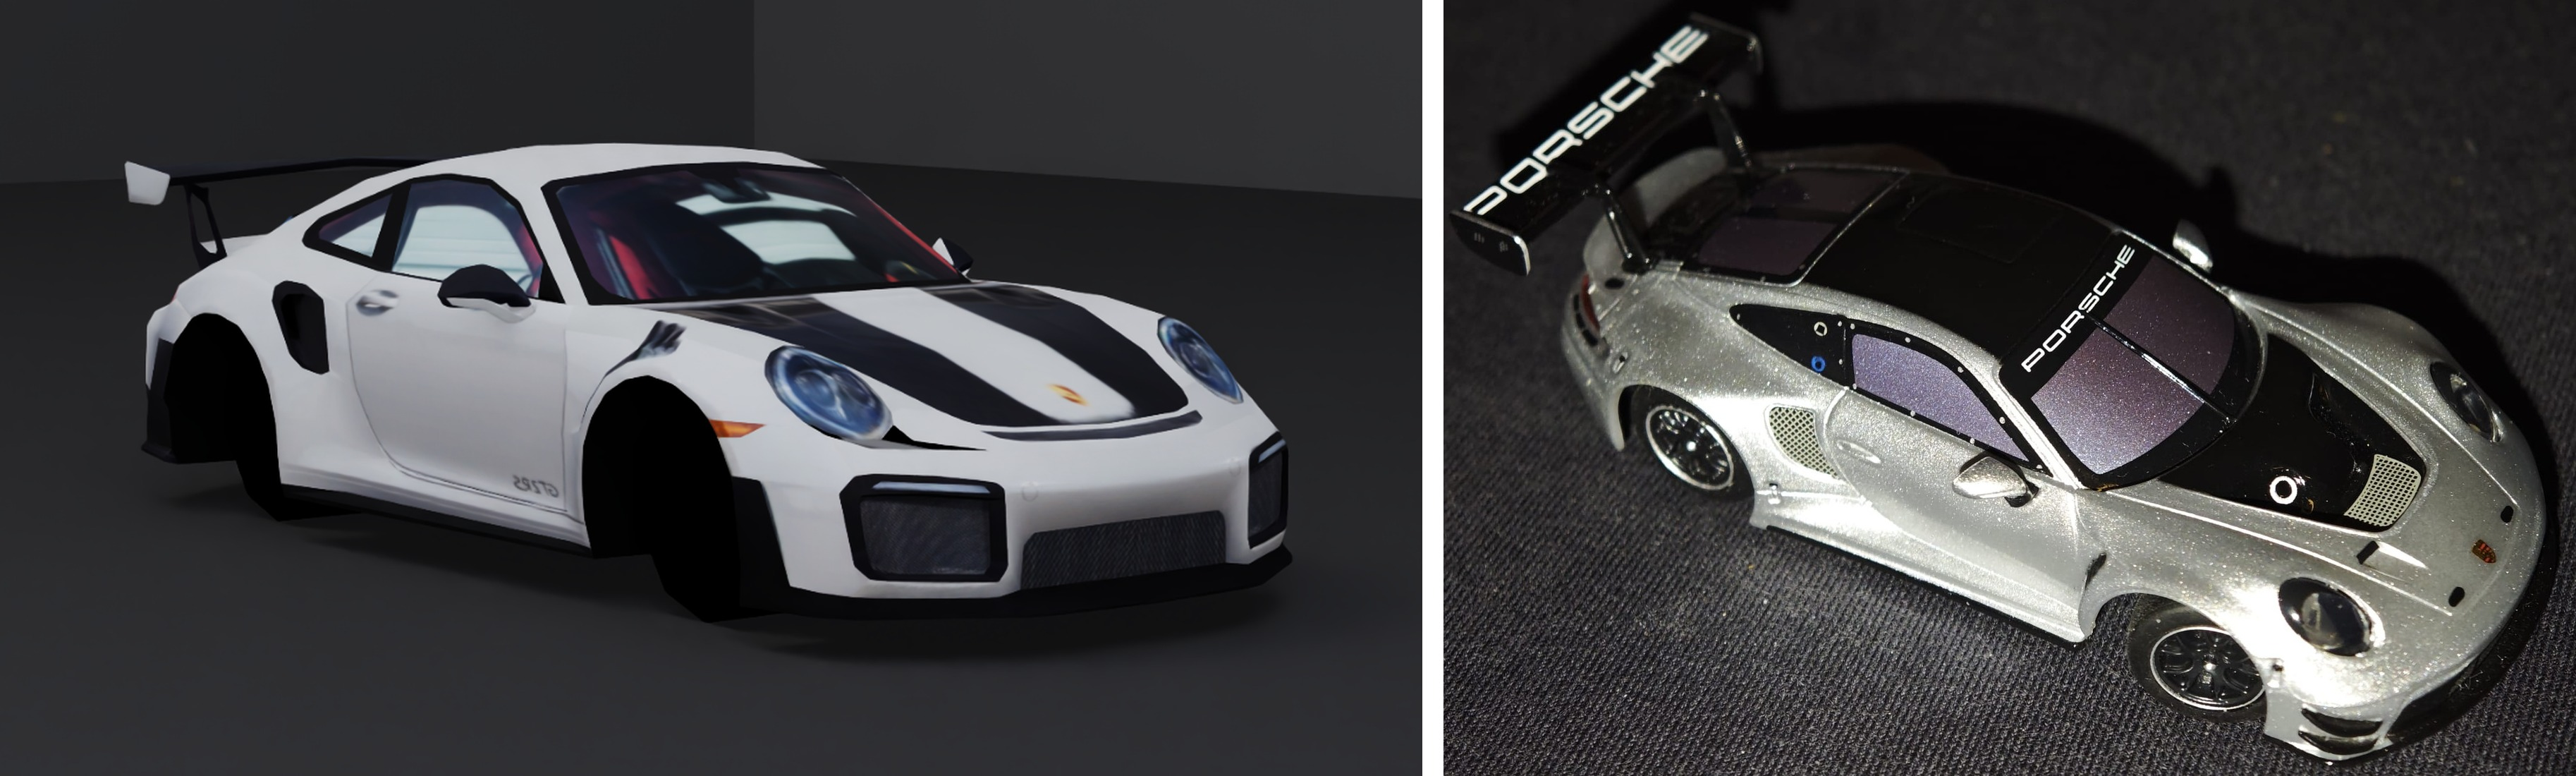
\includegraphics[width=\linewidth]{chapters/felix_teil/bilder/fahrzeug_modell_und_real.jpg}
  \caption{Sichtbares Fahrzeugmodell in Isaac Sim (links, Porsche 911 GT2 RS Weissach) und reales Fahrzeug der Carrera-Hybrid-Bahn (rechts, Porsche 991 GT3 R).}
  \label{fig:3d_fahrzeug}
\end{figure}

Das Kollisionsmodell des Autos ist weiterhin ein Quader mit vier Zylindern. Die Maße des Quaders und der Karosserie wurden jedoch am realen Carrera-Hybrid-Auto gemessen, damit Masse, Schwerpunktlage und Radaufstandspunkte mit der Realität übereinstimmen (Tabelle~\ref{tab:3d_fahrzeugdaten}); die Trägheitsmomente berechnet die Physik-Engine PhysX aus Masse und Form. Masse, Schwerpunkt und Reifenreibung beeinflussen, wie stark das Fahrzeug in Kurven schiebt oder ausbricht. Daher wurden sie so genau wie möglich übernommen.

\begin{table}[htbp]
  \centering
  \caption{Gemessene Fahrzeugdaten im Kollisionsmodell.}
  \label{tab:3d_fahrzeugdaten}
  \small
  \begin{tabular}{@{}l l@{}}
    \toprule
    \textbf{Größe} & \textbf{Wert} \\
    \midrule
    Länge $\times$ Breite $\times$ Höhe der Karosserie & \num{92.5} $\times$ \num{38.4} $\times$ \SI{21.5}{\milli\meter} \\
    Radstand                          & \SI{49.65}{\milli\meter} \\
    Spurweite vorne / hinten          & \SI{26.0}{\milli\meter} / \SI{24.5}{\milli\meter} \\
    Raddurchmesser vorne / hinten     & \SI{13.5}{\milli\meter} / \SI{14.0}{\milli\meter} \\
    Bodenfreiheit                     & \SI{1.85}{\milli\meter} \\
    Schwerpunkt                       & \SI{3.75}{\milli\meter} hinter der Fahrzeugmitte, \SI{10.1}{\milli\meter} über dem Boden \\
    Gesamtmasse                       & \SI{28.8}{\gram} \\
    Haftreibung Reifen vorne / hinten & \num{0.9} / \num{1.0} \\
    \bottomrule
  \end{tabular}
\end{table}

Die Lackierung des sichtbaren Modells (eine Textur der Karosserie) lag während aller hier beschriebenen Trainings nicht vor, der Agent hat das Fahrzeug nur als einfarbige Form gesehen (Abbildung~\ref{fig:3d_lackierung}). Darauf gehen die Einschränkungen in Abschnitt~\ref{sec:fazit_phase2} ein.

\begin{figure}[htbp]
  \centering
  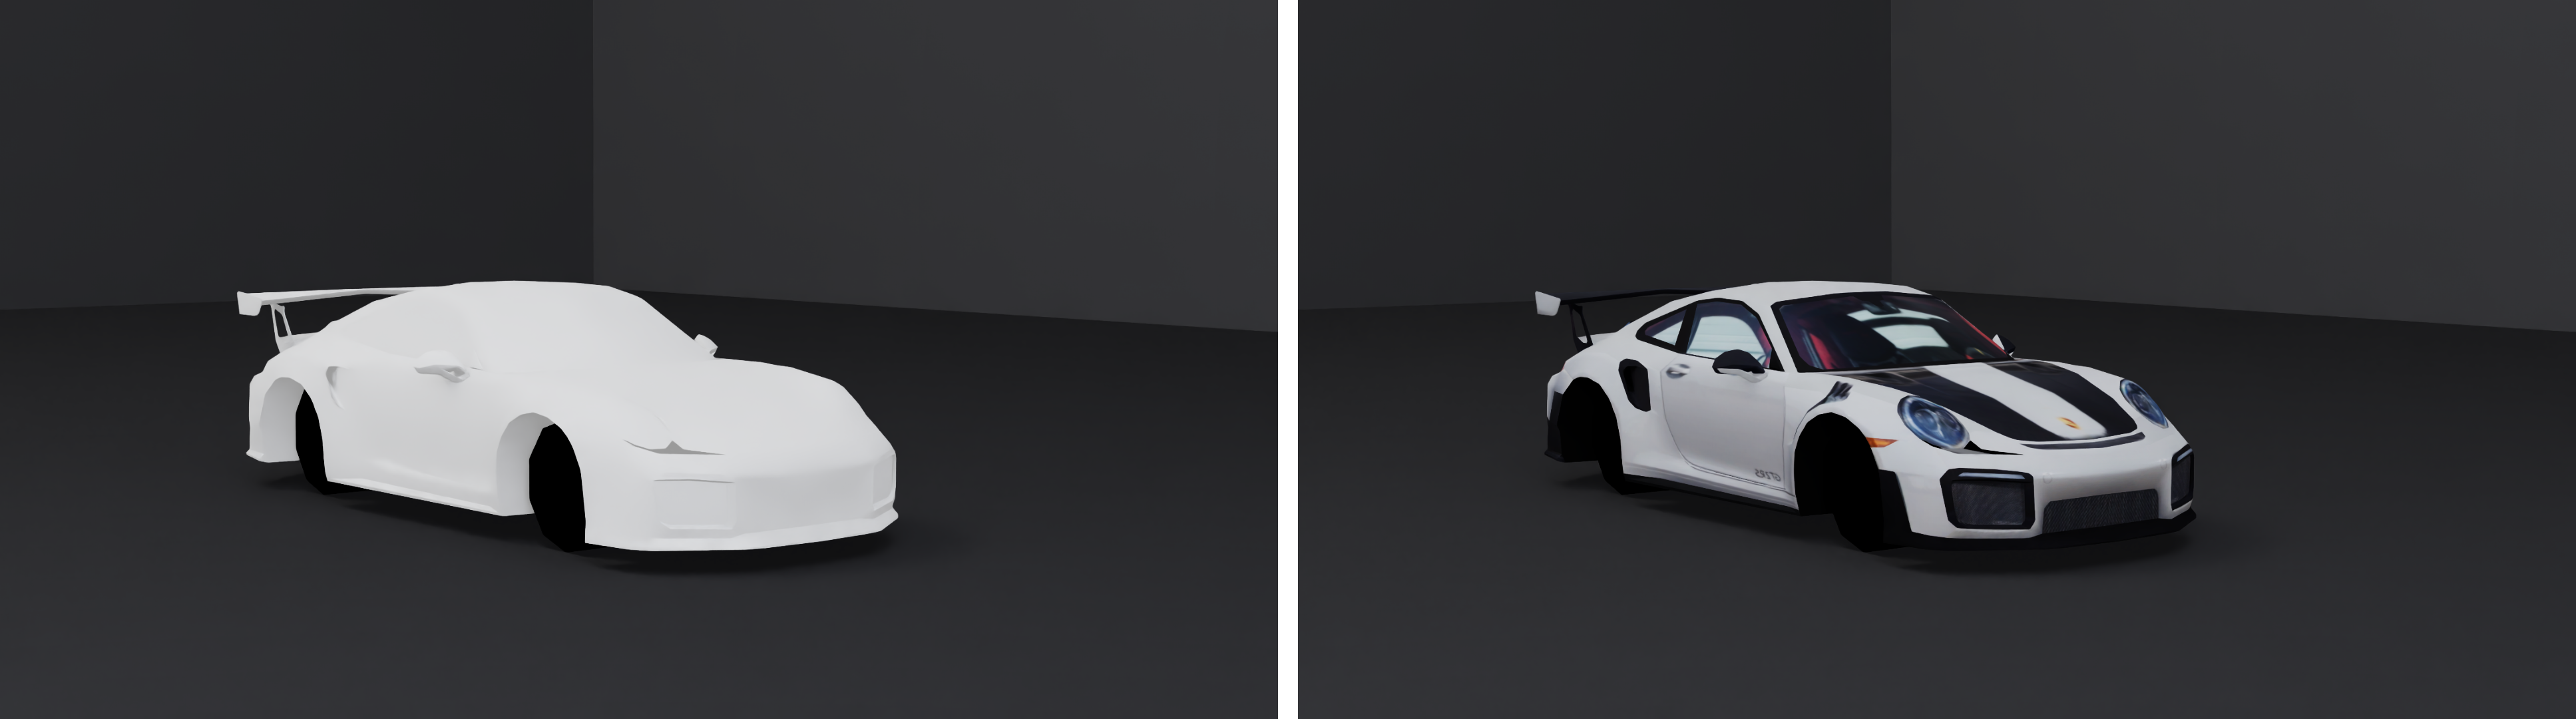
\includegraphics[width=\linewidth]{chapters/felix_teil/bilder/fahrzeug_ohne_mit_lackierung.png}
  \caption{Fahrzeugmodell ohne Lackierung, wie es der Agent im Training gesehen hat (links), und mit Lackierung (rechts).}
  \label{fig:3d_lackierung}
\end{figure}

\subsubsection{Antrieb und Fahrverhalten}
\label{subsec:3d_antrieb}

Anfangs beschleunigt und bremst das simulierte Fahrzeug sehr ruckartig und die Lenkung ist sehr direkt. Das reale Fahrzeug reagiert dagegen träge, da seine Elektronik das Fahrverhalten eines echten Autos nachbildet. Für den Längsantrieb wird deshalb das gemessene Modell aus Phase~1 unverändert übernommen (Gleichung~\eqref{eq:measured_v2}). Die Lenkung ist auf einen Einschlag von \SI{28.6}{\degree} begrenzt, was annähernd den \SI{30}{\degree} der 2D-Umgebung entspricht.

Das Auto wird über drei Werte gesteuert, für Gas und Bremse im Bereich 0 bis 1 und für die Lenkung von $-1$ bis 1. Gas und Bremse sind dabei den analogen Pedalen eines Controllers nachempfunden, die Lenkung dem Analogstick. Werden beide Pedale gleichzeitig betätigt, wirkt nur das stärkere. Darin weicht die 3D-Umgebung von Phase~1 ab, in der sich Gas und Bremse überlagern (vgl.\ Abschnitt~\ref{sec:ausblick}).

\subsubsection{Strecke und Streckenbegrenzung}
\label{subsec:3d_strecke}

Als Strecke wird während des Trainings zunächst dieselbe Streckenführung wie in der 2D-Umgebung verwendet. Da sie keine Höhenunterschiede hat, wird das Streckenbild als flache, texturierte Ebene in die Szene eingefügt.

Für das Reinforcement Learning muss jederzeit feststehen, wo sich das Fahrzeug auf der Strecke befindet. Dazu werden per Bildverarbeitung die Begrenzungslinien aus dem Streckenbild extrahiert, geglättet und als Linienzüge gespeichert. Daraus werden vier Bereiche abgeleitet:

\begin{itemize}
  \item die gültige Fahrbahn,
  \item die Randsteine links und rechts,
  \item der Bereich neben der Strecke,
  \item die Start- und Ziellinie.
\end{itemize}

Zur Kontrolle lassen sich die Linien in Isaac als dreidimensionale Wände anzeigen (Abbildung~\ref{fig:3d_grenzen_isaac}). Im Training werden sie nicht geladen.

\begin{figure}[htbp]
  \centering
  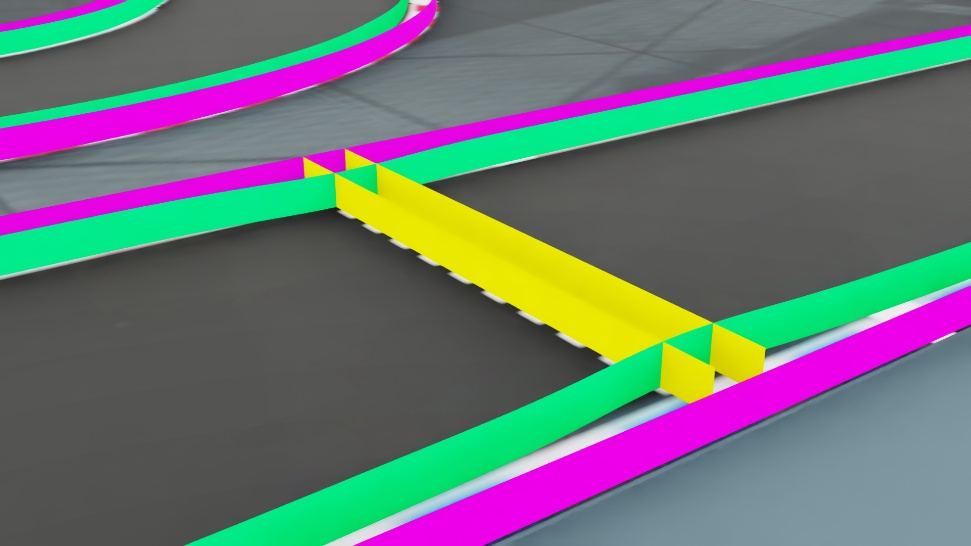
\includegraphics[width=0.8\linewidth]{chapters/felix_teil/bilder/grenzen_kontrollanzeige.jpg}
  \caption{Begrenzungslinien als Kontrollanzeige in Isaac Sim (grün: Fahrbahnkante, magenta: Außenkante der Randsteine, gelb: Start- und Ziellinie).}
  \label{fig:3d_grenzen_isaac}
\end{figure}

Ob das Auto die Strecke verlassen oder eine Runde beendet hat und wie weit es auf der Strecke vorangekommen ist, wird rein geometrisch berechnet. Für die äußeren Aufstandspunkte der Reifen wird geprüft, ob sie noch auf der gültigen Fahrbahn liegen. Liegt einer davon außerhalb, gilt das als Crash, und die Episode endet. Die Randsteine zählen dabei bereits als außerhalb. Eine Mittellinie dient als Bezug für den Fortschritt entlang der Strecke. Weiterhin ist auf den letzten \SI{0.9}{\meter} vor der Ziellinie eine Startzone definiert. Dort wird das Auto zu Beginn jeder Episode an einer zufälligen Stelle aufgestellt und bis zu \SI{5}{\centi\meter} seitlich zur Mittellinie versetzt (Abbildung~\ref{fig:3d_strecke_grenzen}).

\begin{figure}[htbp]
  \centering
  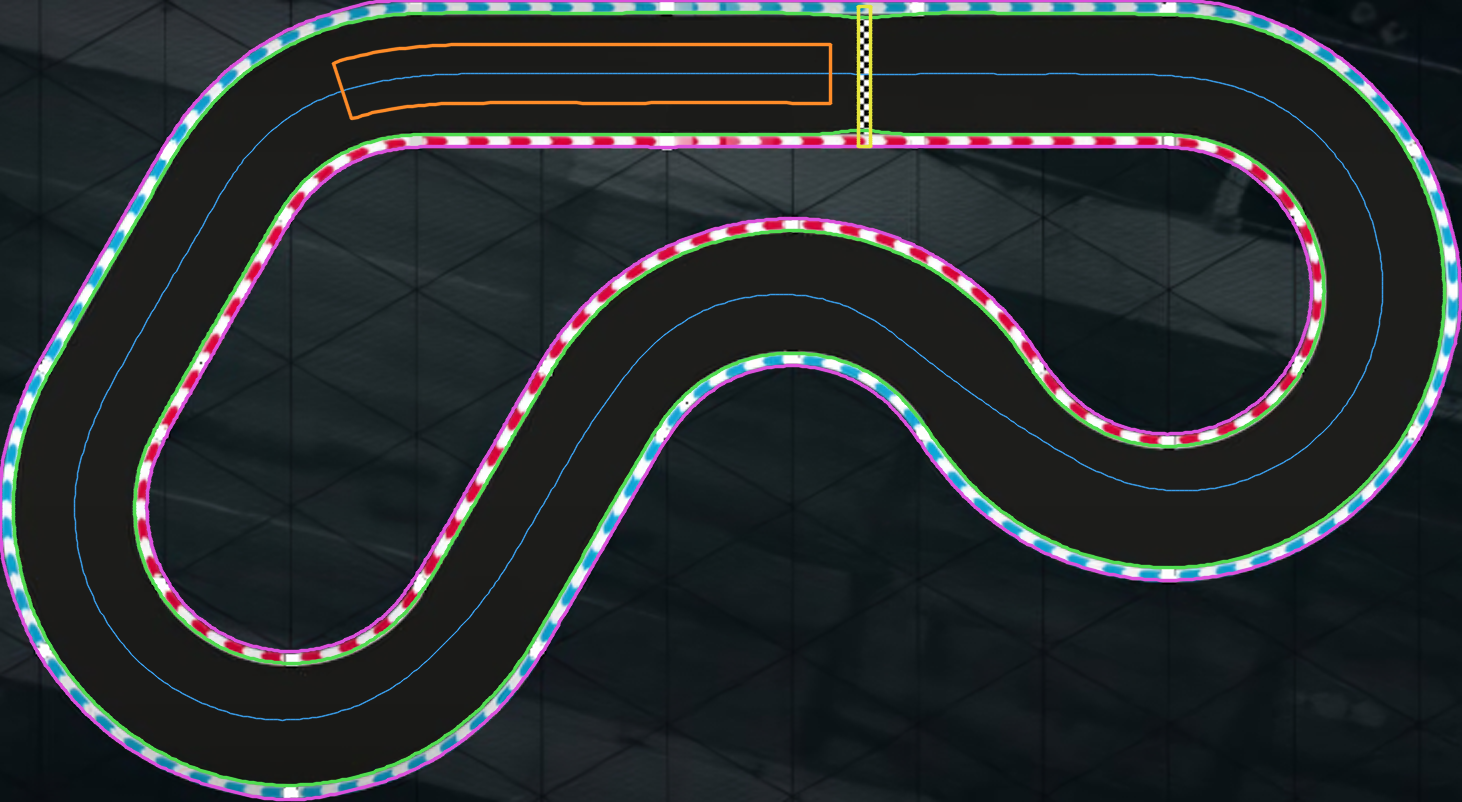
\includegraphics[width=\linewidth]{chapters/felix_teil/bilder/strecke_grenzen.png}
  \caption{Trainingsstrecke mit den abgeleiteten Grenzen. Grün: Fahrbahnkante; Magenta: Außenkante der Randsteine; Gelb: Start- und Ziellinie; Orange: Startzone; Blau: Mittellinie.}
  \label{fig:3d_strecke_grenzen}
\end{figure}

\subsubsection{Kamera und Beobachtung}
\label{subsec:3d_kamera}

Der Agent bekommt die Informationen der Umgebung über eine simulierte Kamera, deren Blickwinkel dem eines real umsetzbaren Aufbaus entspricht. Die Kamera hängt fest montiert \SI{3.05}{\meter} über der Mitte der Strecke und erfasst eine Fläche von \num{2.66} $\times$ \SI{1.60}{\meter}, also die gesamte Strecke. Wie in Phase~1 wird das Bild auf \num{250} $\times$ \num{150} Pixel verkleinert und in Graustufen umgerechnet. Die Beobachtung besteht analog zu Phase~1 aus den letzten drei Bildern als Stapel (Abschnitt~\ref{subsec:framestack}).

Ein Pixel deckt damit \SI{1.06}{\centi\meter} der Strecke ab (\SI{93.9}{\px\per\meter}), das Fahrzeug ist im Bild etwa \num{9} $\times$ \num{4} Pixel groß, gegenüber \num{7} $\times$ \num{3} Pixeln in Phase~1 bei gleicher Auflösung. Nach der Wahrnehmungsschwelle aus Phase~1 (Gleichung~\eqref{eq:schwelle}) muss sich das Fahrzeug zwischen zwei Bildern um mindestens einen Pixel bewegen, damit der Agent seine Bewegung im Bildstapel erkennen kann. Bei 30 Bildern je Sekunde liegt diese Schwelle hier bei \SI{0.32}{\meter\per\second}, in Phase~1 bei \SI{0.42}{\meter\per\second}. Die fahrenden Agenten bewegen sich mit \SIrange{0.53}{0.65}{\meter\per\second}, also \num{1.7} bis \num{2.0} Pixel je Bild, und damit deutlich oberhalb der Schwelle.

\subsubsection{Belohnung und Episodenende}
\label{subsec:3d_belohnung}

Die Belohnungsfunktion (\texttt{v3\_rundenzeit}) wird unverändert aus Phase~1 übernommen (Gleichung~\eqref{eq:reward}, Tabelle~\ref{tab:reward_gewichte}) und wie dort aus den exakten Zuständen der Simulation berechnet, nicht aus dem Kamerabild. Neu ist nur ein Term für den Fortschritt entlang der Strecke. Tabelle~\ref{tab:3d_belohnung} fasst die Terme zusammen.

\begin{table}[htbp]
  \centering
  \caption{Terme der Belohnung je Schritt.}
  \label{tab:3d_belohnung}
  \small
  \begin{tabularx}{\linewidth}{@{}l X l@{}}
    \toprule
    \textbf{Term} & \textbf{Wirkung} & \textbf{Gewicht} \\
    \midrule
    Geschwindigkeit         & $v^2 \cdot 2\,w_v$, belohnt schnelles Fahren & $w_v = 1$ \\
    Langsam-Gefälle         & lineare Strafe unter \SI{0.6}{\meter\per\second}, voll bei Stillstand & $w_{\text{slow}} = 4$ je Schritt \\
    Fortschritt (neu in 3D) & zurückgelegte Strecke entlang der Mittellinie & \num{50} je Meter \\
    Rundenbonus             & einmalig je vollständiger Runde & $+50$ \\
    Rundenzeit              & Verbesserung der eigenen Bestzeit, je eingesparten Schritt & \num{5} \\
    Lenkglättung            & Strafe je Lenkbewegung & \num{0.5} \\
    Falsche Richtung        & Grundstrafe je Schritt & $-30$ \\
    Crash                   & ersetzt alle anderen Terme, Episode endet & $-300$ \\
    \bottomrule
  \end{tabularx}
\end{table}

Eine Episode endet nach \num{2000} Schritten (\SI{66.67}{\second}), wenn das Auto die Fahrbahn verlässt (Crash) oder wenn die aufsummierte Belohnung unter $-3000$ fällt. Anschließend wird das Auto an einer neuen zufälligen Position in der Startzone aufgestellt.

\subsection{Vergleich zur 2D-Python-Umgebung}
\label{sec:3d_vergleich2d}

Dieser Abschnitt fasst zusammen, welche Bestandteile der 2D-Umgebung unverändert in die 3D-Umgebung übernommen werden und welche angepasst werden.

\subsubsection{Was übernommen und geändert wird}
\label{subsec:3d_uebernommen_geaendert}

Tabelle~\ref{tab:3d_vergleich2d} stellt die 2D-Umgebung aus Phase~1 und die 3D-Umgebung gegenüber. Die meisten Bestandteile werden unverändert übernommen; die Unterschiede ergeben sich vor allem aus der physikalischen Simulation, dem gerenderten Bild und den parallelen Umgebungen.

\begin{table}[!ht]
  \centering
  \caption{Bestandteile der 2D-Umgebung aus Phase~1 und der 3D-Umgebung im Vergleich.}
  \label{tab:3d_vergleich2d}
  \small
  \begin{tabularx}{\linewidth}{@{}>{\raggedright\arraybackslash}p{0.2\linewidth} >{\raggedright\arraybackslash}X >{\raggedright\arraybackslash}X@{}}
    \toprule
    \textbf{Bestandteil} & \textbf{Phase~1 (2D)} & \textbf{3D (Isaac)} \\
    \midrule
    Simulation                & kinematisches Modell in Python & Physik-Engine PhysX mit gemessenen Fahrzeugdaten \\
    Bild                      & gezeichnetes 2D-Bild & gerenderte 3D-Szene mit Licht und Schatten \\
    Beobachtung               & 3 Bilder à \num{250} $\times$ \num{150} Pixel, 4 Graustufen & übernommen; Agent~1 mit 256 Graustufen \\
    Längsdynamik              & gemessenes Antriebsmodell & übernommen \\
    Pedale                    & Gas und Bremse überlagern sich & nur das stärkere Pedal wirkt \\
    Streckengrenzen           & Polygonüberschneidung & geometrische Prüfung der Reifenaufstandspunkte \\
    Belohnung                 & \texttt{v3\_rundenzeit} & übernommen, ergänzt um den Fortschrittsterm \\
    Episoden                  & \num{2000} Schritte, Abbruch unter $-3000$, zufällige Startpositionen & übernommen \\
    Lernverfahren             & \ac{SAC} (Stable-Baselines3 \cite{raffin2021stable}), NatureCNN, Lernrate \num{5e-5}, $\gamma = \num{0.99}$, \num{0.5} Updates je Übergang & übernommen \\
    Erfahrungsspeicher        & jedes Bild einmal abgelegt, Stapel beim Ziehen & übernommen; bei Agent~2 mit \SI{2}{\bit} je Pixel \\
    Parallele Umgebungen      & eine & 4 (Agent~1) bzw.\ 16 (Agent~2) \\
    Lehrer                    & Lidar-Strahlen & exakter Zustand aus der Simulation \\
    Datenaufzeichnung         & mit injiziertem Rauschen & deterministisch \\
    Vortraining               & Nachahmen der Lehreraktionen & Agent~1 wie Phase~1; Agent~2 auf die Lage des Fahrzeugs \\
    Encoder zu Beginn des \ac{RL}-Trainings & lernt sofort mit & eingefroren \\
    Darstellung der Strecke   & eine & Agent~2: zwölf Darstellungen und Bildstörungen \\
    \bottomrule
  \end{tabularx}
\end{table}

\FloatBarrier

\subsubsection{Parallele Umgebungen und Erfahrungsspeicher}
\label{subsec:3d_parallel}

Der größte technische Unterschied zwischen der Python-Umgebung und Isaac Lab ist die Parallelisierung der Umgebungen. In Isaac dauert ein Simulationsschritt mit gerendertem Kamerabild rund \SI{96}{\milli\second}. Jede weitere parallele Umgebung verlängert diesen Schritt jedoch kaum, da Isaac die Physik aller Umgebungen gemeinsam berechnet und alle Kamerabilder in einem Aufruf rendert: Vier Umgebungen benötigen nur \SI{4}{\percent} mehr Zeit als eine, 16 Umgebungen rund \SI{14}{\percent} mehr (\SI{109}{\milli\second}).

\paragraph{Schritt und Übergang.}
Mit parallelen Umgebungen muss zwischen Schritt und Übergang unterschieden werden. Ein Schritt ist ein Simulationsschritt von $\tfrac{1}{30}$\,\si{\second}; ein Übergang ist ein einzelnes Erfahrungstupel aus Beobachtung, Aktion, Belohnung und Folgebeobachtung einer Umgebung (Abschnitt~\ref{subsec:replay}). Bei 16 Umgebungen entstehen je Schritt 16 Übergänge. Trainingslängen werden im Folgenden in Übergängen angegeben, Episodenlängen in Schritten.

\paragraph{Lernen und Erfahrungsspeicher.}
Mehr Umgebungen beschleunigen jedoch nur das Sammeln von Erfahrung, nicht das Lernen. Damit das Verhältnis von \num{0.5} Updates je Übergang aus Phase~1 erhalten bleibt, muss die Zahl der Updates mit der Zahl der Umgebungen wachsen, und ein Update dauert mit rund \SI{168}{\milli\second} länger als ein Simulationsschritt. Außerdem teilt Stable-Baselines3 den Replay-Buffer gleichmäßig auf die Umgebungen auf.

% 06-trainingsablauf.tex
\section{Trainingsablauf in Isaac}
\label{sec:trainingsablauf}

Wie in Phase~1 gezeigt, ist es von Vorteil, das \ac{RL}-Training nicht ohne Vorbereitung zu starten. Ein Kamera-Agent, der von Null an lernt, muss zwei Dinge gleichzeitig herausfinden: was die Pixel bedeuten und wie man fährt. Das einzige Signal dafür ist die Belohnung. Um das zu erleichtern, wird der Bildteil des Netzes vorab überwacht trainiert. Anschließend folgen die beiden fahrenden Kamera-Agenten, die im Verlauf der Arbeit entstanden sind, im Folgenden Agent~1 und Agent~2. Beide durchlaufen dieselben vier Stufen, unterscheiden sich aber im Ziel des Vortrainings und in den Darstellungen der Strecke: Agent~1 lernt auf einer einzigen Darstellung, Agent~2 auf zwölf.

\subsection{Die Trainingspipeline in 3D}
\label{sec:pipeline3d}

Entsprechend der Python-Umgebung wird auch hier eine mehrstufige Trainingspipeline verwendet, um den Ablauf des \ac{RL}-Trainings effizienter zu gestalten. Diese Pipeline besteht aus vier separaten Stufen, wie in Abbildung~\ref{fig:pipeline_stufen} zu sehen.

\begin{figure}[htbp]
  \centering
  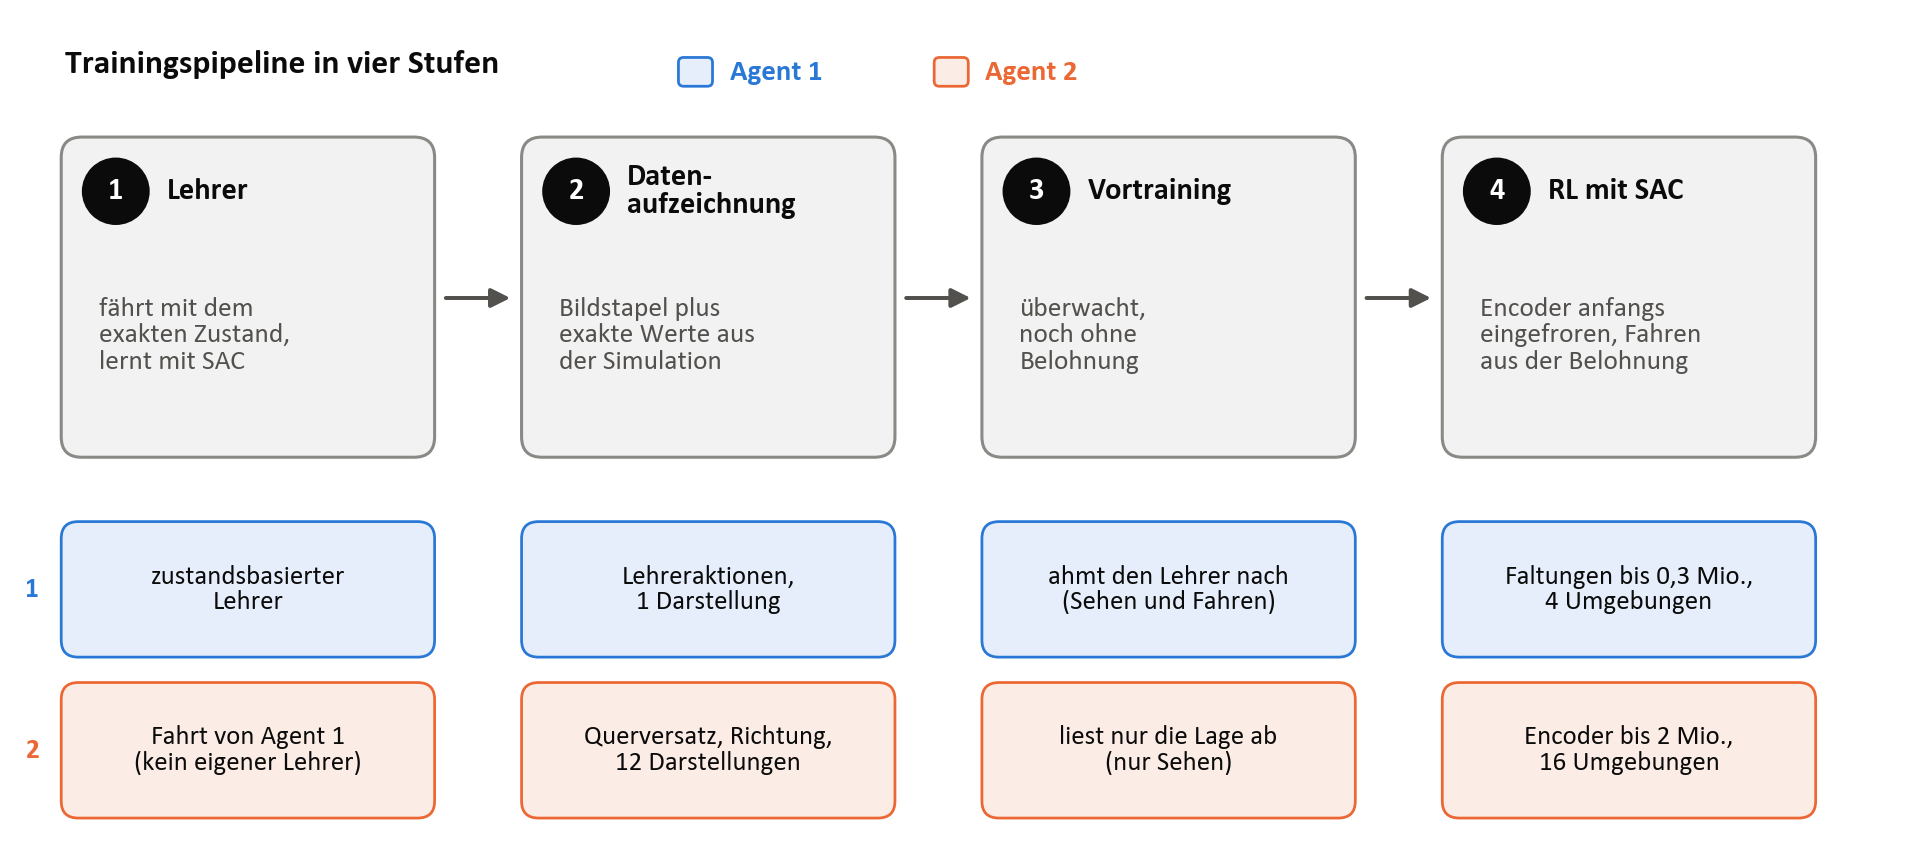
\includegraphics[width=\linewidth]{chapters/felix_teil/bilder/pipeline_stufen.png}
  \caption{Trainingspipeline in vier Stufen. Oben der gemeinsame Ablauf, darunter die Unterschiede zwischen Agent~1 (blau) und Agent~2 (orange).}
  \label{fig:pipeline_stufen}
\end{figure}

\paragraph{Stufe 1 -- Lehrer.}
Wie in Phase~1 wird zuerst ein Agent trainiert, der als Lehrer für den späteren bildbasierten Agenten dient (Abschnitt~\ref{subsec:privileged}). Während der Lehrer in der 2D-Umgebung anhand von Lidar-Strahlen lernte, ist er hier zustandsbasiert. Er erhält den exakten Zustand aus der Simulation, also Geschwindigkeit, Drehrate, Richtungsfehler, Querversatz und die Abstände zu beiden Fahrbahnkanten, sowie seine letzte Aktion. Da Isaac alle diese Größen ohnehin kennt, ist es nicht nötig, Abstandsstrahlen nachzubilden.

Dieser Lehrer wird mit \ac{SAC} auf 64 parallelen Umgebungen trainiert und fährt nach \num{768000} Übergängen 8 Runden je Episode ohne Crash, mit einer Rundenzeit von ca.\ \SI{8.3}{\second}. Damit ist gezeigt, dass Physik und Belohnungsfunktion in 3D lösbar sind.

\paragraph{Stufe 2 -- Datenaufzeichnung.}
Anschließend fährt der Lehrer in der Kamera-Umgebung. Zu jedem Schritt werden der Bildstapel und die Aktion des Lehrers gespeichert, insgesamt \num{48000} Paare. Abweichend von Phase~1 fährt der Lehrer dabei deterministisch, ohne injiziertes Rauschen (Gleichung~\eqref{eq:noise}), Vielfalt im Datensatz entsteht nur durch die zufälligen Startpositionen. Für Agent~2 stammen die Bilder stattdessen aus einer Fahrt von Agent~1, die in allen zwölf Darstellungen der Strecke gerendert wird (Abschnitt~\ref{sec:agent2}).

\paragraph{Stufe 3 -- Vortraining.}
Vortrainiert wird der Teil des Netzes, der aus dem Bildstapel Merkmale berechnet, im Folgenden Merkmalsextraktor (Encoder). Er besteht wie in Phase~1 aus den drei Faltungsschichten des NatureCNN \cite{mnih2015human} und einer voll verbundenen Schicht mit 512 Neuronen. Für Agent~1 lernt das Netz analog zu Phase~1, die Aktionen des Lehrers nachzuahmen (\ac{BC}, Abschnitt~\ref{subsec:il}). Bestätigt wurde dabei die Warnung aus Abschnitt~\ref{sec:ergebnisse_pipeline}, dass ein niedriger Vorhersagefehler kein Fahrkönnen belegt: Von zwei Netzen fuhr das mit dem schlechteren Fehler ($R^2 = \num{0.25}$ gegen \num{0.47}) \SI{60}{\percent} weiter. Nach dem Vorhersagefehler wäre das schlechtere Netz ausgewählt worden. Vortrainierte Netze wurden deshalb im Fahrversuch bewertet, nicht am Verlust.

Für Agent~2 lernt der Encoder dagegen nicht die Aktionen, sondern nur die Lage des Fahrzeugs, Querversatz zur Mittellinie und Richtungsfehler, beide aus der Simulation exakt bekannt. Vortrainiert wird damit nur das Sehen, nicht das Fahren, wie auf eine Situation zu reagieren ist, lernt der Agent erst im \ac{RL}-Training.

\paragraph{Stufe 4 -- Online-Training mit SAC.}
Die vortrainierten Gewichte werden in das Netz des \ac{RL}-Agenten übertragen und als Grundlage für das \ac{SAC}-Training verwendet. Für Agent~1 werden nur die Faltungsschichten übernommen, für Agent~2 der gesamte Encoder. Der Kopf hinter dem Encoder, der aus den Merkmalen die Aktionen und ihre Bewertung berechnet, ist zu Beginn zufällig initialisiert.

Gerade am Anfang des Trainings sind die Gradienten des Reinforcement Learning stark verrauscht, der Agent verlässt nach wenigen Schritten die Fahrbahn, und der Critic kann den Wert einer Aktion kaum einschätzen. Lernt der Encoder in dieser Phase mit, überschreiben diese Gradienten das vortrainierte Sehen, bevor der Kopf gelernt hat, es zu nutzen.

Der Encoder wird deshalb zu Beginn eingefroren: Seine Gewichte bleiben für eine festgelegte Zahl von Übergängen unverändert, und nur der Kopf lernt. Danach wird der Encoder aufgetaut und lernt mit. Die Gradienten verfeinern das Sehen nun, statt es zu zerstören. Bei Agent~1 waren die Faltungsschichten bis \num{0.3}~Mio.\ Übergänge eingefroren, bei Agent~2 der gesamte Encoder bis 2~Mio. Wie entscheidend dieser Schritt ist, zeigt ein Gegenversuch (Abschnitt~\ref{sec:einfrieren}).

\subsection{Training des Kamera-Agenten}
\label{sec:kamera_training}

Der Kamera-Agent wird, wie in Phase~1 erarbeitet, mit \ac{SAC} trainiert (Abschnitte~\ref{subsec:ppo_sac} und~\ref{subsec:ppo_sac_vergleich}); auch die Netzarchitektur, das NatureCNN, stammt aus Phase~1. Actor und Critic besitzen jeweils einen eigenen Encoder, dahinter je einen Kopf, der die drei Aktionen bzw.\ deren Bewertung berechnet.

Während des Trainings fährt der Agent parallel in mehreren Umgebungen. Jeder Übergang landet im Erfahrungsspeicher, aus dem nach jedem Simulationsschritt Stichproben für die Updates gezogen werden. Die Aktionen sind dabei zufällig gestreut, damit der Agent erkundet.

Als Eingabe erhält der Agent ausschließlich den Bildstapel. Belohnung, frühere Aktionen oder die Geschwindigkeit werden nicht zurückgeführt, die Belohnung dient nur als Lernsignal für den Critic.

\paragraph{Bewertung.}
Die Agenten werden nach dem Training deterministisch bewertet, also ohne Zufallsanteil der Aktionen und ohne Bildstörungen, mit zufälligen Startpositionen und getrennt je Darstellung der Strecke. Dabei werden Runden je Episode, mittleres Tempo, beste Rundenzeit und der Anteil der Episoden, die mit einem Crash enden, gemessen. Die Werte aus dem Training eignen sich dafür nicht, weil die Aktionen dort zufällig gestreut und über alle Darstellungen gemittelt sind. Da gute Agenten in \SI{66.67}{\second} das Zeitlimit von etwa sechs Runden erreichen, wurden die fertigen Modelle zusätzlich mit \SI{200}{\second} langen Episoden gemessen.

\subsection{Probleme auf dem Weg zum ersten Agenten}
\label{sec:probleme_agent1}

Bis zum ersten fahrenden Kamera-Agenten vergingen etwa \SI{125}{\hour} Rechenzeit in Läufen, die nichts lernen konnten. Die wesentlichen Fehler traten ohne Absturz oder Warnung auf. Mehrere Fehler betrafen die Vortrainingskette: invertierte Lehrerbilder, Lehreraktionen außerhalb des gültigen Wertebereichs und das Speichern der letzten statt der besten Trainingsepoche.

Auch mit korrektem Bild lernte der Agent zunächst nicht zu fahren. Zum einen bestand eine Belohnungsfalle: Ohne den Fortschrittsterm brachte Geradeausfahren erst ab \SI{0.52}{\meter\per\second} Pluspunkte, sodass ein schnelles Verlassen der Fahrbahn für den Agenten günstiger war als langsames Weiterfahren. Erst der Fortschrittsterm (Abschnitt~\ref{subsec:3d_belohnung}) beseitigte diese Falle. Zum anderen verlor der Agent seine vortrainierte Sehfähigkeit. Das vortrainierte Netz fuhr allein 120 Schritte weit, der Agent nach \num{762000} Übergängen nur noch 44 und damit kürzer als ein Fahrzeug, das ohne Lenken 86 Schritte weit fährt. Das \ac{RL} hatte die vortrainierten Merkmale überschrieben.

\subsection{Einfrieren des Encoders}
\label{sec:einfrieren}

Wie wichtig das Einfrieren des Encoders ist, zeigt ein Gegenversuch: zwei Läufe mit identischem Aufbau, einmal mit eingefrorenem Encoder bis 2~Mio.\ Übergänge und einmal ohne Einfrieren. Der Aufbau entspricht dem von Agent~2 (Abschnitt~\ref{sec:agent2}).

Neben der Episodenlänge werden dafür zwei Kennzahlen aufgezeichnet, beide auf einer Stichprobe von Bildern aus dem Erfahrungsspeicher. Die erste ist der Anteil inaktiver Neuronen der 512er-Schicht, also der Neuronen, die für alle Bilder der Stichprobe null ausgeben. Ein solches Neuron trägt keine Information über das Bild mehr, ist fast die gesamte Schicht inaktiv, erreicht den Kopf des Netzes kaum noch Bildinformation. Die zweite ist die Streuung des Lenkbefehls über die Bilder der Stichprobe. Ist sie null, gibt der Agent für jedes Bild denselben Lenkbefehl aus, er ist blind. In den üblichen Trainingskurven ist beides nicht zu erkennen, sie verlaufen lediglich flach. Tabelle~\ref{tab:gegenversuch_einfrieren} und Abbildung~\ref{fig:gegenversuch_einfrieren} zeigen den Verlauf.

\begin{table}[htbp]
  \centering
  \caption{Gegenversuch Einfrieren, Werte im Trainingsverlauf (Episodenlänge in Schritten / Anteil inaktiver Neuronen der 512er-Schicht / Streuung des Lenkbefehls).}
  \label{tab:gegenversuch_einfrieren}
  \small
  \begin{tabular}{@{}l c c@{}}
    \toprule
    \textbf{Übergänge} & \textbf{ohne Einfrieren} & \textbf{eingefroren bis 2~Mio.} \\
    \midrule
    \num{0.5}~Mio.  & 33 / \SI{89}{\percent} / \num{0.000}   & 42 / \SI{81}{\percent} / \num{0.99} \\
    \num{2.0}~Mio.  & 31 / \SI{92}{\percent} / \num{0.000}   & 58 / \SI{63}{\percent} / \num{0.91} \\
    \num{2.5}~Mio.  & 31 / \SI{96}{\percent} / \num{0.000}   & 270 / \SI{22}{\percent} / \num{1.49} \\
    \num{2.95}~Mio. & 31 / \SI{99.6}{\percent} / \num{0.000} & 444 / \SI{18}{\percent} / \num{1.42} \\
    \bottomrule
  \end{tabular}
\end{table}

\begin{figure}[htbp]
  \centering
  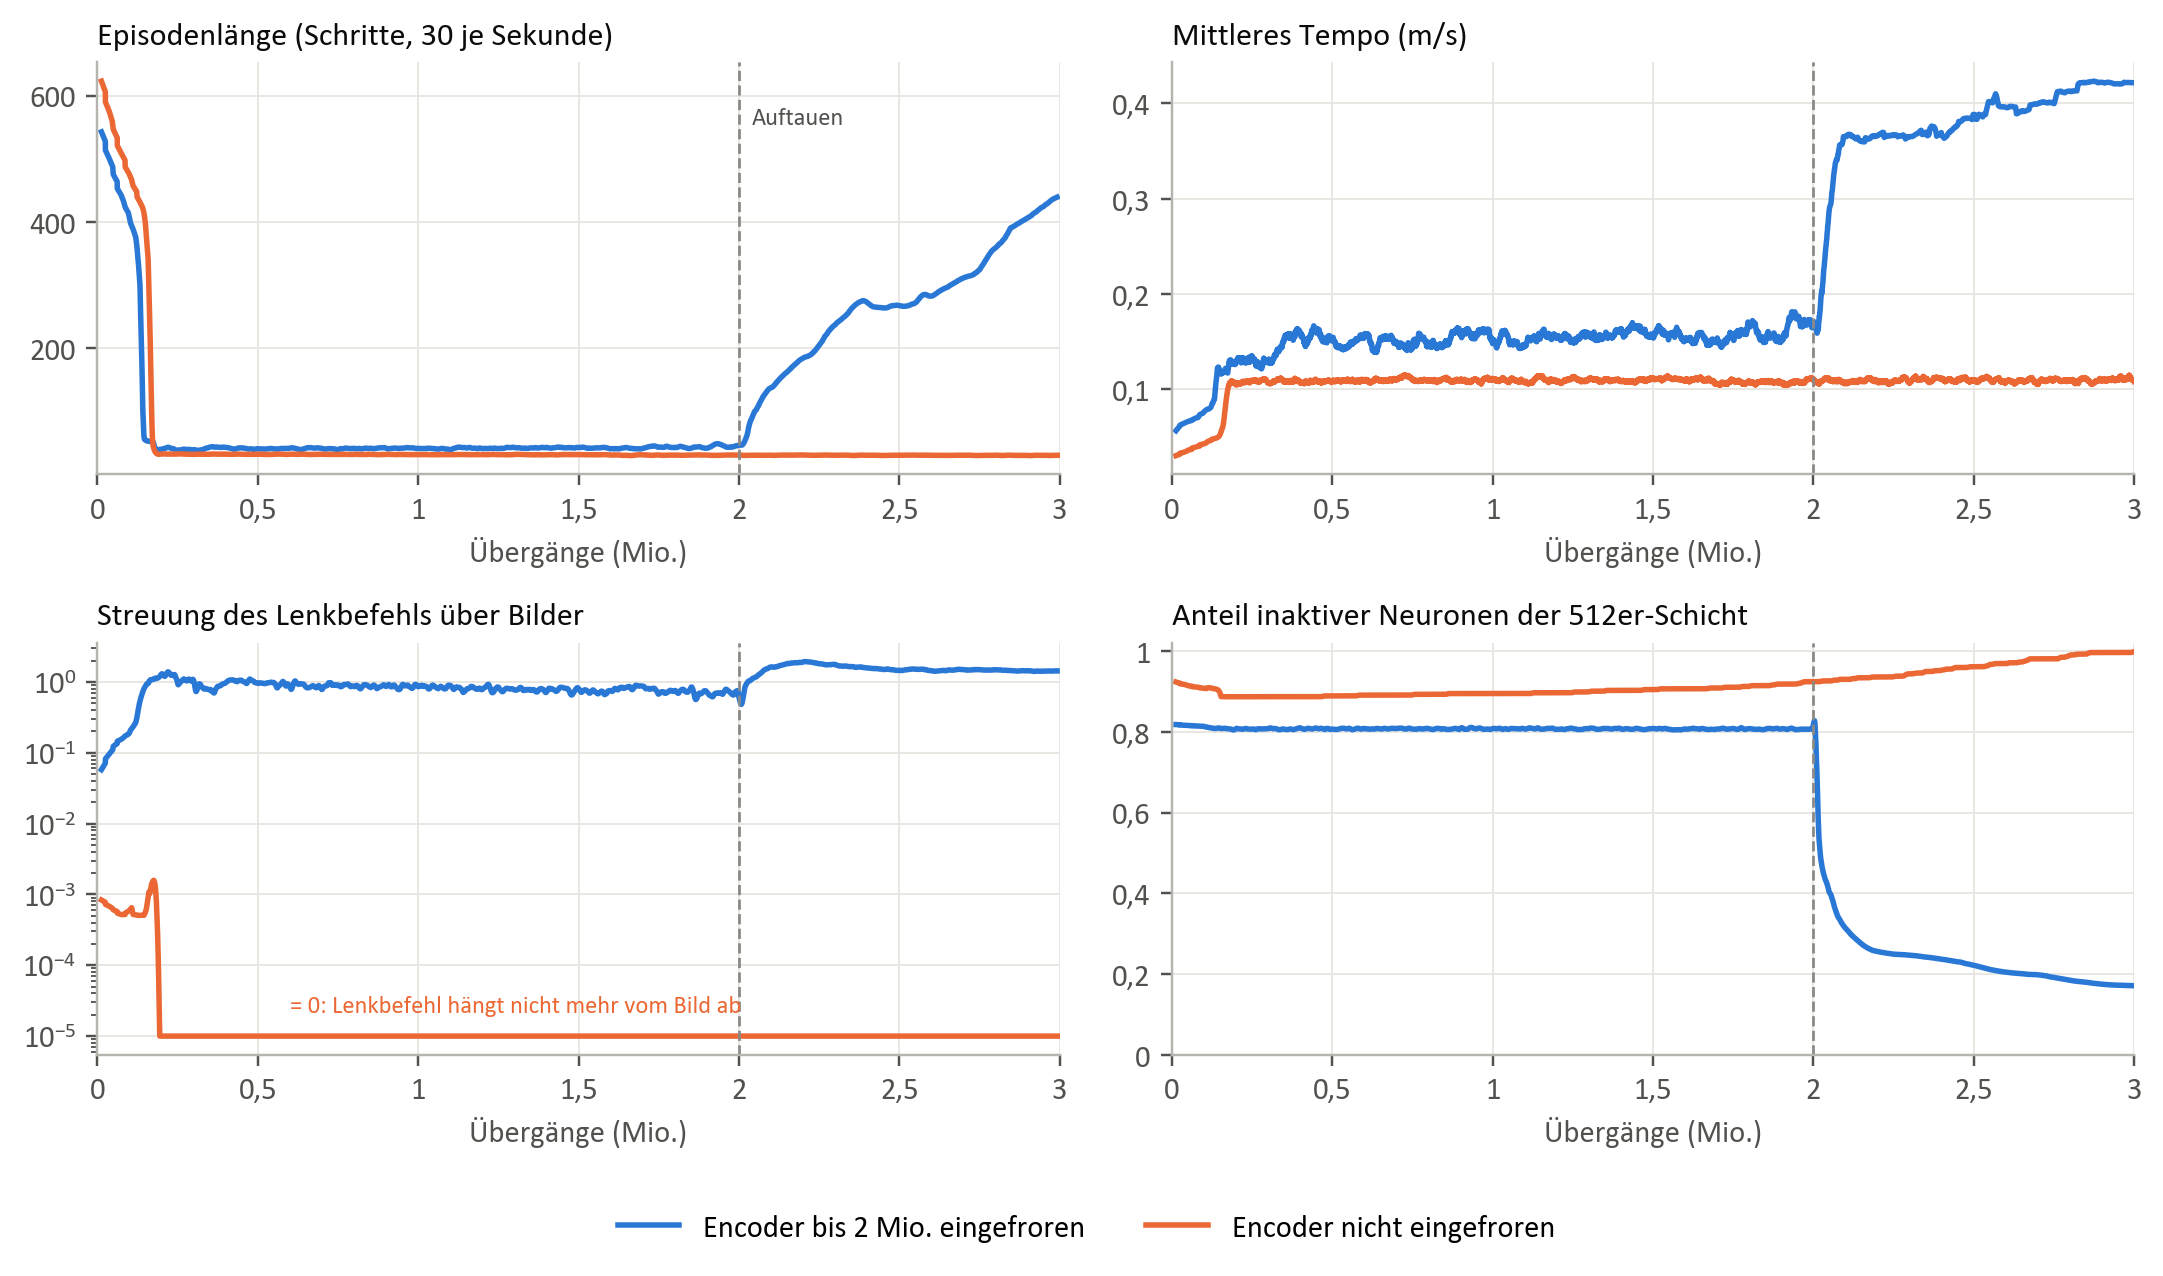
\includegraphics[width=\linewidth]{chapters/felix_teil/bilder/gegenversuch_einfrieren.png}
  \caption{Gegenversuch Einfrieren: identischer Aufbau mit eingefrorenem (blau) und nicht eingefrorenem Encoder (orange) auf \texttt{kurs\_A}.}
  \label{fig:gegenversuch_einfrieren}
\end{figure}

Ohne Einfrieren wird der Agent blind. Schon nach einer halben Million Übergängen hängt der Lenkbefehl nicht mehr vom Bild ab, und die 512er-Schicht stirbt bis zum Ende fast vollständig ab. Der Agent fährt keine Runde, die Episoden enden nach etwa einer Sekunde. Mit Einfrieren bleibt das Sehen erhalten; nach dem Auftauen steigen Episodenlänge und Tempo, und der Agent fährt nach \num{2.9}~Mio.\ Übergängen seine erste Runde.

Damit ist das Einfrieren als notwendig belegt. Ohne Schutz zerstört das \ac{RL} den vortrainierten Encoder in den ersten Hunderttausend Übergängen, bevor der Kopf gelernt hat, ihn zu nutzen.

\subsection{Der erste fahrende Kamera-Agent}
\label{sec:agent1}

Nach Behebung dieser Probleme gelingt mit Agent~1 das erste Training eines Kamera-Agenten, der zuverlässig Runden fährt.

\subsubsection{Genutzte Parameter}
\label{subsec:agent1_einstellungen}

Mit den Einstellungen aus Tabelle~\ref{tab:agent1_einstellungen} gelang das erste Training eines Kamera-Agenten, der zuverlässig Runden fährt.

Gegenüber den vorherigen Läufen wurden zwei Dinge geändert: Statt 64 laufen nur noch 4 parallele Umgebungen, wodurch der Erfahrungsspeicher je Umgebung 69 statt 4 Minuten Fahrt enthält, und die Faltungsschichten bleiben bis \num{0.3}~Mio.\ Übergänge eingefroren.

\begin{table}[htbp]
  \centering
  \caption{Einstellungen von Agent~1.}
  \label{tab:agent1_einstellungen}
  \small
  \begin{tabularx}{\linewidth}{@{}l X@{}}
    \toprule
    \textbf{Einstellung} & \textbf{Agent~1} \\
    \midrule
    Parallele Umgebungen                    & 4 \\
    Beobachtung                             & 3 Bilder à \num{250} $\times$ \num{150} Pixel, 256 Graustufen \\
    Darstellungen der Strecke               & 1 \\
    Vortraining                             & \ac{BC} auf \num{48000} Lehrerpaaren; übernommen: Faltungsschichten \\
    Eingefroren                             & Faltungsschichten bis \num{0.3}~Mio.\ Übergänge \\
    Batchgröße / Updates                    & 512 / 2 je Simulationsschritt (\num{0.5} je Übergang) \\
    Erfahrungsspeicher gesamt / je Umgebung & \num{500000} / \num{125000} Übergänge ($\approx$ \SI{69}{\minute} Fahrt) \\
    Lernrate / Diskontfaktor $\gamma$       & \num{5e-5} / \num{0.99} \\
    Episodenlänge                           & \SI{66.67}{\second}; in der Fortsetzung \SI{133.33}{\second} \\
    Übergänge im fertigen Modell            & \num{2.2}~Mio.\ (\num{1.2} + \num{1.0}) \\
    Durchsatz                               & $\approx$ 11 Übergänge/s (rund \SI{38}{\hour} je \num{1.5}~Mio.) \\
    \bottomrule
  \end{tabularx}
\end{table}

\subsubsection{Das Ergebnis}
\label{subsec:agent1_ergebnis}

Der erste erfolgreiche Agent fährt seine erste vollständige Runde nach rund \num{0.92}~Mio.\ Übergängen. Da das Training auf \num{1.5}~Mio.\ Übergänge ausgelegt ist und die Ergebnisse erstmals vielversprechend sind, wird es fortgesetzt: ausgehend vom Stand bei \num{1.2}~Mio.\ Übergängen um weitere \num{1.0}~Mio.\ Übergänge, mit doppelt so langen Episoden (\num{4000} statt \num{2000} Schritte). Längere Episoden setzen den Schwerpunkt auf stabiles Fahren, da der Agent mehr Runden am Stück fahren muss.

Dieser Agent lernt auf einer Strecke mit stets gleicher Darstellung. Abbildung~\ref{fig:agent1_verlauf} zeigt den Verlauf beider Trainingsabschnitte.

\begin{figure}[htbp]
  \centering
  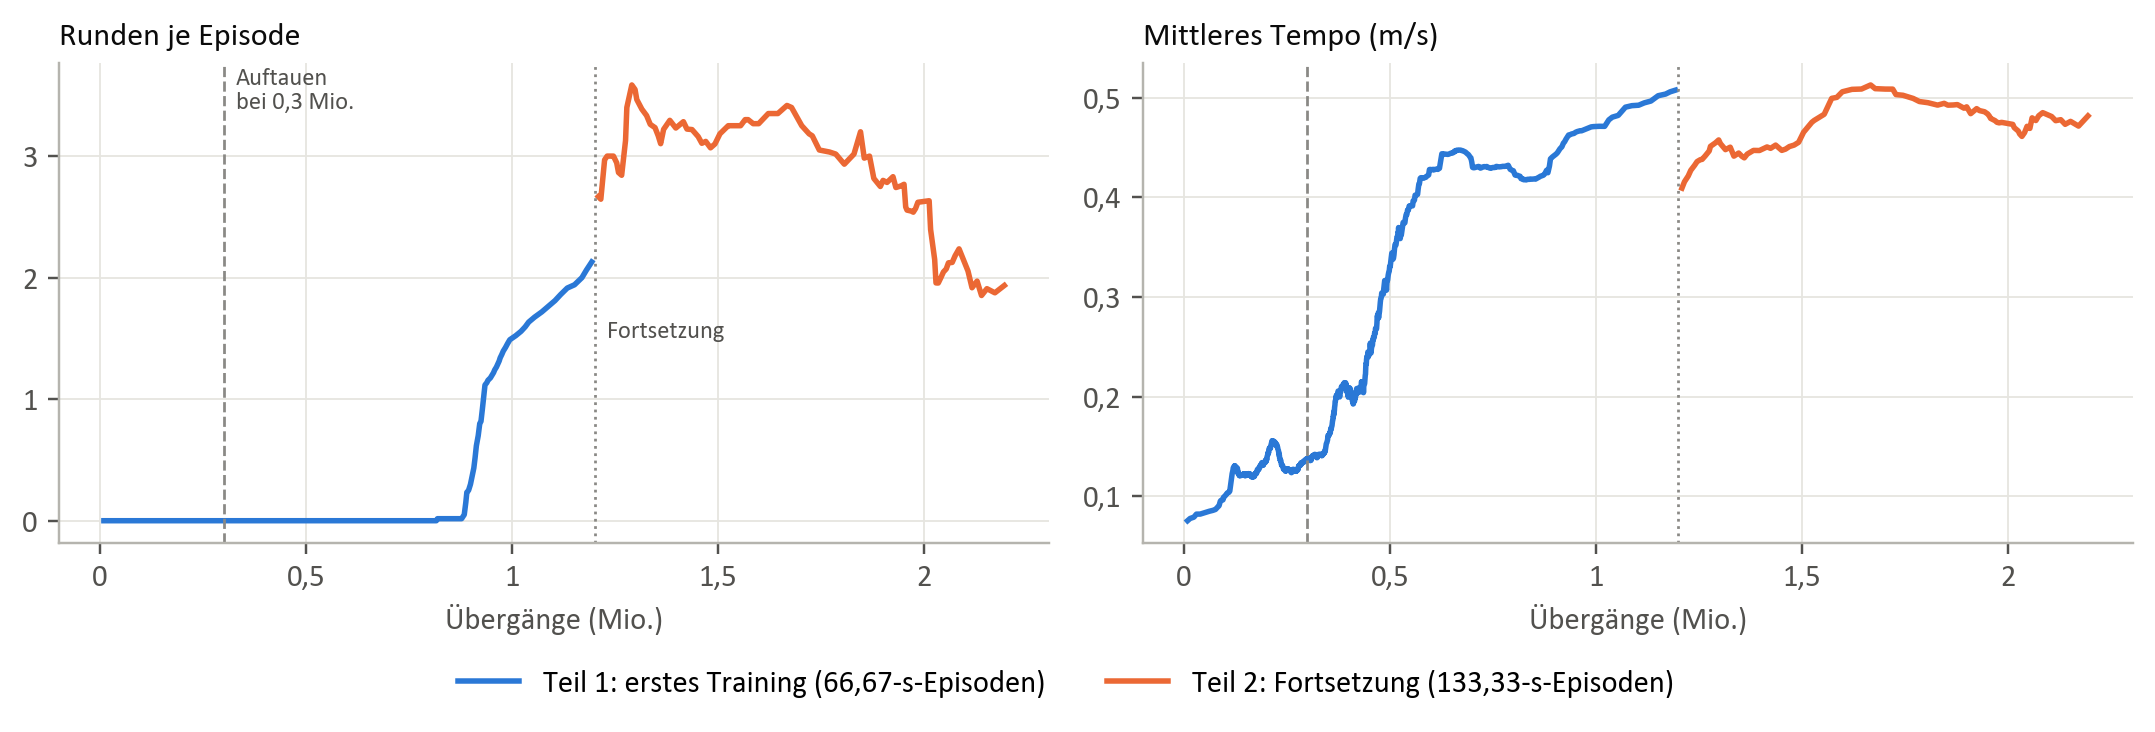
\includegraphics[width=\linewidth]{chapters/felix_teil/bilder/agent1_verlauf.png}
  \caption{Trainingsverlauf von Agent~1 (Werte mit Explorationsrauschen). Blau: erstes Training, orange: Fortsetzung mit doppelt so langen Episoden; gestrichelt: Auftauen der Faltungsschichten.}
  \label{fig:agent1_verlauf}
\end{figure}

Deterministisch gemessen, also ohne Explorationsrauschen und über zehn Episoden, fährt Agent~1 auf seiner Darstellung \num{6.4} Runden je Episode von \SI{66.67}{\second}, mit einer mittleren Geschwindigkeit von \SI{0.65}{\meter\per\second} und einer besten Runde von \SI{8.65}{\second}. Ca.\ \SI{10}{\percent} der Episoden enden mit einem Crash. Zum Vergleich fährt der zustandsbasierte Lehrer, der alle Größen exakt kennt, auf der gleichen Strecke etwa \SI{8.3}{\second} je Runde. Agent~1 ist also rund \SI{4}{\percent} langsamer, obwohl dieser die Lage und Bewegungen des Fahrzeugs aus \num{9} $\times$ \num{4} Pixeln ablesen muss. In Episoden von \SI{200}{\second} fährt er im Mittel \num{10.4} Runden mit einer besten Runde von \SI{8.59}{\second}. In 3 von 10 Episoden fährt er rund 20 Runden ohne Crash, \SI{70}{\percent} der langen Episoden enden jedoch vorzeitig. Der beste Bild-Agent der 2D-Umgebung schaffte unter vergleichbaren Bedingungen mit gestreuten Startpunkten \num{3.1} Runden.

Der kurze Einbruch zu Beginn der Fortsetzung in Abbildung~\ref{fig:agent1_verlauf} ist kein Verlernen. Stable-Baselines3 wählt in den ersten Schritten eines Laufs Zufallsaktionen, um den Speicher zu füllen; bei der Fortsetzung waren das \num{50000} Übergänge, in denen der Agent zufällig fuhr.

\paragraph{Ursache des Durchbruchs.}
Der Durchbruch dieses Agenten kann nicht eindeutig auf eine einzelne Änderung zurückgeführt werden. Gegenüber den vorherigen Läufen wird zum einen die Zahl der Umgebungen von 64 auf 4 reduziert, wodurch jede Umgebung einen größeren Anteil des Erfahrungsspeichers erhält, zum anderen werden erstmals die Faltungsschichten eingefroren. Damit wurde der Grundsatz verletzt, je Lauf nur eine Größe zu verändern.

Einen Hinweis liefert der vorherige Gegenversuch zum Einfrieren des Encoders (Abschnitt~\ref{sec:einfrieren}). Dort erblindet der Agent ohne Einfrieren, obwohl jede Umgebung mit \SI{104}{\minute} Fahrt über einen noch größeren Speicheranteil verfügt. Das spricht dafür, dass das Einfrieren den größeren Anteil am Durchbruch hatte. Für Agent~1 selbst ist es nicht belegt, da beide Änderungen nie getrennt untersucht wurden.

\subsubsection{Eine Einschränkung}
\label{subsec:agent1_einschraenkung}

Um zu prüfen, wie weit Agent~1 verallgemeinert, wurde er ohne weiteres Training auf derselben Streckenführung in anderen Darstellungen eingesetzt. Schon eine andere Darstellung genügt, damit er versagt. Auf jeder geprüften Darstellung fährt er null Runden, und jede Episode endet mit einem Crash, meist nach etwa einer Sekunde, ohne dass der Agent in Fahrt kommt. Das ist kein Fehler des Agenten, sondern eine Folge des Trainingsaufbaus. Über mehr als zwei Millionen Übergänge hinweg war das Kamerabild bis auf die Lage des Fahrzeugs identisch. Unter diesen Bedingungen ist Auswendiglernen die einfachste Lösung, und genau diese hat das Training gefunden.

Das deckt sich mit dem Befund aus Phase~1, dass bereits \SI{0.05}{\percent} abweichende Pixel eine Policy umwerfen können (Abschnitt~\ref{subsec:buffer}).

\subsection{Der zweite Agent}
\label{sec:agent2}

Dieser Abschnitt beschreibt den zweiten fahrenden Kamera-Agenten, im Folgenden Agent~2. Anders als Agent~1 soll er auch bei verändertem Aussehen der Strecke fahren. Dazu wechseln im Training die Darstellungen der Strecke, und der Encoder wird nicht auf die Aktionen eines Lehrers, sondern auf die Lage des Fahrzeugs vortrainiert.

\subsubsection{Verallgemeinern der Erscheinung}
\label{subsec:agent2_darstellung}

Das Problem von Agent~1 ist, dass er das Erscheinungsbild der Strecke und des Hintergrunds auswendig gelernt hat. Da der Agent auf einer realen Bahn fahren soll, muss dies behoben werden, da das reale Bild niemals exakt der Erscheinung der Simulation entsprechen wird. Untergrund, Licht, Unebenheiten und Farbunterschiede in der echten Strecke unterscheiden sich von der Simulation. Der Abstand zwischen der Darstellung im Training und der beim Einsatz heißt Domänenlücke (engl.\ \emph{domain gap}). Die übliche Abhilfe ist, im Training viele zufällig veränderte Darstellungen zu zeigen (\emph{Domain Randomization} \cite{tobin2017domain}).

Für die Randomisierung wurde ein Streckengenerator entwickelt, der Strecken aus Bildern der realen Carrera-Streckenteile zusammensetzt. Damit werden für dieselbe Streckenführung zwölf Darstellungen erzeugt, drei Untergründe kombiniert mit vier Helligkeitsstufen der Fahrbahn (Abbildung~\ref{fig:darstellungen}). Derselbe Generator erzeugt auch neue Streckenführungen, die in Abschnitt~\ref{sec:andere_strecken} verwendet werden.

\begin{figure}[htbp]
  \centering
  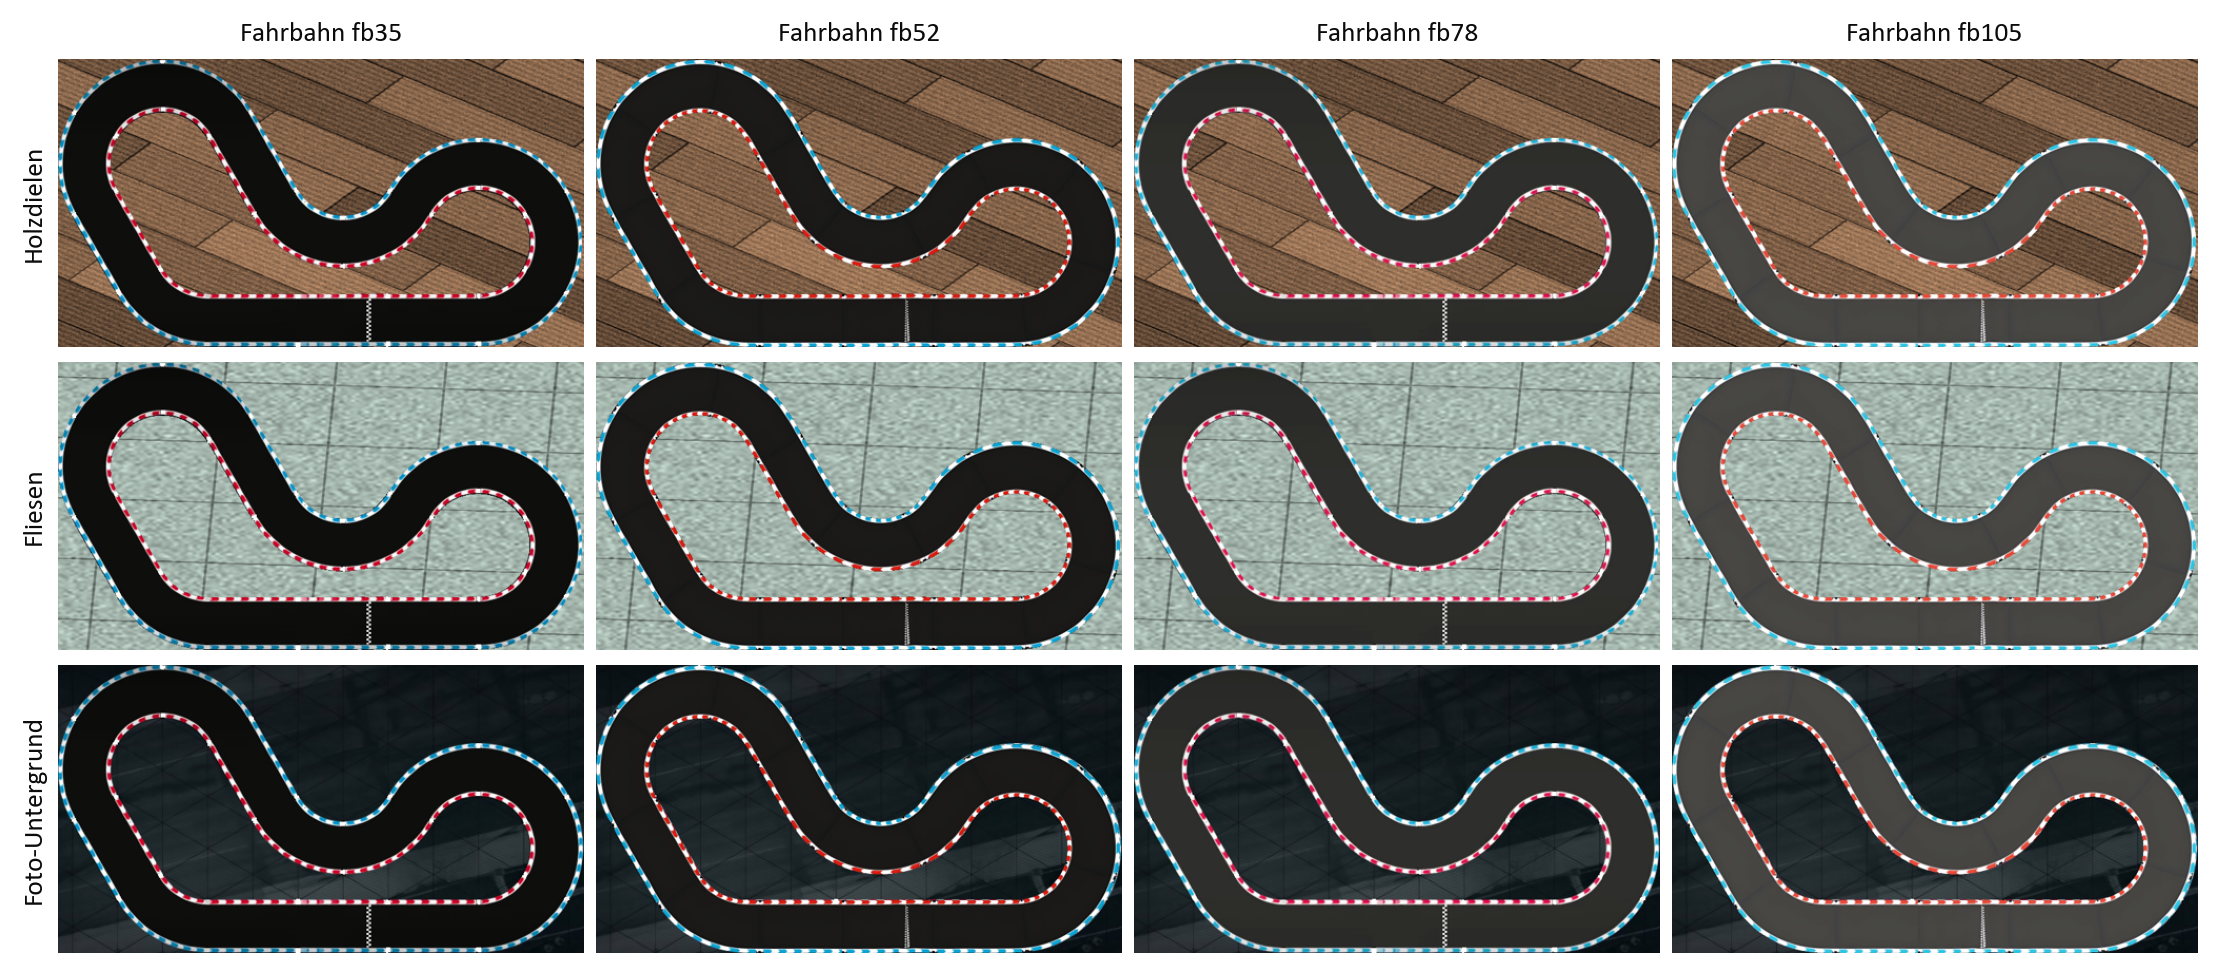
\includegraphics[width=\linewidth]{chapters/felix_teil/bilder/darstellungen.png}
  \caption{Die zwölf Darstellungen der Trainingsstrecke: drei Untergründe (Zeilen) und vier Helligkeiten der Fahrbahn (Spalten).}
  \label{fig:darstellungen}
\end{figure}

Weiterhin wird das Bild für Agent~2 auf vier Graustufen reduziert. Feine Unterschiede der Oberflächen verschwinden dadurch weitgehend, während Fahrbahn, Randsteine und Fahrzeug unterscheidbar bleiben. Zugleich lassen sich die Bilder mit \SI{2}{\bit} je Pixel im Erfahrungsspeicher ablegen.

\subsubsection{Das Training}
\label{subsec:agent2_training}

Agent~2 wird mit 16 parallelen Umgebungen trainiert. Der vortrainierte Encoder wird vollständig übernommen und bleibt bis 2~Mio.\ Übergänge eingefroren. Seine erste vollständige Runde fährt der Agent nach \num{3.9}~Mio.\ Übergängen. Das fertige Modell wurde über \num{14.5}~Mio.\ Übergänge in rund \SI{92}{\hour} trainiert.

Abbildung~\ref{fig:agent2_verlauf} zeigt den Trainingsverlauf. Die Kurven enthalten das Explorationsrauschen und sind über alle Darstellungen gemittelt. Sie liegen daher deutlich unter den deterministisch gemessenen Werten. Zwischen \num{4.4} und 5~Mio.\ Übergängen stieg der Verlust des Critics um das Hundertfache, und das Fahren brach vorübergehend ein. Zeitlich fällt das mit den ersten Runden zusammen, deren Bonus die Zielwerte des Critics sprunghaft erhöht. Der Encoder blieb dabei intakt, und der Agent erholte sich ohne Eingriff. Das ist ein Hinweis zu der in Phase~1 offenen Frage, warum \ac{SAC}-Läufe nach ihrem Höhepunkt einbrechen (Abschnitt~\ref{subsec:ppo_sac_vergleich}), aber keine Erklärung.

\begin{figure}[htbp]
  \centering
  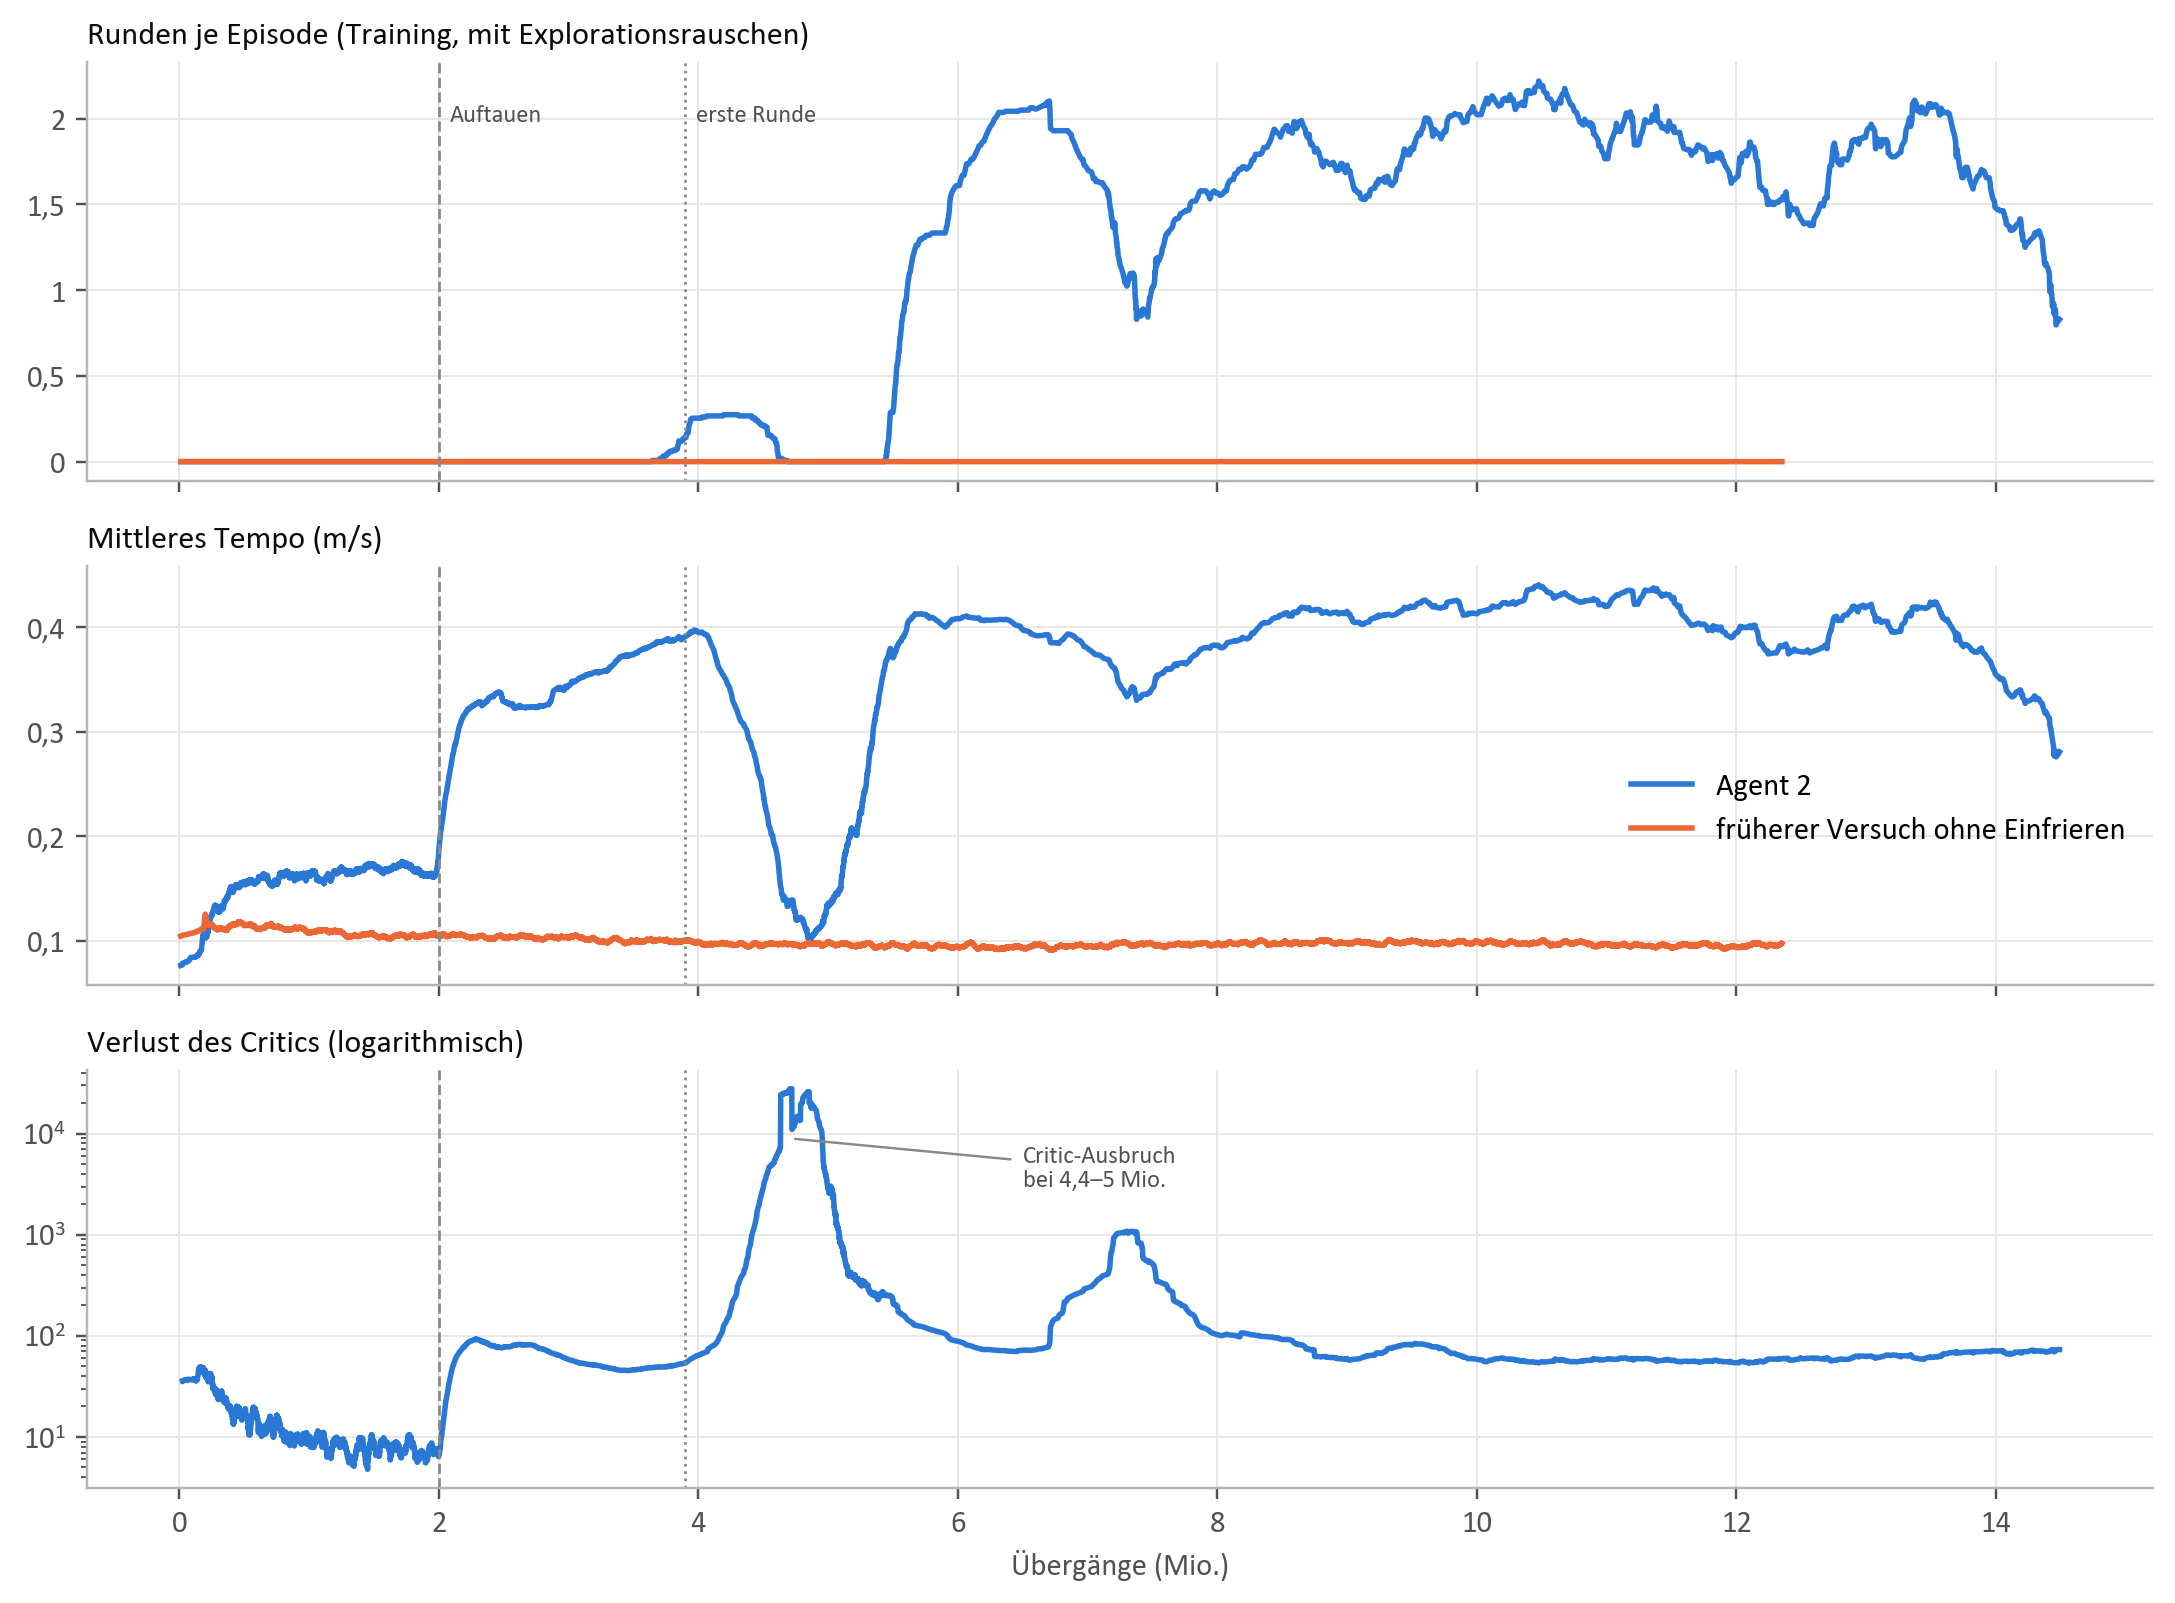
\includegraphics[width=\linewidth]{chapters/felix_teil/bilder/agent2_verlauf.png}
  \caption{Trainingsverlauf von Agent~2 im Vergleich zu einem früheren Versuch ohne Einfrieren (Werte mit Explorationsrauschen). Gestrichelt: Auftauen; gepunktet: erste vollständige Runde.}
  \label{fig:agent2_verlauf}
\end{figure}

\subsubsection{Das Ergebnis}
\label{subsec:agent2_ergebnis}

Abbildung~\ref{fig:agent2_darstellungen} zeigt das Ergebnis von Agent~2 nach \num{14.5}~Mio.\ Übergängen auf allen zwölf Darstellungen. Im Mittel fährt er \num{4.5} Runden je Episode bei einem Tempo von \SI{0.53}{\meter\per\second}. Die beste Runde dauert \SI{9.65}{\second}, und \SI{31}{\percent} der Episoden enden mit einem Crash. Auf allen zwölf Darstellungen fährt er Runden, auf sieben davon im Mittel mindestens fünf.

\begin{figure}[htbp]
  \centering
  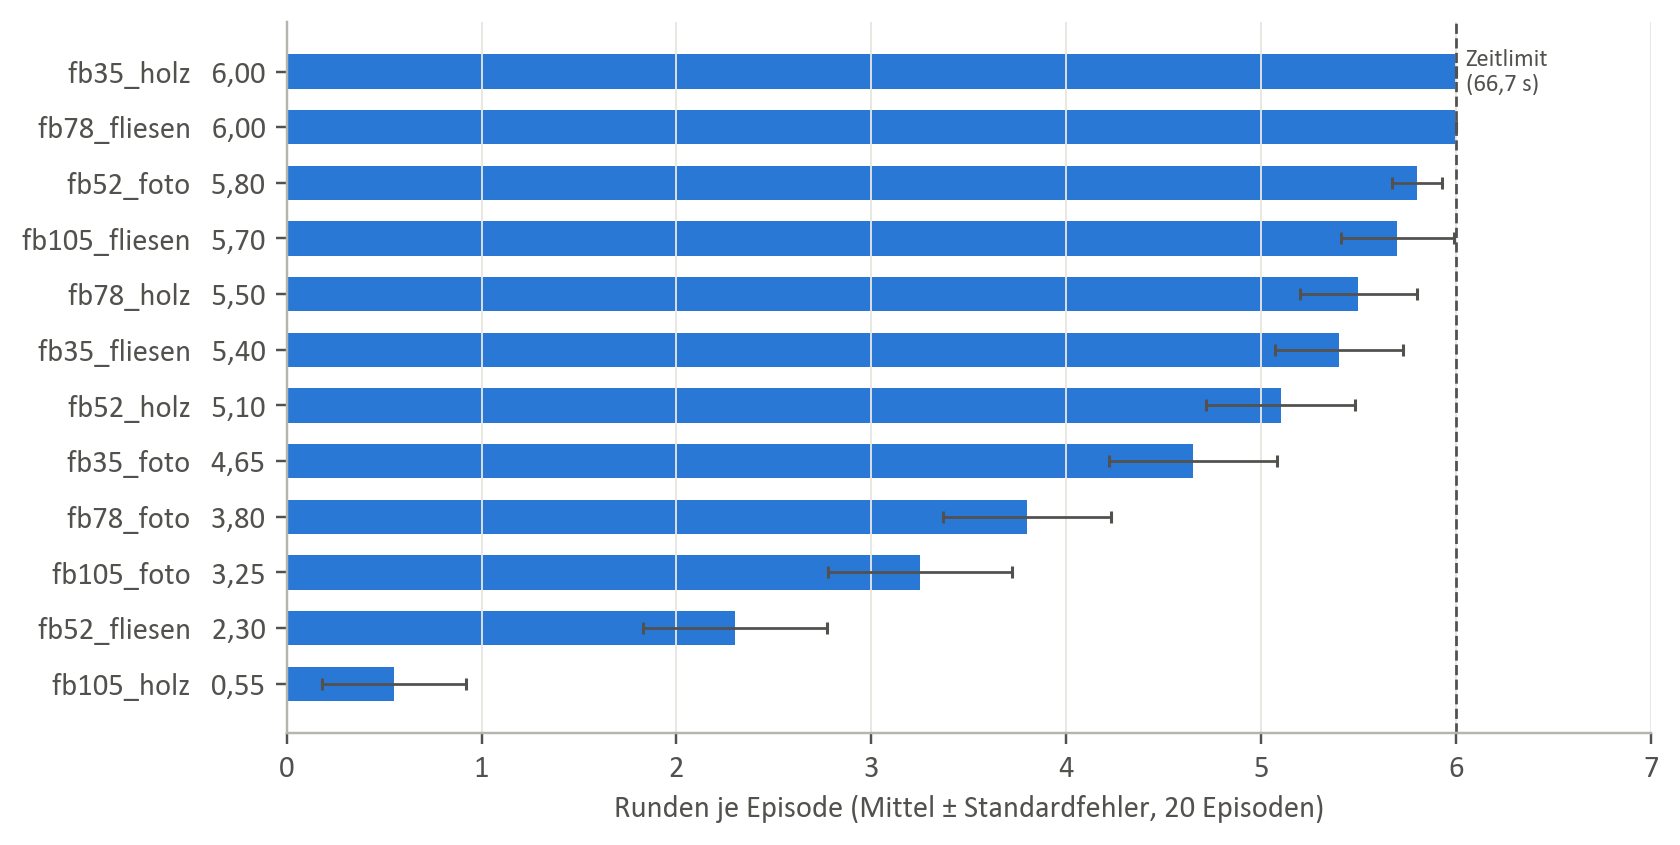
\includegraphics[width=0.9\linewidth]{chapters/felix_teil/bilder/agent2_darstellungen.png}
  \caption{Agent~2 auf den zwölf Darstellungen (je 20 Episoden à \SI{66.67}{\second}, deterministisch). Bei 6 Runden liegt das Zeitlimit. Die Werte der unteren Darstellungen sind Grenzfälle und schwanken zwischen Messungen; für \texttt{fb105\_holz} lagen sie in verschiedenen Messungen zwischen 0 und 4 Runden.}
  \label{fig:agent2_darstellungen}
\end{figure}

Drei Darstellungen erreichen bei \SI{66.67}{\second} das Zeitlimit von sechs Runden in jeder Episode, die Messung zeigt dort also nicht das Können, sondern die Episodenlänge. Mit \SI{200}{\second} langen Episoden fährt Agent~2 auf diesen drei Darstellungen \num{19} bis \num{19.7} Runden ohne einen einzigen Crash, im Mittel über alle zwölf \num{12.4} Runden.

\paragraph{Gegenprobe mit Agent~1.}
Als Gegenprobe wurde Agent~1 auf denselben zwölf Darstellungen gemessen: Er fährt auf keiner einzigen eine Runde und verlässt nach etwa einer Sekunde die Fahrbahn. Die Verallgemeinerung von Agent~2 ist damit nicht nur behauptet, sondern gegen ein Modell ohne Randomisierung geprüft.

\paragraph{Wo die schwachen Darstellungen scheitern.}
Auf den Darstellungen mit vielen Crashes verlässt der Agent fast immer in derselben Kurve die Fahrbahn. Der Hergang ist jedes Mal gleich: Innerhalb von \SI{0.3}{\second} wächst der Richtungsfehler von nahezu null auf über \SI{30}{\degree}, und der Gegenlenkbefehl kommt zu spät. Das Tempo ist dabei nicht die Ursache; auf einer sicher gefahrenen Darstellung durchfährt er dieselbe Kurve sogar schneller. Auch die Sichtbarkeit ist es nicht: Der Encoder liest die Lage auf der schwächsten Darstellung genauer ab als auf mancher sicher gefahrenen. Der Agent hat an dieser Stelle schlicht eine sehr kleine Reserve, sodass jede kleine Änderung der Eingabe das Ergebnis umkippen kann.

\paragraph{Feinere Graustufen.}
Dazu passt ein überraschender Befund. Wird das Kamerabild bei der Messung auf acht statt auf die trainierten vier Graustufen reduziert, sinkt die Crashrate auf der Darstellung \texttt{fb52\_fliesen} von \SI{80}{\percent} auf \SI{0}{\percent}, ohne jedes Nachtraining, auch mit 16 und 256 Stufen gab es keinen Crash. Der Agent verträgt also feinere Eingaben als die, auf denen er trainiert wurde. Für die Übertragung auf eine echte Kamera mit 256 Graustufen ist das die günstige Richtung.

\paragraph{Lohnt sich das lange Training?}
Agent~2 wurde nach \num{6.5} und nach \num{14.5}~Mio.\ Übergängen gemessen. Die Differenz von \num{0.54} Runden je Episode liegt innerhalb der Messunsicherheit (Standardfehler \num{0.61}), und die spätere Fassung ist nur auf sieben von zwölf Darstellungen besser. Sicher nachweisbar ist nur, dass sie schneller fährt, auf allen zwölf Darstellungen, mit kürzeren Rundenzeiten. Die zweite Hälfte des Trainings, rund \SI{50}{\hour}, hat also im Wesentlichen das Tempo verbessert, nicht die Zuverlässigkeit.

\subsection{Vergleich der beiden Modelle}
\label{sec:agentenvergleich}

Tabelle~\ref{tab:agentenvergleich} stellt Agent~1 und Agent~2 gegenüber. Die beiden Modelle lösen verschiedene Aufgaben und sind deshalb nicht direkt vergleichbar. Agent~1 fährt auf einer Darstellung und ist auf diese spezialisiert. Agent~2 dagegen fährt auf 12 unterschiedlichen Darstellungen.

\begin{table}[htbp]
  \centering
  \caption{Die beiden fahrenden Kamera-Agenten.}
  \label{tab:agentenvergleich}
  \small
  \begin{tabularx}{\linewidth}{@{}l X X@{}}
    \toprule
     & \textbf{Agent~1} & \textbf{Agent~2} \\
    \midrule
    Aufgabe                          & 1 Darstellung & 12 Darstellungen mit Bildstörungen \\
    Vortraining                      & \ac{BC} eines Lehrers (Fahrwissen) & Encoder für Versatz und Richtung (nur Sehwissen) \\
    Eingefroren                      & Faltungen bis \num{0.3}~Mio.\ Übergänge & gesamter Encoder bis 2~Mio.\ Übergänge \\
    Parallele Umgebungen             & 4 & 16 \\
    Graustufen                       & 256 & 4 \\
    Speicher je Umgebung             & \SI{69}{\minute} Fahrt & \SI{104}{\minute} Fahrt \\
    Übergänge bis zur ersten Runde   & \num{0.92}~Mio. & \num{3.9}~Mio. \\
    Übergänge im fertigen Modell     & \num{2.2}~Mio. & \num{14.5}~Mio. \\
    Runden je Episode (\SI{66.67}{\second}) & \num{6.4} auf seiner Darstellung, 0 auf den 12 anderen & \num{4.5} im Mittel über 12 \\
    Beste Runde                      & \SI{8.65}{\second} & \SI{9.65}{\second} \\
    Episoden mit Crash               & \SI{10}{\percent} & \SI{31}{\percent} \\
    \bottomrule
  \end{tabularx}
\end{table}

Neben der Aufgabe unterscheiden sich die beiden Agenten vor allem im Vortraining. Agent~1 hat Fahrwissen vom Lehrer geerbt, Agent~2 hat nur gelernt, wo das Auto auf der Bahn liegt, und das Fahren vollständig selbst gelernt. Dass Agent~2 viermal so viele Übergänge bis zur ersten Runde braucht, ist vor diesem Hintergrund und bei zwölffacher Aufgabe nicht überraschend.

\subsection{Test des zweiten Agenten auf anderen Streckenführungen}
\label{sec:andere_strecken}

Agent~2 fährt auf allen zwölf Darstellungen der Trainingsstrecke. Offen ist, ob er damit das Fahren an sich gelernt hat oder nur diese eine Streckenführung. Dazu wird er zunächst ohne weiteres Training auf neuen Streckenführungen getestet und anschließend auf zwei davon weitertrainiert.

\subsubsection{Test ohne Nachtraining}
\label{subsec:ohne_nachtraining}

Agent~2 wird ohne weiteres Training auf vier neuen Streckenführungen (\texttt{kurs\_A} bis \texttt{kurs\_D}) getestet, die mit dem Streckengenerator aus Abschnitt~\ref{subsec:agent2_darstellung} erzeugt wurden. Damit sich nur die Führung verändert und nicht gleichzeitig das Aussehen, wurden für \texttt{kurs\_A} dieselben zwölf Darstellungen erzeugt, auf denen Agent~2 trainiert wurde (Tabelle~\ref{tab:ohne_nachtraining}).

\begin{table}[htbp]
  \centering
  \caption{Agent~2 ohne Nachtraining (deterministisch).}
  \label{tab:ohne_nachtraining}
  \small
  \begin{tabular}{@{}l l l@{}}
    \toprule
    \textbf{Strecke} & \textbf{Darstellung} & \textbf{Runden je Episode} \\
    \midrule
    Original                              & trainiert (12) & \num{4.5} (\SI{66.67}{\second}) bzw.\ \num{12.4} (\SI{200}{\second}) \\
    Original                              & unbekannt      & \num{2.3} \\
    \texttt{kurs\_A}                      & trainiert (12) & \num{0.00} auf allen 12 \\
    \texttt{kurs\_A} bis \texttt{kurs\_D} & unbekannt      & \num{0.00} \\
    \bottomrule
  \end{tabular}
\end{table}

Eine unbekannte Darstellung der bekannten Strecke fährt der Agent noch mit \num{2.3} Runden. Eine unbekannte Streckenführung fährt er dagegen nicht, auch wenn sie in den bekannten Darstellungen gezeigt wird. Sein Verhalten auf \texttt{kurs\_A} ist dabei kein schlechteres Fahren, sondern eine Sättigung, voller Lenkeinschlag, Vollgas und Vollbremse gleichzeitig, ohne jede Korrektur. Es ist dasselbe Muster wie bei den blinden Agenten, obwohl der Encoder hier intakt ist.

Besonders aufschlussreich ist, dass \texttt{kurs\_A} die um \SI{180}{\degree} gedrehte Originalstrecke ist. Der Agent hat also nicht die Form der Strecke gelernt, sondern die Form in dieser Lage im Kamerabild. Für eine fest montierte Kamera über einer festen Strecke ist das kein Nachteil. Ein Agent, der jede beliebige Strecke fährt, entsteht so aber nicht.

\subsubsection{Weitertrainieren von Agent~2 gegen Neustart}
\label{subsec:weitertrainieren}

Da Agent~2 neue Streckenführungen ohne weiteres Training nicht fährt, wird untersucht, ob sein Vorwissen das Erlernen einer neuen Strecke zumindest beschleunigt. Dazu wird auf zwei Streckenführungen jeweils ein Weitertraining von Agent~2 mit einem Neustart verglichen:

\begin{description}
  \item[Weitertraining:] ausgehend vom fertigen Agent~2, also mit seinem Encoder und seiner Fahrweise;
  \item[Neustart:] ein neuer Agent mit demselben vortrainierten Encoder wie zu Beginn von Agent~2, eingefroren bis 2~Mio.\ Übergänge.
\end{description}

Als Strecken dienen \texttt{kurs\_A}, die gedrehte Originalstrecke, und \texttt{kurs\_D}, deren Fahrbahnfläche sich im Kamerabild nur zu \SI{21}{\percent} mit der Originalstrecke deckt. Gemessen wurde, nach wie vielen Übergängen die erste vollständige Runde fällt (Tabelle~\ref{tab:transfer}, Abbildung~\ref{fig:transfer}).

\begin{table}[htbp]
  \centering
  \caption{Übergänge bis zur ersten vollständigen Runde.}
  \label{tab:transfer}
  \small
  \begin{tabularx}{\linewidth}{@{}X l l l@{}}
    \toprule
    \textbf{Strecke} & \textbf{Weitertraining} & \textbf{Neustart} & \textbf{Ersparnis} \\
     & \textbf{(von Agent~2)} & \textbf{(nur Encoder)} & \\
    \midrule
    \texttt{kurs\_A} (Original, um \SI{180}{\degree} gedreht) & \num{2.81}~Mio. & \num{2.90}~Mio. & \SI{3}{\percent} \\
    \texttt{kurs\_D} (unähnlichste Führung)                   & \num{2.92}~Mio. & \num{3.29}~Mio. & \SI{11}{\percent} \\
    zum Vergleich: Agent~2 auf der Originalstrecke            & --              & \num{3.90}~Mio. & -- \\
    \bottomrule
  \end{tabularx}
\end{table}

\begin{figure}[htbp]
  \centering
  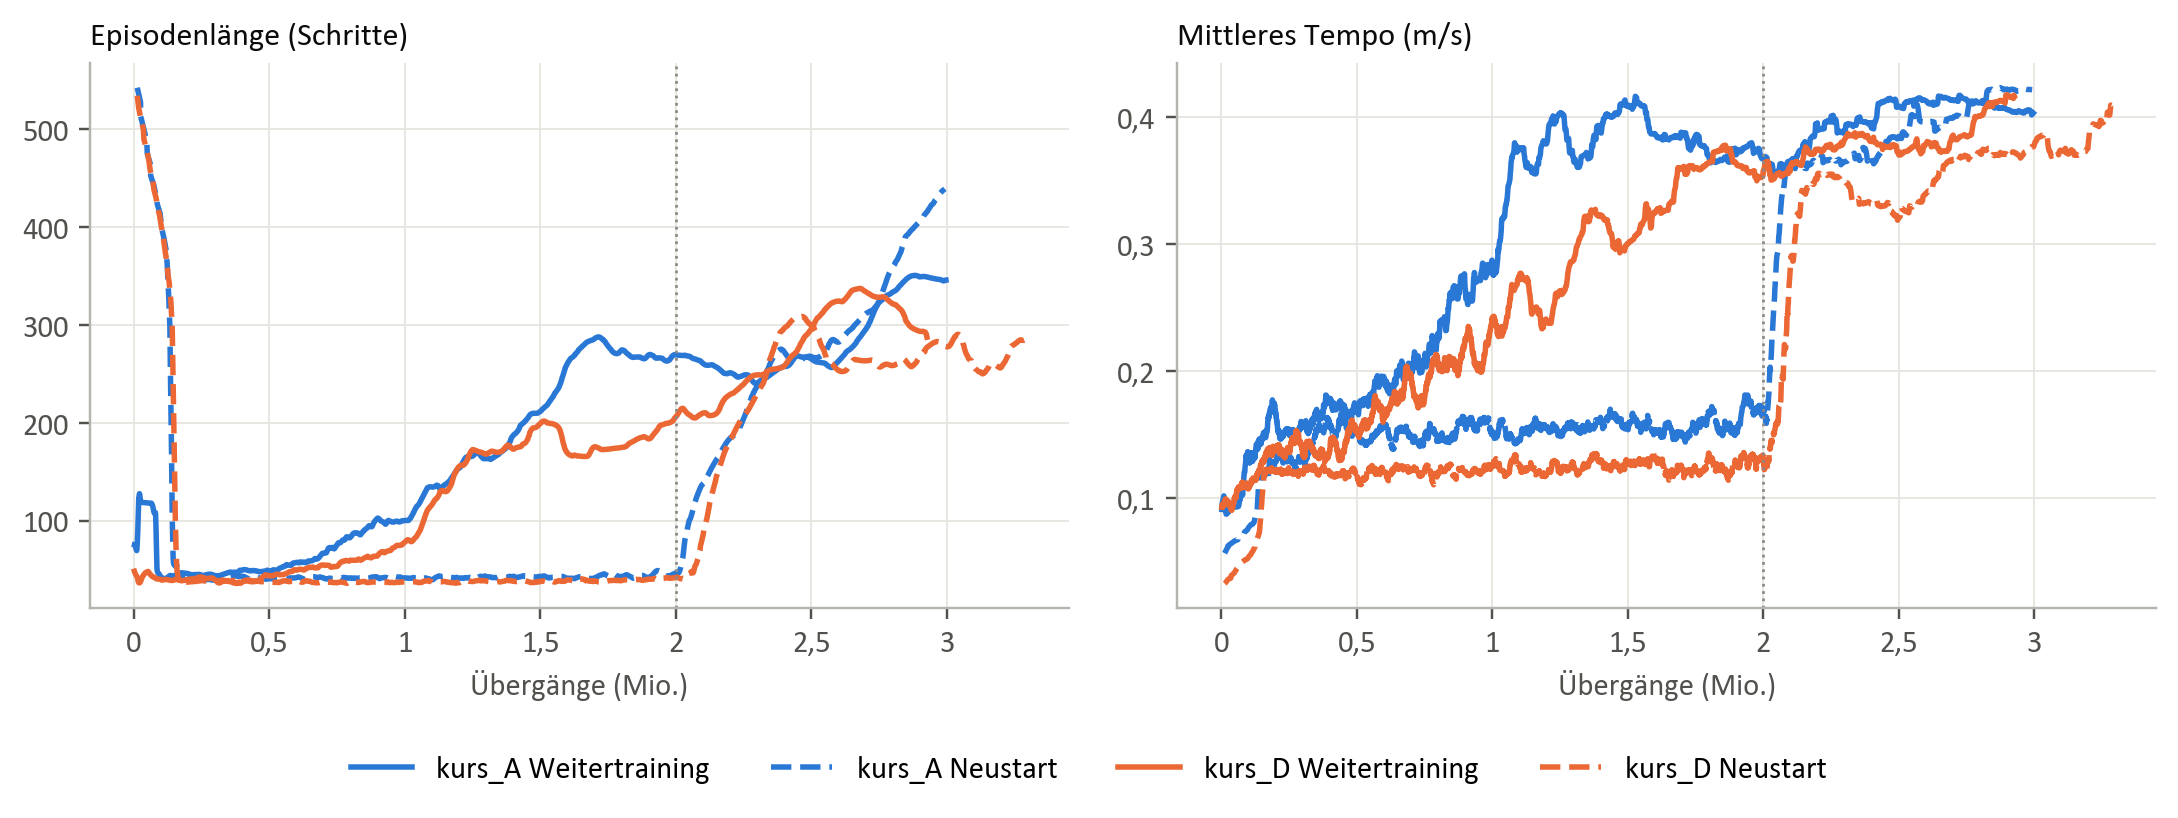
\includegraphics[width=\linewidth]{chapters/felix_teil/bilder/transfer.png}
  \caption{Weitertrainieren (durchgezogen) gegen Neustart (gestrichelt) auf \texttt{kurs\_A} (blau) und \texttt{kurs\_D} (orange). Bei 2~Mio.\ Übergängen wird der Encoder der Neustarts aufgetaut.}
  \label{fig:transfer}
\end{figure}

Das Vorwissen aus dem Training von Agent~2 bringt wenig: \SI{3}{\percent} auf \texttt{kurs\_A} und \SI{11}{\percent} auf \texttt{kurs\_D}. Da je Bedingung nur ein Lauf gefahren wird, kann ein Unterschied von \SI{3}{\percent} auch zufällig entstehen. Abbildung~\ref{fig:transfer} zeigt, woher der Unterschied kommt. Der weitertrainierte Agent lernt von Beginn an, weil sein Encoder nicht eingefroren werden muss, und ist nach \num{600000} bis \num{800000} Übergängen deutlich weiter. Sobald der Encoder des neu gestarteten Agenten bei 2~Mio.\ Übergängen aufgetaut wird, holt dieser den Rückstand innerhalb von etwa \num{600000} Übergängen auf.

Übertragbar ist damit das \emph{Sehen}, also die Fähigkeit, die Lage des Fahrzeugs im Bild abzulesen. Die \emph{Fahrweise} ist nicht übertragbar. Der Agent lernt nicht das allgemeine Fahren, sondern diese eine Strecke in dieser einen Kameraansicht.

Zwei Einschränkungen gelten für diesen Vergleich. Zum einen wird der Encoder des neu gestarteten Agenten auf Bildern der Originalstrecke trainiert. Beide Bedingungen bringen also Vorwissen von der Originalstrecke mit, und gemessen wurde genau der Beitrag der Fahrweise. Wie viel der Encoder auf einer fremden Strecke beiträgt, wurde nicht gemessen. Ein Neustart ganz ohne Encoder wurde dort nicht gefahren. Zum anderen musste der Neustart auf \texttt{kurs\_D} ab 3~Mio.\ Übergängen mit leerem Erfahrungsspeicher fortgesetzt werden, weil sich der gesicherte Speicher nicht laden ließ. Das hat ihn vermutlich gebremst; die \SI{11}{\percent} sind daher eher eine Obergrenze.

     % Felix: Phase 2, Umsetzung in 3D
% 06-trainingsablauf.tex
\section{Trainingsablauf in Isaac}
\label{sec:trainingsablauf}

Wie in Phase~1 gezeigt, ist es von Vorteil, das \ac{RL}-Training nicht ohne Vorbereitung zu starten. Ein Kamera-Agent, der von Null an lernt, muss zwei Dinge gleichzeitig herausfinden: was die Pixel bedeuten und wie man fährt. Das einzige Signal dafür ist die Belohnung. Um das zu erleichtern, wird der Bildteil des Netzes vorab überwacht trainiert. Anschließend folgen die beiden fahrenden Kamera-Agenten, die im Verlauf der Arbeit entstanden sind, im Folgenden Agent~1 und Agent~2. Beide durchlaufen dieselben vier Stufen, unterscheiden sich aber im Ziel des Vortrainings und in den Darstellungen der Strecke: Agent~1 lernt auf einer einzigen Darstellung, Agent~2 auf zwölf.

\subsection{Die Trainingspipeline in 3D}
\label{sec:pipeline3d}

Entsprechend der Python-Umgebung wird auch hier eine mehrstufige Trainingspipeline verwendet, um den Ablauf des \ac{RL}-Trainings effizienter zu gestalten. Diese Pipeline besteht aus vier separaten Stufen, wie in Abbildung~\ref{fig:pipeline_stufen} zu sehen.

\begin{figure}[htbp]
  \centering
  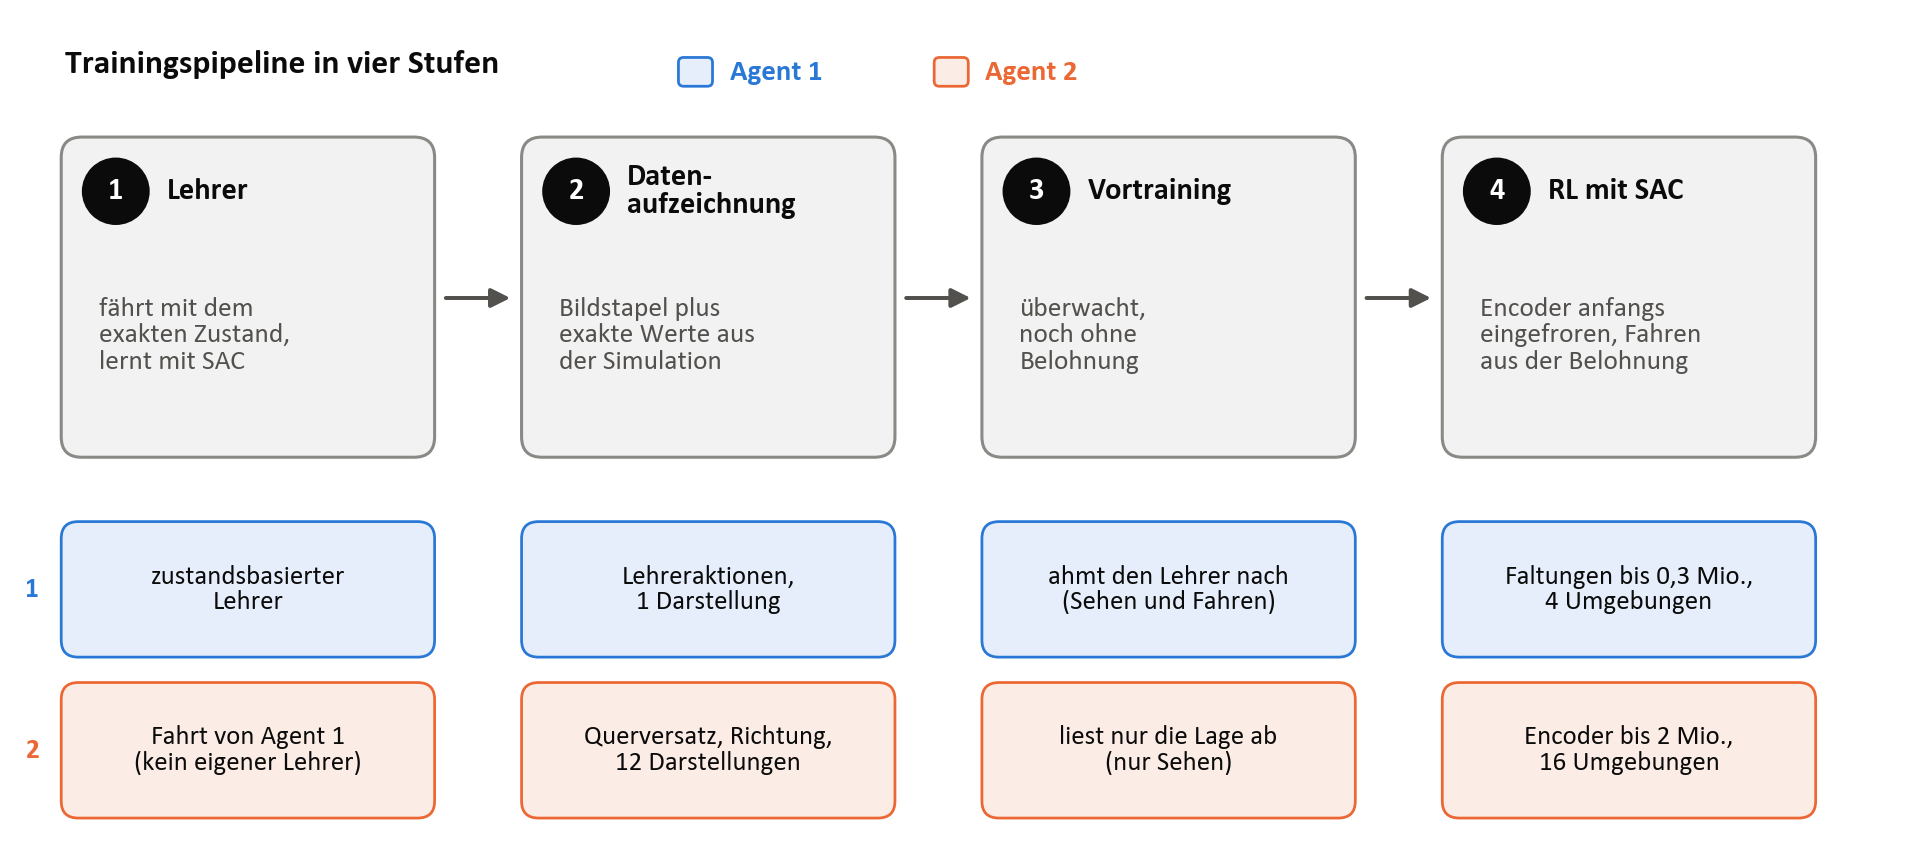
\includegraphics[width=\linewidth]{chapters/felix_teil/bilder/pipeline_stufen.png}
  \caption{Trainingspipeline in vier Stufen. Oben der gemeinsame Ablauf, darunter die Unterschiede zwischen Agent~1 (blau) und Agent~2 (orange).}
  \label{fig:pipeline_stufen}
\end{figure}

\paragraph{Stufe 1 -- Lehrer.}
Wie in Phase~1 wird zuerst ein Agent trainiert, der als Lehrer für den späteren bildbasierten Agenten dient (Abschnitt~\ref{subsec:privileged}). Während der Lehrer in der 2D-Umgebung anhand von Lidar-Strahlen lernte, ist er hier zustandsbasiert. Er erhält den exakten Zustand aus der Simulation, also Geschwindigkeit, Drehrate, Richtungsfehler, Querversatz und die Abstände zu beiden Fahrbahnkanten, sowie seine letzte Aktion. Da Isaac alle diese Größen ohnehin kennt, ist es nicht nötig, Abstandsstrahlen nachzubilden.

Dieser Lehrer wird mit \ac{SAC} auf 64 parallelen Umgebungen trainiert und fährt nach \num{768000} Übergängen 8 Runden je Episode ohne Crash, mit einer Rundenzeit von ca.\ \SI{8.3}{\second}. Damit ist gezeigt, dass Physik und Belohnungsfunktion in 3D lösbar sind.

\paragraph{Stufe 2 -- Datenaufzeichnung.}
Anschließend fährt der Lehrer in der Kamera-Umgebung. Zu jedem Schritt werden der Bildstapel und die Aktion des Lehrers gespeichert, insgesamt \num{48000} Paare. Abweichend von Phase~1 fährt der Lehrer dabei deterministisch, ohne injiziertes Rauschen (Gleichung~\eqref{eq:noise}), Vielfalt im Datensatz entsteht nur durch die zufälligen Startpositionen. Für Agent~2 stammen die Bilder stattdessen aus einer Fahrt von Agent~1, die in allen zwölf Darstellungen der Strecke gerendert wird (Abschnitt~\ref{sec:agent2}).

\paragraph{Stufe 3 -- Vortraining.}
Vortrainiert wird der Teil des Netzes, der aus dem Bildstapel Merkmale berechnet, im Folgenden Merkmalsextraktor (Encoder). Er besteht wie in Phase~1 aus den drei Faltungsschichten des NatureCNN \cite{mnih2015human} und einer voll verbundenen Schicht mit 512 Neuronen. Für Agent~1 lernt das Netz analog zu Phase~1, die Aktionen des Lehrers nachzuahmen (\ac{BC}, Abschnitt~\ref{subsec:il}). Bestätigt wurde dabei die Warnung aus Abschnitt~\ref{sec:ergebnisse_pipeline}, dass ein niedriger Vorhersagefehler kein Fahrkönnen belegt: Von zwei Netzen fuhr das mit dem schlechteren Fehler ($R^2 = \num{0.25}$ gegen \num{0.47}) \SI{60}{\percent} weiter. Nach dem Vorhersagefehler wäre das schlechtere Netz ausgewählt worden. Vortrainierte Netze wurden deshalb im Fahrversuch bewertet, nicht am Verlust.

Für Agent~2 lernt der Encoder dagegen nicht die Aktionen, sondern nur die Lage des Fahrzeugs, Querversatz zur Mittellinie und Richtungsfehler, beide aus der Simulation exakt bekannt. Vortrainiert wird damit nur das Sehen, nicht das Fahren, wie auf eine Situation zu reagieren ist, lernt der Agent erst im \ac{RL}-Training.

\paragraph{Stufe 4 -- Online-Training mit SAC.}
Die vortrainierten Gewichte werden in das Netz des \ac{RL}-Agenten übertragen und als Grundlage für das \ac{SAC}-Training verwendet. Für Agent~1 werden nur die Faltungsschichten übernommen, für Agent~2 der gesamte Encoder. Der Kopf hinter dem Encoder, der aus den Merkmalen die Aktionen und ihre Bewertung berechnet, ist zu Beginn zufällig initialisiert.

Gerade am Anfang des Trainings sind die Gradienten des Reinforcement Learning stark verrauscht, der Agent verlässt nach wenigen Schritten die Fahrbahn, und der Critic kann den Wert einer Aktion kaum einschätzen. Lernt der Encoder in dieser Phase mit, überschreiben diese Gradienten das vortrainierte Sehen, bevor der Kopf gelernt hat, es zu nutzen.

Der Encoder wird deshalb zu Beginn eingefroren: Seine Gewichte bleiben für eine festgelegte Zahl von Übergängen unverändert, und nur der Kopf lernt. Danach wird der Encoder aufgetaut und lernt mit. Die Gradienten verfeinern das Sehen nun, statt es zu zerstören. Bei Agent~1 waren die Faltungsschichten bis \num{0.3}~Mio.\ Übergänge eingefroren, bei Agent~2 der gesamte Encoder bis 2~Mio. Wie entscheidend dieser Schritt ist, zeigt ein Gegenversuch (Abschnitt~\ref{sec:einfrieren}).

\subsection{Training des Kamera-Agenten}
\label{sec:kamera_training}

Der Kamera-Agent wird, wie in Phase~1 erarbeitet, mit \ac{SAC} trainiert (Abschnitte~\ref{subsec:ppo_sac} und~\ref{subsec:ppo_sac_vergleich}); auch die Netzarchitektur, das NatureCNN, stammt aus Phase~1. Actor und Critic besitzen jeweils einen eigenen Encoder, dahinter je einen Kopf, der die drei Aktionen bzw.\ deren Bewertung berechnet.

Während des Trainings fährt der Agent parallel in mehreren Umgebungen. Jeder Übergang landet im Erfahrungsspeicher, aus dem nach jedem Simulationsschritt Stichproben für die Updates gezogen werden. Die Aktionen sind dabei zufällig gestreut, damit der Agent erkundet.

Als Eingabe erhält der Agent ausschließlich den Bildstapel. Belohnung, frühere Aktionen oder die Geschwindigkeit werden nicht zurückgeführt, die Belohnung dient nur als Lernsignal für den Critic.

\paragraph{Bewertung.}
Die Agenten werden nach dem Training deterministisch bewertet, also ohne Zufallsanteil der Aktionen und ohne Bildstörungen, mit zufälligen Startpositionen und getrennt je Darstellung der Strecke. Dabei werden Runden je Episode, mittleres Tempo, beste Rundenzeit und der Anteil der Episoden, die mit einem Crash enden, gemessen. Die Werte aus dem Training eignen sich dafür nicht, weil die Aktionen dort zufällig gestreut und über alle Darstellungen gemittelt sind. Da gute Agenten in \SI{66.67}{\second} das Zeitlimit von etwa sechs Runden erreichen, wurden die fertigen Modelle zusätzlich mit \SI{200}{\second} langen Episoden gemessen.

\subsection{Probleme auf dem Weg zum ersten Agenten}
\label{sec:probleme_agent1}

Bis zum ersten fahrenden Kamera-Agenten vergingen etwa \SI{125}{\hour} Rechenzeit in Läufen, die nichts lernen konnten. Die wesentlichen Fehler traten ohne Absturz oder Warnung auf. Mehrere Fehler betrafen die Vortrainingskette: invertierte Lehrerbilder, Lehreraktionen außerhalb des gültigen Wertebereichs und das Speichern der letzten statt der besten Trainingsepoche.

Auch mit korrektem Bild lernte der Agent zunächst nicht zu fahren. Zum einen bestand eine Belohnungsfalle: Ohne den Fortschrittsterm brachte Geradeausfahren erst ab \SI{0.52}{\meter\per\second} Pluspunkte, sodass ein schnelles Verlassen der Fahrbahn für den Agenten günstiger war als langsames Weiterfahren. Erst der Fortschrittsterm (Abschnitt~\ref{subsec:3d_belohnung}) beseitigte diese Falle. Zum anderen verlor der Agent seine vortrainierte Sehfähigkeit. Das vortrainierte Netz fuhr allein 120 Schritte weit, der Agent nach \num{762000} Übergängen nur noch 44 und damit kürzer als ein Fahrzeug, das ohne Lenken 86 Schritte weit fährt. Das \ac{RL} hatte die vortrainierten Merkmale überschrieben.

\subsection{Einfrieren des Encoders}
\label{sec:einfrieren}

Wie wichtig das Einfrieren des Encoders ist, zeigt ein Gegenversuch: zwei Läufe mit identischem Aufbau, einmal mit eingefrorenem Encoder bis 2~Mio.\ Übergänge und einmal ohne Einfrieren. Der Aufbau entspricht dem von Agent~2 (Abschnitt~\ref{sec:agent2}).

Neben der Episodenlänge werden dafür zwei Kennzahlen aufgezeichnet, beide auf einer Stichprobe von Bildern aus dem Erfahrungsspeicher. Die erste ist der Anteil inaktiver Neuronen der 512er-Schicht, also der Neuronen, die für alle Bilder der Stichprobe null ausgeben. Ein solches Neuron trägt keine Information über das Bild mehr, ist fast die gesamte Schicht inaktiv, erreicht den Kopf des Netzes kaum noch Bildinformation. Die zweite ist die Streuung des Lenkbefehls über die Bilder der Stichprobe. Ist sie null, gibt der Agent für jedes Bild denselben Lenkbefehl aus, er ist blind. In den üblichen Trainingskurven ist beides nicht zu erkennen, sie verlaufen lediglich flach. Tabelle~\ref{tab:gegenversuch_einfrieren} und Abbildung~\ref{fig:gegenversuch_einfrieren} zeigen den Verlauf.

\begin{table}[htbp]
  \centering
  \caption{Gegenversuch Einfrieren, Werte im Trainingsverlauf (Episodenlänge in Schritten / Anteil inaktiver Neuronen der 512er-Schicht / Streuung des Lenkbefehls).}
  \label{tab:gegenversuch_einfrieren}
  \small
  \begin{tabular}{@{}l c c@{}}
    \toprule
    \textbf{Übergänge} & \textbf{ohne Einfrieren} & \textbf{eingefroren bis 2~Mio.} \\
    \midrule
    \num{0.5}~Mio.  & 33 / \SI{89}{\percent} / \num{0.000}   & 42 / \SI{81}{\percent} / \num{0.99} \\
    \num{2.0}~Mio.  & 31 / \SI{92}{\percent} / \num{0.000}   & 58 / \SI{63}{\percent} / \num{0.91} \\
    \num{2.5}~Mio.  & 31 / \SI{96}{\percent} / \num{0.000}   & 270 / \SI{22}{\percent} / \num{1.49} \\
    \num{2.95}~Mio. & 31 / \SI{99.6}{\percent} / \num{0.000} & 444 / \SI{18}{\percent} / \num{1.42} \\
    \bottomrule
  \end{tabular}
\end{table}

\begin{figure}[htbp]
  \centering
  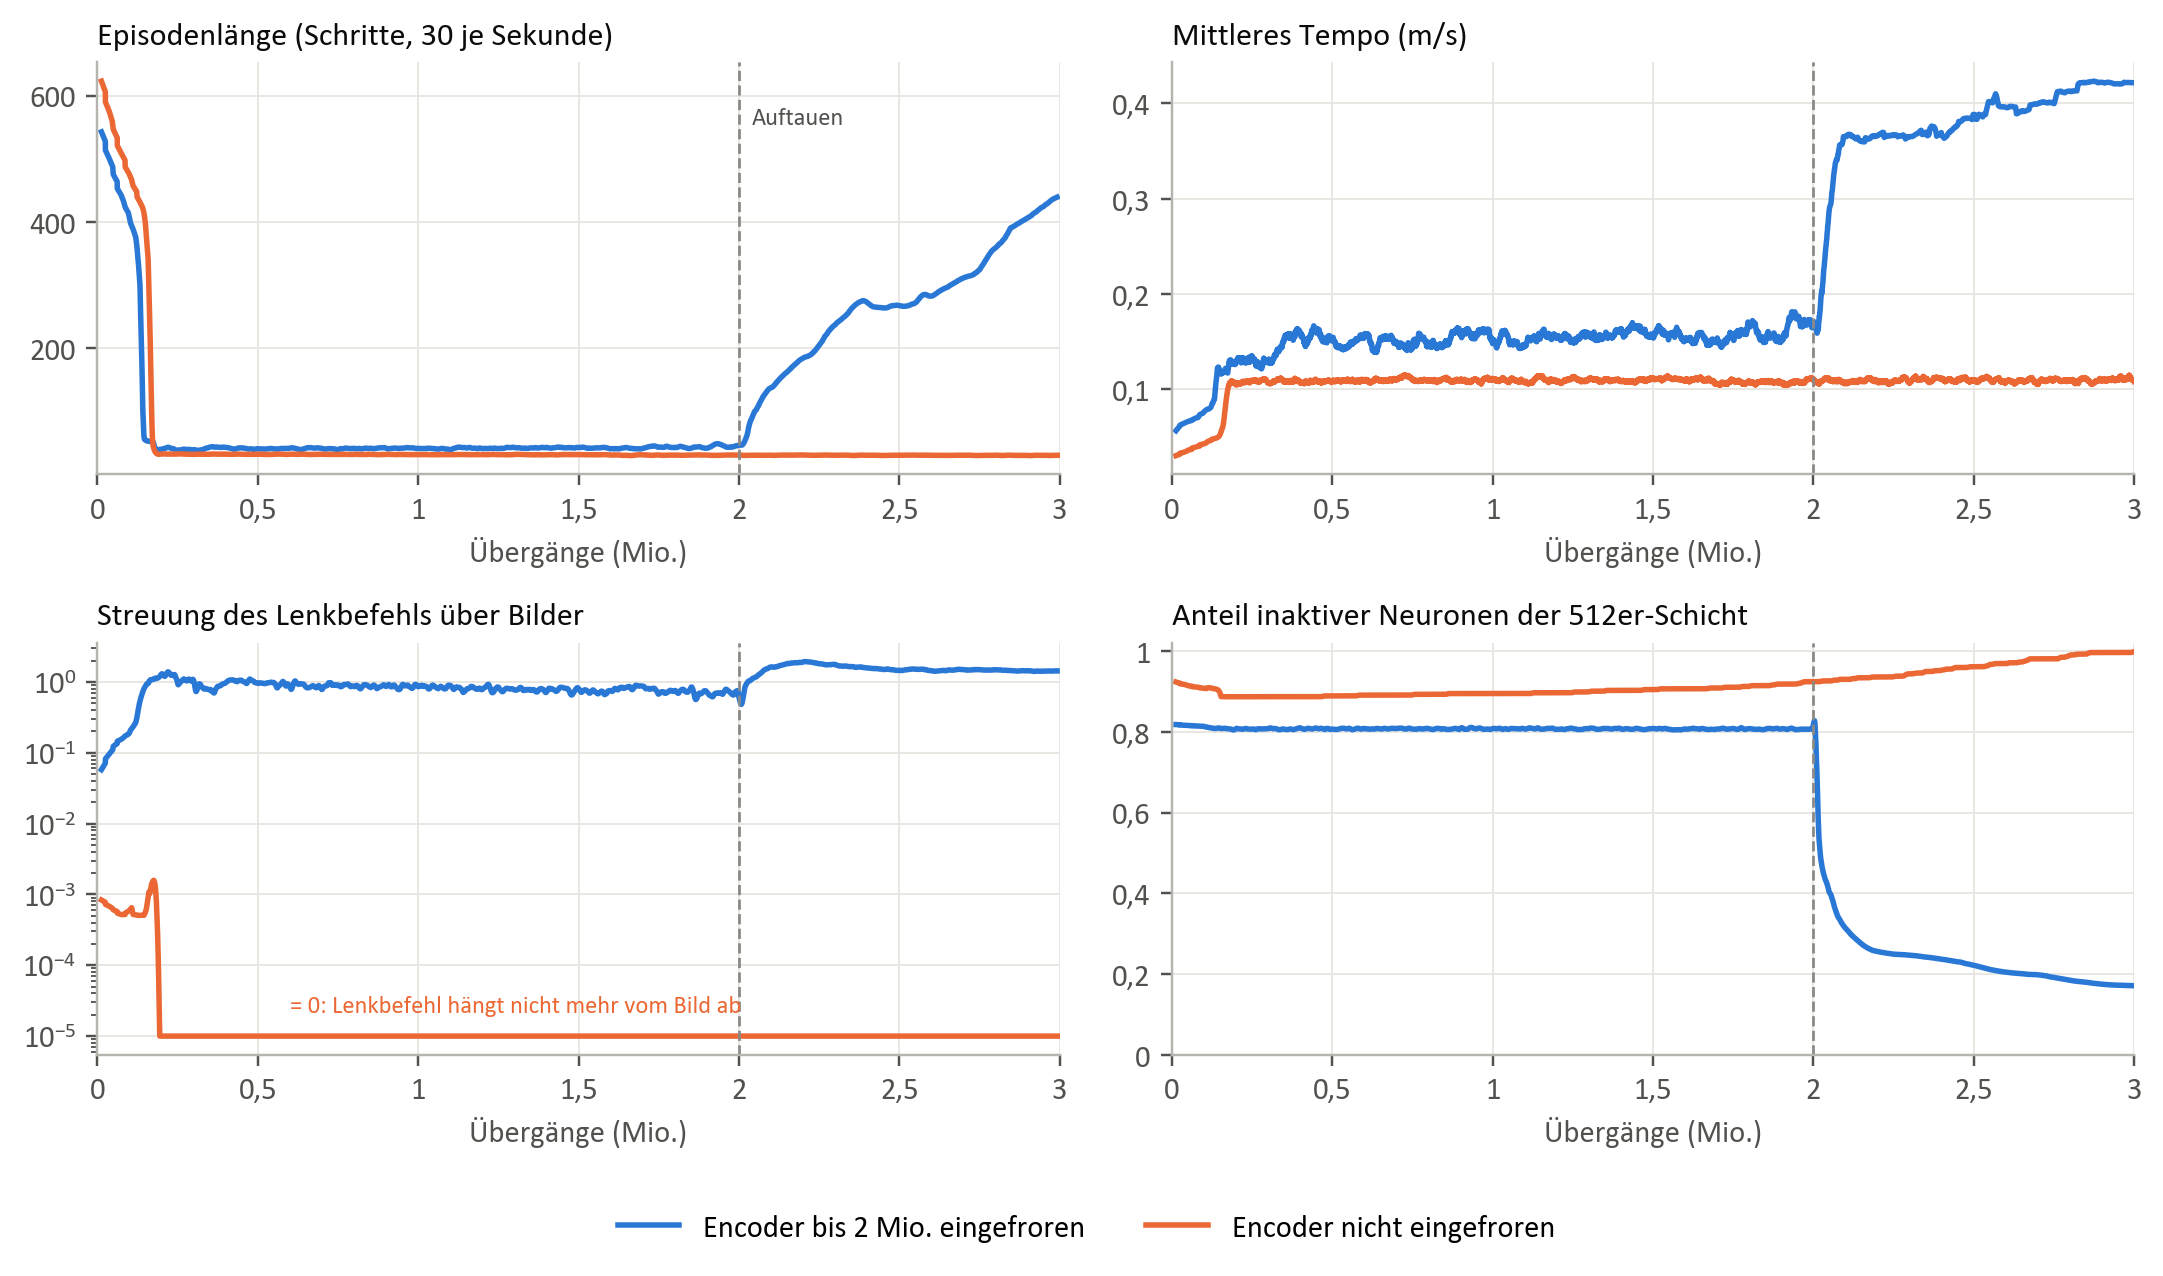
\includegraphics[width=\linewidth]{chapters/felix_teil/bilder/gegenversuch_einfrieren.png}
  \caption{Gegenversuch Einfrieren: identischer Aufbau mit eingefrorenem (blau) und nicht eingefrorenem Encoder (orange) auf \texttt{kurs\_A}.}
  \label{fig:gegenversuch_einfrieren}
\end{figure}

Ohne Einfrieren wird der Agent blind. Schon nach einer halben Million Übergängen hängt der Lenkbefehl nicht mehr vom Bild ab, und die 512er-Schicht stirbt bis zum Ende fast vollständig ab. Der Agent fährt keine Runde, die Episoden enden nach etwa einer Sekunde. Mit Einfrieren bleibt das Sehen erhalten; nach dem Auftauen steigen Episodenlänge und Tempo, und der Agent fährt nach \num{2.9}~Mio.\ Übergängen seine erste Runde.

Damit ist das Einfrieren als notwendig belegt. Ohne Schutz zerstört das \ac{RL} den vortrainierten Encoder in den ersten Hunderttausend Übergängen, bevor der Kopf gelernt hat, ihn zu nutzen.

\subsection{Der erste fahrende Kamera-Agent}
\label{sec:agent1}

Nach Behebung dieser Probleme gelingt mit Agent~1 das erste Training eines Kamera-Agenten, der zuverlässig Runden fährt.

\subsubsection{Genutzte Parameter}
\label{subsec:agent1_einstellungen}

Mit den Einstellungen aus Tabelle~\ref{tab:agent1_einstellungen} gelang das erste Training eines Kamera-Agenten, der zuverlässig Runden fährt.

Gegenüber den vorherigen Läufen wurden zwei Dinge geändert: Statt 64 laufen nur noch 4 parallele Umgebungen, wodurch der Erfahrungsspeicher je Umgebung 69 statt 4 Minuten Fahrt enthält, und die Faltungsschichten bleiben bis \num{0.3}~Mio.\ Übergänge eingefroren.

\begin{table}[htbp]
  \centering
  \caption{Einstellungen von Agent~1.}
  \label{tab:agent1_einstellungen}
  \small
  \begin{tabularx}{\linewidth}{@{}l X@{}}
    \toprule
    \textbf{Einstellung} & \textbf{Agent~1} \\
    \midrule
    Parallele Umgebungen                    & 4 \\
    Beobachtung                             & 3 Bilder à \num{250} $\times$ \num{150} Pixel, 256 Graustufen \\
    Darstellungen der Strecke               & 1 \\
    Vortraining                             & \ac{BC} auf \num{48000} Lehrerpaaren; übernommen: Faltungsschichten \\
    Eingefroren                             & Faltungsschichten bis \num{0.3}~Mio.\ Übergänge \\
    Batchgröße / Updates                    & 512 / 2 je Simulationsschritt (\num{0.5} je Übergang) \\
    Erfahrungsspeicher gesamt / je Umgebung & \num{500000} / \num{125000} Übergänge ($\approx$ \SI{69}{\minute} Fahrt) \\
    Lernrate / Diskontfaktor $\gamma$       & \num{5e-5} / \num{0.99} \\
    Episodenlänge                           & \SI{66.67}{\second}; in der Fortsetzung \SI{133.33}{\second} \\
    Übergänge im fertigen Modell            & \num{2.2}~Mio.\ (\num{1.2} + \num{1.0}) \\
    Durchsatz                               & $\approx$ 11 Übergänge/s (rund \SI{38}{\hour} je \num{1.5}~Mio.) \\
    \bottomrule
  \end{tabularx}
\end{table}

\subsubsection{Das Ergebnis}
\label{subsec:agent1_ergebnis}

Der erste erfolgreiche Agent fährt seine erste vollständige Runde nach rund \num{0.92}~Mio.\ Übergängen. Da das Training auf \num{1.5}~Mio.\ Übergänge ausgelegt ist und die Ergebnisse erstmals vielversprechend sind, wird es fortgesetzt: ausgehend vom Stand bei \num{1.2}~Mio.\ Übergängen um weitere \num{1.0}~Mio.\ Übergänge, mit doppelt so langen Episoden (\num{4000} statt \num{2000} Schritte). Längere Episoden setzen den Schwerpunkt auf stabiles Fahren, da der Agent mehr Runden am Stück fahren muss.

Dieser Agent lernt auf einer Strecke mit stets gleicher Darstellung. Abbildung~\ref{fig:agent1_verlauf} zeigt den Verlauf beider Trainingsabschnitte.

\begin{figure}[htbp]
  \centering
  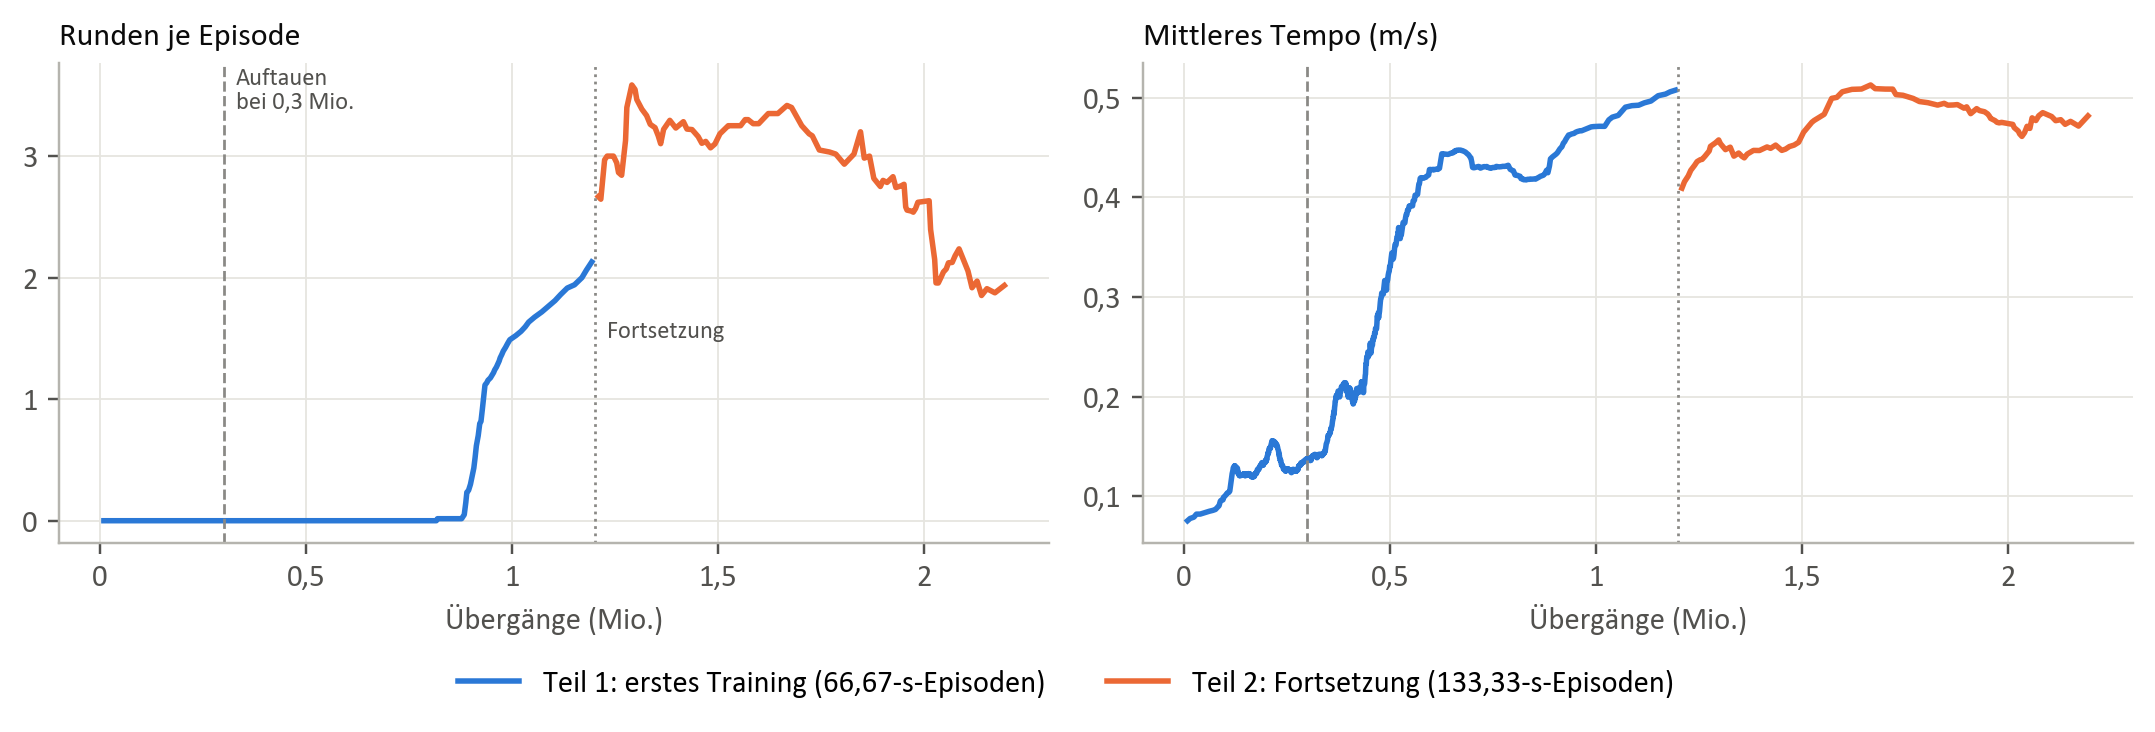
\includegraphics[width=\linewidth]{chapters/felix_teil/bilder/agent1_verlauf.png}
  \caption{Trainingsverlauf von Agent~1 (Werte mit Explorationsrauschen). Blau: erstes Training, orange: Fortsetzung mit doppelt so langen Episoden; gestrichelt: Auftauen der Faltungsschichten.}
  \label{fig:agent1_verlauf}
\end{figure}

Deterministisch gemessen, also ohne Explorationsrauschen und über zehn Episoden, fährt Agent~1 auf seiner Darstellung \num{6.4} Runden je Episode von \SI{66.67}{\second}, mit einer mittleren Geschwindigkeit von \SI{0.65}{\meter\per\second} und einer besten Runde von \SI{8.65}{\second}. Ca.\ \SI{10}{\percent} der Episoden enden mit einem Crash. Zum Vergleich fährt der zustandsbasierte Lehrer, der alle Größen exakt kennt, auf der gleichen Strecke etwa \SI{8.3}{\second} je Runde. Agent~1 ist also rund \SI{4}{\percent} langsamer, obwohl dieser die Lage und Bewegungen des Fahrzeugs aus \num{9} $\times$ \num{4} Pixeln ablesen muss. In Episoden von \SI{200}{\second} fährt er im Mittel \num{10.4} Runden mit einer besten Runde von \SI{8.59}{\second}. In 3 von 10 Episoden fährt er rund 20 Runden ohne Crash, \SI{70}{\percent} der langen Episoden enden jedoch vorzeitig. Der beste Bild-Agent der 2D-Umgebung schaffte unter vergleichbaren Bedingungen mit gestreuten Startpunkten \num{3.1} Runden.

Der kurze Einbruch zu Beginn der Fortsetzung in Abbildung~\ref{fig:agent1_verlauf} ist kein Verlernen. Stable-Baselines3 wählt in den ersten Schritten eines Laufs Zufallsaktionen, um den Speicher zu füllen; bei der Fortsetzung waren das \num{50000} Übergänge, in denen der Agent zufällig fuhr.

\paragraph{Ursache des Durchbruchs.}
Der Durchbruch dieses Agenten kann nicht eindeutig auf eine einzelne Änderung zurückgeführt werden. Gegenüber den vorherigen Läufen wird zum einen die Zahl der Umgebungen von 64 auf 4 reduziert, wodurch jede Umgebung einen größeren Anteil des Erfahrungsspeichers erhält, zum anderen werden erstmals die Faltungsschichten eingefroren. Damit wurde der Grundsatz verletzt, je Lauf nur eine Größe zu verändern.

Einen Hinweis liefert der vorherige Gegenversuch zum Einfrieren des Encoders (Abschnitt~\ref{sec:einfrieren}). Dort erblindet der Agent ohne Einfrieren, obwohl jede Umgebung mit \SI{104}{\minute} Fahrt über einen noch größeren Speicheranteil verfügt. Das spricht dafür, dass das Einfrieren den größeren Anteil am Durchbruch hatte. Für Agent~1 selbst ist es nicht belegt, da beide Änderungen nie getrennt untersucht wurden.

\subsubsection{Eine Einschränkung}
\label{subsec:agent1_einschraenkung}

Um zu prüfen, wie weit Agent~1 verallgemeinert, wurde er ohne weiteres Training auf derselben Streckenführung in anderen Darstellungen eingesetzt. Schon eine andere Darstellung genügt, damit er versagt. Auf jeder geprüften Darstellung fährt er null Runden, und jede Episode endet mit einem Crash, meist nach etwa einer Sekunde, ohne dass der Agent in Fahrt kommt. Das ist kein Fehler des Agenten, sondern eine Folge des Trainingsaufbaus. Über mehr als zwei Millionen Übergänge hinweg war das Kamerabild bis auf die Lage des Fahrzeugs identisch. Unter diesen Bedingungen ist Auswendiglernen die einfachste Lösung, und genau diese hat das Training gefunden.

Das deckt sich mit dem Befund aus Phase~1, dass bereits \SI{0.05}{\percent} abweichende Pixel eine Policy umwerfen können (Abschnitt~\ref{subsec:buffer}).

\subsection{Der zweite Agent}
\label{sec:agent2}

Dieser Abschnitt beschreibt den zweiten fahrenden Kamera-Agenten, im Folgenden Agent~2. Anders als Agent~1 soll er auch bei verändertem Aussehen der Strecke fahren. Dazu wechseln im Training die Darstellungen der Strecke, und der Encoder wird nicht auf die Aktionen eines Lehrers, sondern auf die Lage des Fahrzeugs vortrainiert.

\subsubsection{Verallgemeinern der Erscheinung}
\label{subsec:agent2_darstellung}

Das Problem von Agent~1 ist, dass er das Erscheinungsbild der Strecke und des Hintergrunds auswendig gelernt hat. Da der Agent auf einer realen Bahn fahren soll, muss dies behoben werden, da das reale Bild niemals exakt der Erscheinung der Simulation entsprechen wird. Untergrund, Licht, Unebenheiten und Farbunterschiede in der echten Strecke unterscheiden sich von der Simulation. Der Abstand zwischen der Darstellung im Training und der beim Einsatz heißt Domänenlücke (engl.\ \emph{domain gap}). Die übliche Abhilfe ist, im Training viele zufällig veränderte Darstellungen zu zeigen (\emph{Domain Randomization} \cite{tobin2017domain}).

Für die Randomisierung wurde ein Streckengenerator entwickelt, der Strecken aus Bildern der realen Carrera-Streckenteile zusammensetzt. Damit werden für dieselbe Streckenführung zwölf Darstellungen erzeugt, drei Untergründe kombiniert mit vier Helligkeitsstufen der Fahrbahn (Abbildung~\ref{fig:darstellungen}). Derselbe Generator erzeugt auch neue Streckenführungen, die in Abschnitt~\ref{sec:andere_strecken} verwendet werden.

\begin{figure}[htbp]
  \centering
  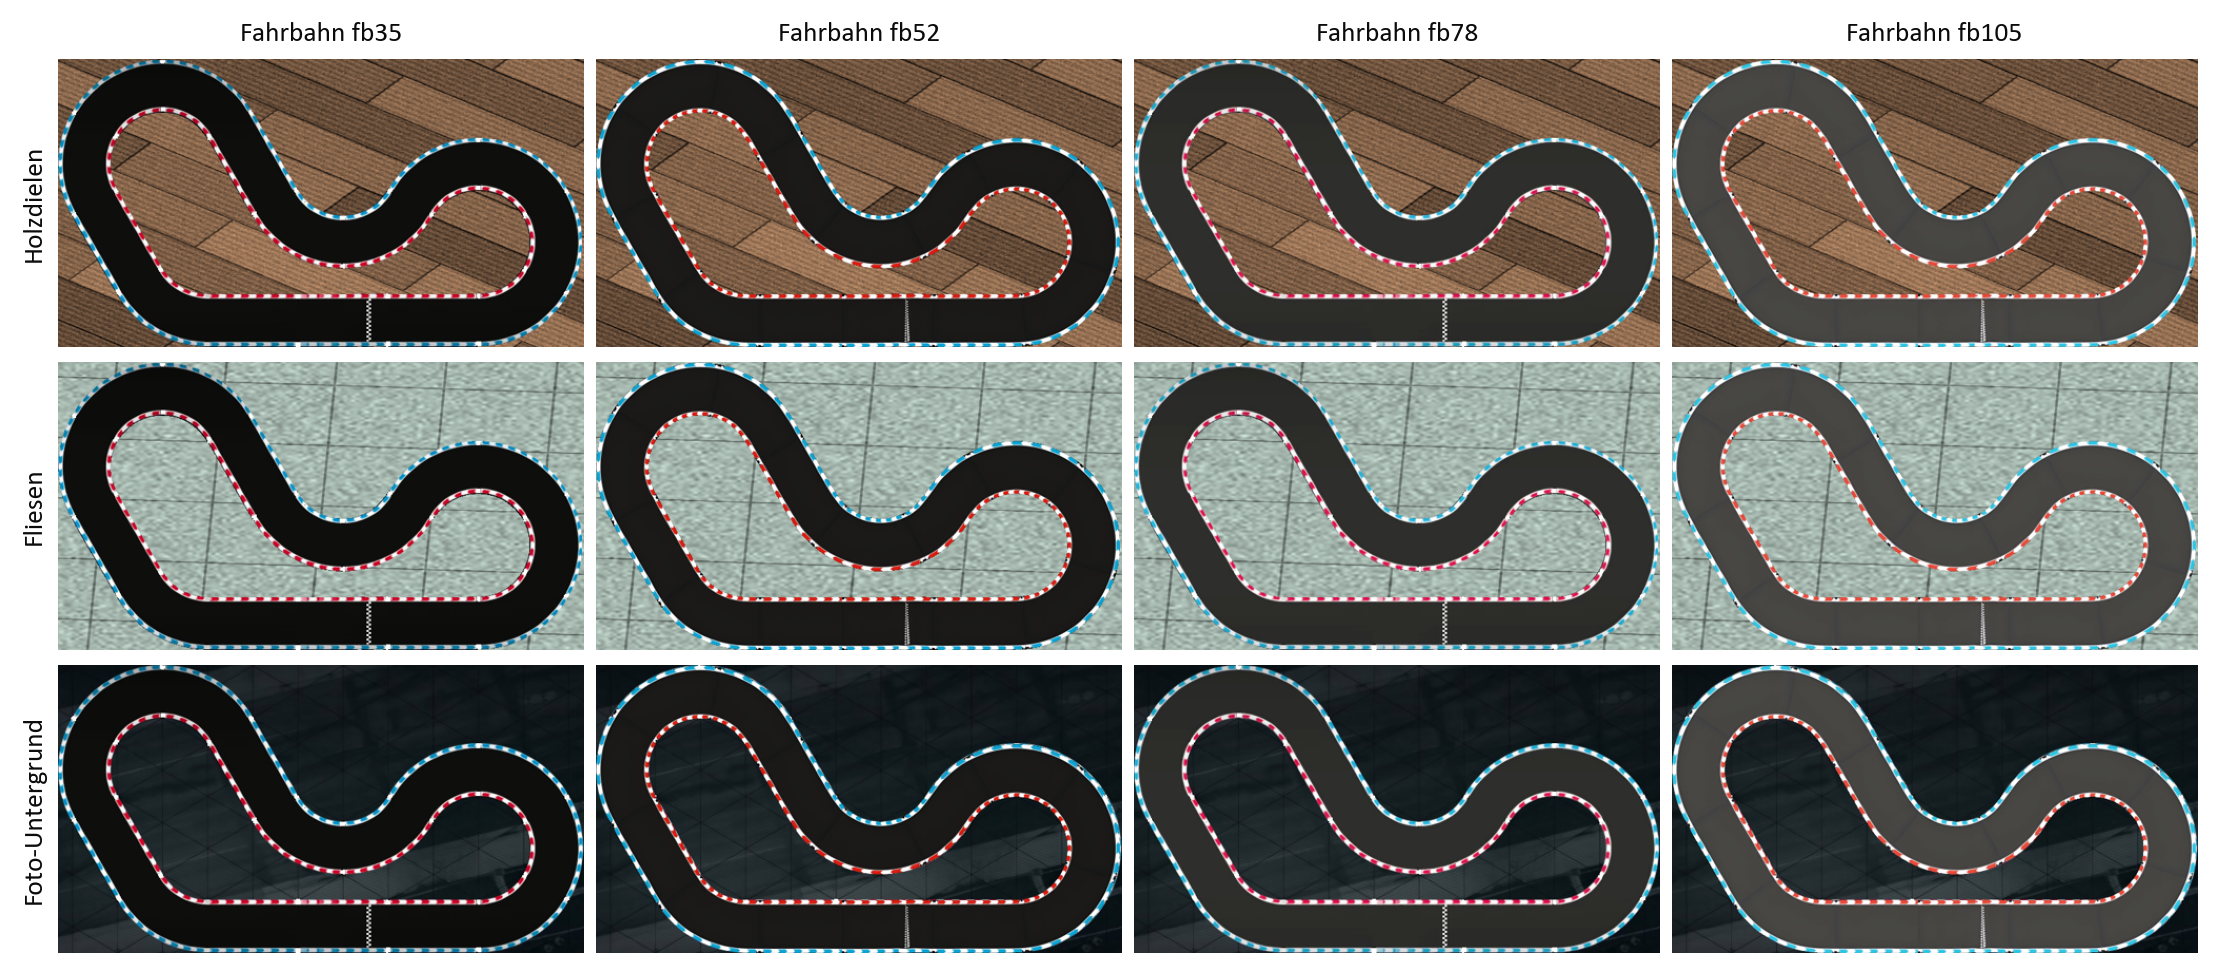
\includegraphics[width=\linewidth]{chapters/felix_teil/bilder/darstellungen.png}
  \caption{Die zwölf Darstellungen der Trainingsstrecke: drei Untergründe (Zeilen) und vier Helligkeiten der Fahrbahn (Spalten).}
  \label{fig:darstellungen}
\end{figure}

Weiterhin wird das Bild für Agent~2 auf vier Graustufen reduziert. Feine Unterschiede der Oberflächen verschwinden dadurch weitgehend, während Fahrbahn, Randsteine und Fahrzeug unterscheidbar bleiben. Zugleich lassen sich die Bilder mit \SI{2}{\bit} je Pixel im Erfahrungsspeicher ablegen.

\subsubsection{Das Training}
\label{subsec:agent2_training}

Agent~2 wird mit 16 parallelen Umgebungen trainiert. Der vortrainierte Encoder wird vollständig übernommen und bleibt bis 2~Mio.\ Übergänge eingefroren. Seine erste vollständige Runde fährt der Agent nach \num{3.9}~Mio.\ Übergängen. Das fertige Modell wurde über \num{14.5}~Mio.\ Übergänge in rund \SI{92}{\hour} trainiert.

Abbildung~\ref{fig:agent2_verlauf} zeigt den Trainingsverlauf. Die Kurven enthalten das Explorationsrauschen und sind über alle Darstellungen gemittelt. Sie liegen daher deutlich unter den deterministisch gemessenen Werten. Zwischen \num{4.4} und 5~Mio.\ Übergängen stieg der Verlust des Critics um das Hundertfache, und das Fahren brach vorübergehend ein. Zeitlich fällt das mit den ersten Runden zusammen, deren Bonus die Zielwerte des Critics sprunghaft erhöht. Der Encoder blieb dabei intakt, und der Agent erholte sich ohne Eingriff. Das ist ein Hinweis zu der in Phase~1 offenen Frage, warum \ac{SAC}-Läufe nach ihrem Höhepunkt einbrechen (Abschnitt~\ref{subsec:ppo_sac_vergleich}), aber keine Erklärung.

\begin{figure}[htbp]
  \centering
  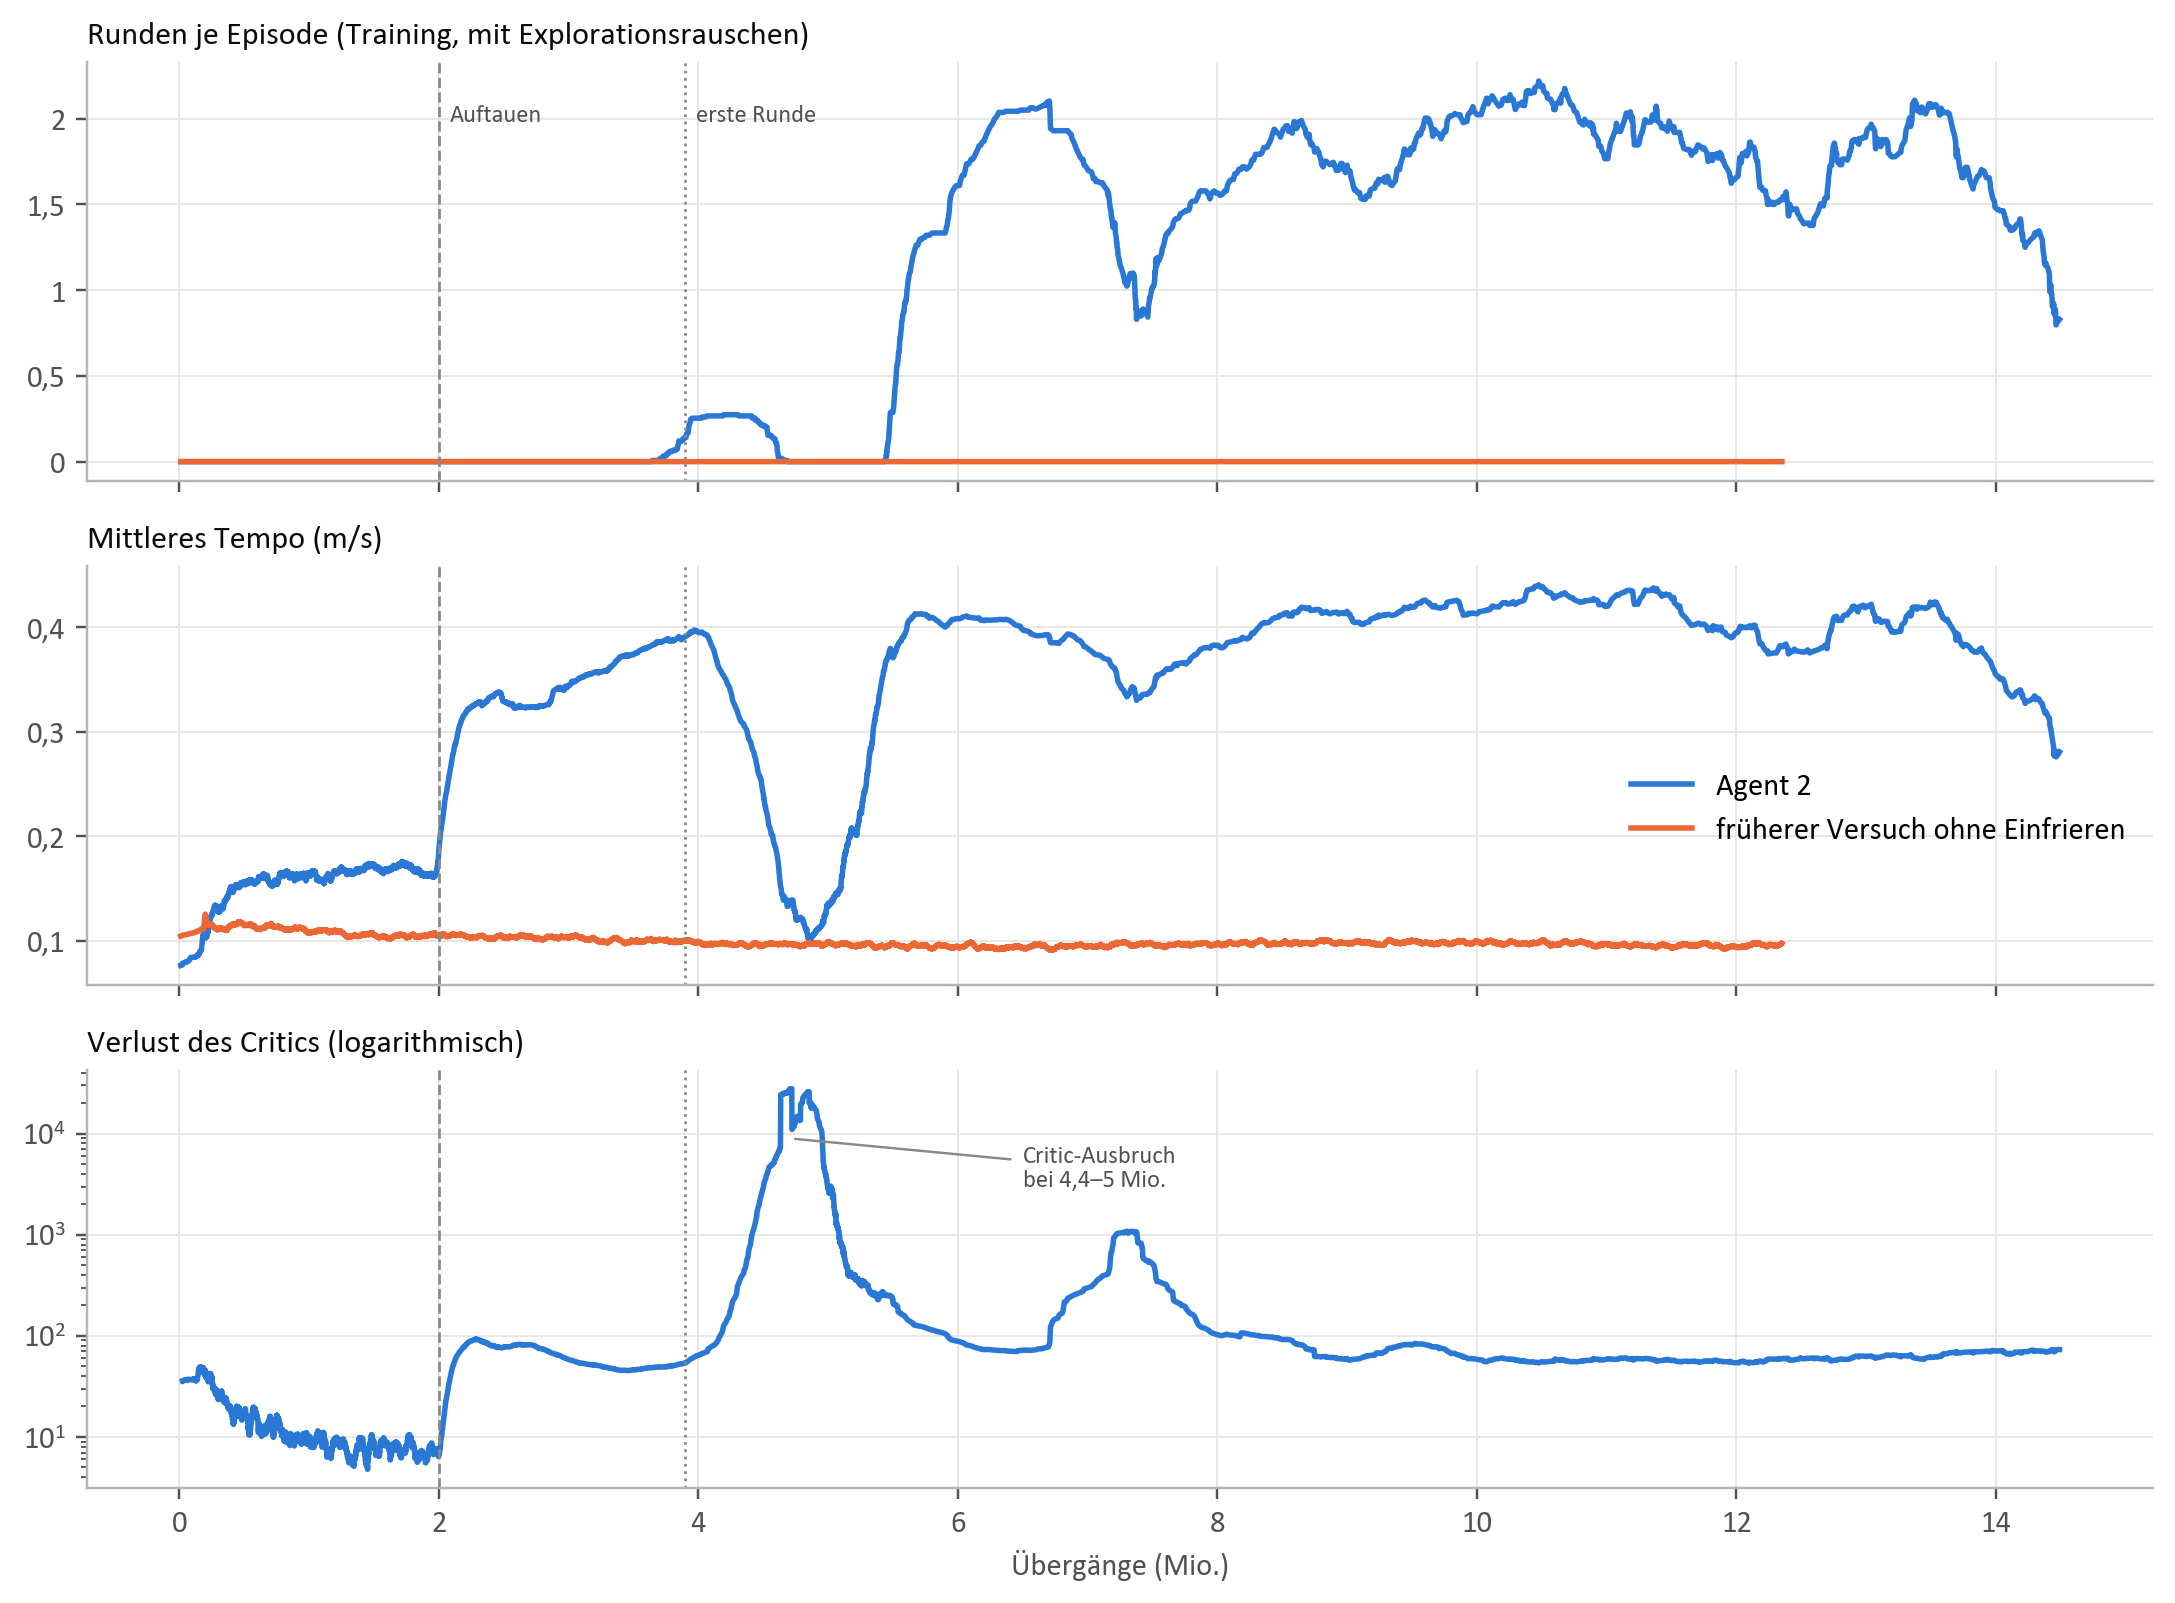
\includegraphics[width=\linewidth]{chapters/felix_teil/bilder/agent2_verlauf.png}
  \caption{Trainingsverlauf von Agent~2 im Vergleich zu einem früheren Versuch ohne Einfrieren (Werte mit Explorationsrauschen). Gestrichelt: Auftauen; gepunktet: erste vollständige Runde.}
  \label{fig:agent2_verlauf}
\end{figure}

\subsubsection{Das Ergebnis}
\label{subsec:agent2_ergebnis}

Abbildung~\ref{fig:agent2_darstellungen} zeigt das Ergebnis von Agent~2 nach \num{14.5}~Mio.\ Übergängen auf allen zwölf Darstellungen. Im Mittel fährt er \num{4.5} Runden je Episode bei einem Tempo von \SI{0.53}{\meter\per\second}. Die beste Runde dauert \SI{9.65}{\second}, und \SI{31}{\percent} der Episoden enden mit einem Crash. Auf allen zwölf Darstellungen fährt er Runden, auf sieben davon im Mittel mindestens fünf.

\begin{figure}[htbp]
  \centering
  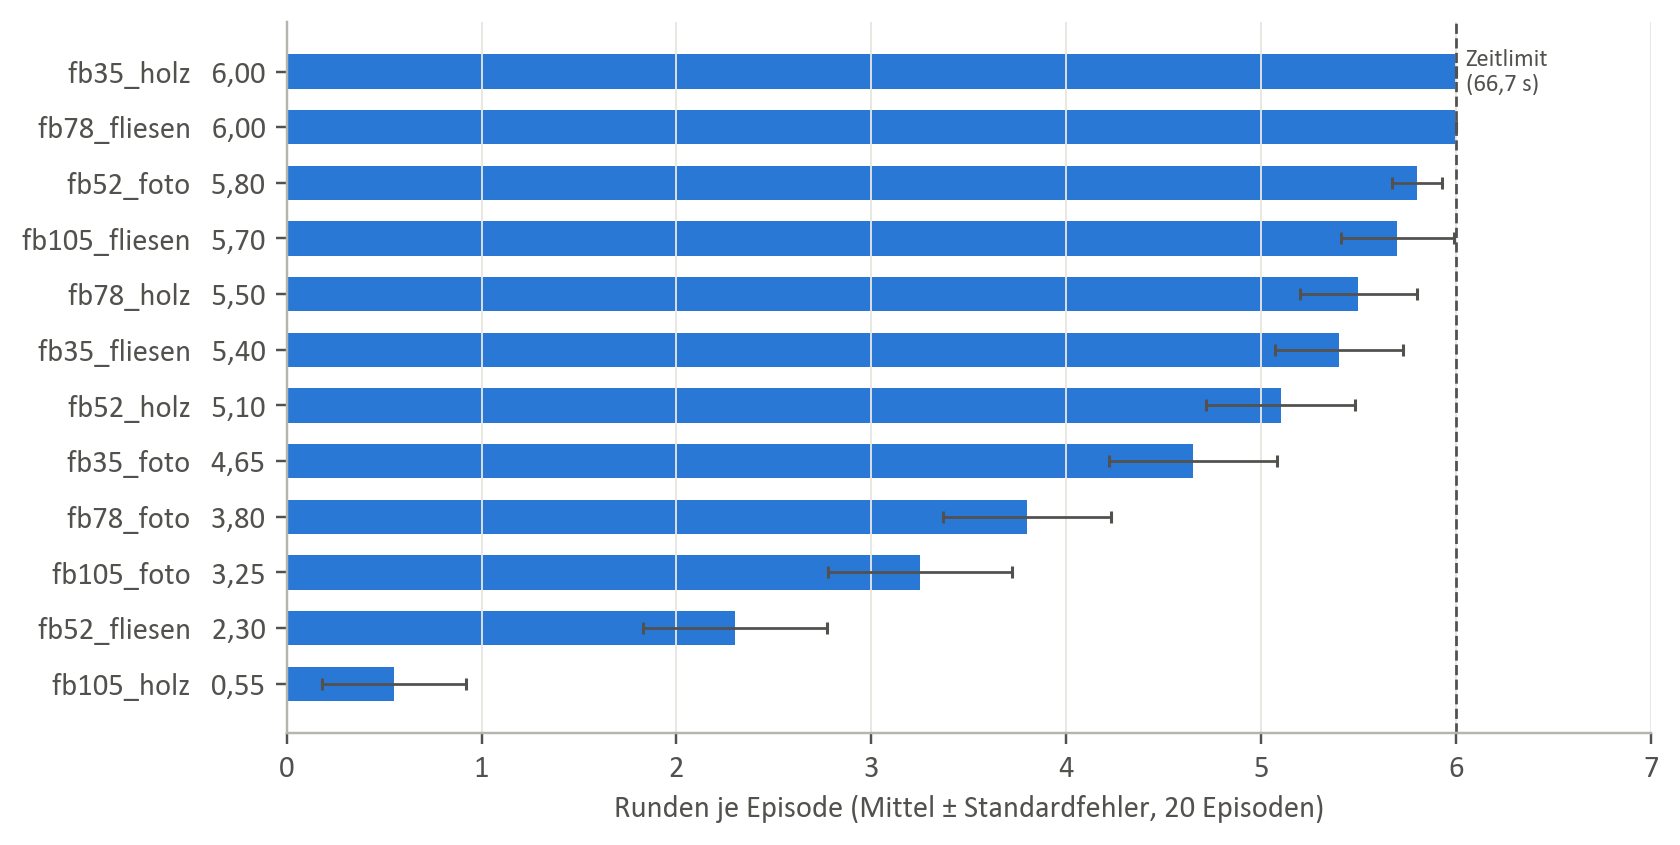
\includegraphics[width=0.9\linewidth]{chapters/felix_teil/bilder/agent2_darstellungen.png}
  \caption{Agent~2 auf den zwölf Darstellungen (je 20 Episoden à \SI{66.67}{\second}, deterministisch). Bei 6 Runden liegt das Zeitlimit. Die Werte der unteren Darstellungen sind Grenzfälle und schwanken zwischen Messungen; für \texttt{fb105\_holz} lagen sie in verschiedenen Messungen zwischen 0 und 4 Runden.}
  \label{fig:agent2_darstellungen}
\end{figure}

Drei Darstellungen erreichen bei \SI{66.67}{\second} das Zeitlimit von sechs Runden in jeder Episode, die Messung zeigt dort also nicht das Können, sondern die Episodenlänge. Mit \SI{200}{\second} langen Episoden fährt Agent~2 auf diesen drei Darstellungen \num{19} bis \num{19.7} Runden ohne einen einzigen Crash, im Mittel über alle zwölf \num{12.4} Runden.

\paragraph{Gegenprobe mit Agent~1.}
Als Gegenprobe wurde Agent~1 auf denselben zwölf Darstellungen gemessen: Er fährt auf keiner einzigen eine Runde und verlässt nach etwa einer Sekunde die Fahrbahn. Die Verallgemeinerung von Agent~2 ist damit nicht nur behauptet, sondern gegen ein Modell ohne Randomisierung geprüft.

\paragraph{Wo die schwachen Darstellungen scheitern.}
Auf den Darstellungen mit vielen Crashes verlässt der Agent fast immer in derselben Kurve die Fahrbahn. Der Hergang ist jedes Mal gleich: Innerhalb von \SI{0.3}{\second} wächst der Richtungsfehler von nahezu null auf über \SI{30}{\degree}, und der Gegenlenkbefehl kommt zu spät. Das Tempo ist dabei nicht die Ursache; auf einer sicher gefahrenen Darstellung durchfährt er dieselbe Kurve sogar schneller. Auch die Sichtbarkeit ist es nicht: Der Encoder liest die Lage auf der schwächsten Darstellung genauer ab als auf mancher sicher gefahrenen. Der Agent hat an dieser Stelle schlicht eine sehr kleine Reserve, sodass jede kleine Änderung der Eingabe das Ergebnis umkippen kann.

\paragraph{Feinere Graustufen.}
Dazu passt ein überraschender Befund. Wird das Kamerabild bei der Messung auf acht statt auf die trainierten vier Graustufen reduziert, sinkt die Crashrate auf der Darstellung \texttt{fb52\_fliesen} von \SI{80}{\percent} auf \SI{0}{\percent}, ohne jedes Nachtraining, auch mit 16 und 256 Stufen gab es keinen Crash. Der Agent verträgt also feinere Eingaben als die, auf denen er trainiert wurde. Für die Übertragung auf eine echte Kamera mit 256 Graustufen ist das die günstige Richtung.

\paragraph{Lohnt sich das lange Training?}
Agent~2 wurde nach \num{6.5} und nach \num{14.5}~Mio.\ Übergängen gemessen. Die Differenz von \num{0.54} Runden je Episode liegt innerhalb der Messunsicherheit (Standardfehler \num{0.61}), und die spätere Fassung ist nur auf sieben von zwölf Darstellungen besser. Sicher nachweisbar ist nur, dass sie schneller fährt, auf allen zwölf Darstellungen, mit kürzeren Rundenzeiten. Die zweite Hälfte des Trainings, rund \SI{50}{\hour}, hat also im Wesentlichen das Tempo verbessert, nicht die Zuverlässigkeit.

\subsection{Vergleich der beiden Modelle}
\label{sec:agentenvergleich}

Tabelle~\ref{tab:agentenvergleich} stellt Agent~1 und Agent~2 gegenüber. Die beiden Modelle lösen verschiedene Aufgaben und sind deshalb nicht direkt vergleichbar. Agent~1 fährt auf einer Darstellung und ist auf diese spezialisiert. Agent~2 dagegen fährt auf 12 unterschiedlichen Darstellungen.

\begin{table}[htbp]
  \centering
  \caption{Die beiden fahrenden Kamera-Agenten.}
  \label{tab:agentenvergleich}
  \small
  \begin{tabularx}{\linewidth}{@{}l X X@{}}
    \toprule
     & \textbf{Agent~1} & \textbf{Agent~2} \\
    \midrule
    Aufgabe                          & 1 Darstellung & 12 Darstellungen mit Bildstörungen \\
    Vortraining                      & \ac{BC} eines Lehrers (Fahrwissen) & Encoder für Versatz und Richtung (nur Sehwissen) \\
    Eingefroren                      & Faltungen bis \num{0.3}~Mio.\ Übergänge & gesamter Encoder bis 2~Mio.\ Übergänge \\
    Parallele Umgebungen             & 4 & 16 \\
    Graustufen                       & 256 & 4 \\
    Speicher je Umgebung             & \SI{69}{\minute} Fahrt & \SI{104}{\minute} Fahrt \\
    Übergänge bis zur ersten Runde   & \num{0.92}~Mio. & \num{3.9}~Mio. \\
    Übergänge im fertigen Modell     & \num{2.2}~Mio. & \num{14.5}~Mio. \\
    Runden je Episode (\SI{66.67}{\second}) & \num{6.4} auf seiner Darstellung, 0 auf den 12 anderen & \num{4.5} im Mittel über 12 \\
    Beste Runde                      & \SI{8.65}{\second} & \SI{9.65}{\second} \\
    Episoden mit Crash               & \SI{10}{\percent} & \SI{31}{\percent} \\
    \bottomrule
  \end{tabularx}
\end{table}

Neben der Aufgabe unterscheiden sich die beiden Agenten vor allem im Vortraining. Agent~1 hat Fahrwissen vom Lehrer geerbt, Agent~2 hat nur gelernt, wo das Auto auf der Bahn liegt, und das Fahren vollständig selbst gelernt. Dass Agent~2 viermal so viele Übergänge bis zur ersten Runde braucht, ist vor diesem Hintergrund und bei zwölffacher Aufgabe nicht überraschend.

\subsection{Test des zweiten Agenten auf anderen Streckenführungen}
\label{sec:andere_strecken}

Agent~2 fährt auf allen zwölf Darstellungen der Trainingsstrecke. Offen ist, ob er damit das Fahren an sich gelernt hat oder nur diese eine Streckenführung. Dazu wird er zunächst ohne weiteres Training auf neuen Streckenführungen getestet und anschließend auf zwei davon weitertrainiert.

\subsubsection{Test ohne Nachtraining}
\label{subsec:ohne_nachtraining}

Agent~2 wird ohne weiteres Training auf vier neuen Streckenführungen (\texttt{kurs\_A} bis \texttt{kurs\_D}) getestet, die mit dem Streckengenerator aus Abschnitt~\ref{subsec:agent2_darstellung} erzeugt wurden. Damit sich nur die Führung verändert und nicht gleichzeitig das Aussehen, wurden für \texttt{kurs\_A} dieselben zwölf Darstellungen erzeugt, auf denen Agent~2 trainiert wurde (Tabelle~\ref{tab:ohne_nachtraining}).

\begin{table}[htbp]
  \centering
  \caption{Agent~2 ohne Nachtraining (deterministisch).}
  \label{tab:ohne_nachtraining}
  \small
  \begin{tabular}{@{}l l l@{}}
    \toprule
    \textbf{Strecke} & \textbf{Darstellung} & \textbf{Runden je Episode} \\
    \midrule
    Original                              & trainiert (12) & \num{4.5} (\SI{66.67}{\second}) bzw.\ \num{12.4} (\SI{200}{\second}) \\
    Original                              & unbekannt      & \num{2.3} \\
    \texttt{kurs\_A}                      & trainiert (12) & \num{0.00} auf allen 12 \\
    \texttt{kurs\_A} bis \texttt{kurs\_D} & unbekannt      & \num{0.00} \\
    \bottomrule
  \end{tabular}
\end{table}

Eine unbekannte Darstellung der bekannten Strecke fährt der Agent noch mit \num{2.3} Runden. Eine unbekannte Streckenführung fährt er dagegen nicht, auch wenn sie in den bekannten Darstellungen gezeigt wird. Sein Verhalten auf \texttt{kurs\_A} ist dabei kein schlechteres Fahren, sondern eine Sättigung, voller Lenkeinschlag, Vollgas und Vollbremse gleichzeitig, ohne jede Korrektur. Es ist dasselbe Muster wie bei den blinden Agenten, obwohl der Encoder hier intakt ist.

Besonders aufschlussreich ist, dass \texttt{kurs\_A} die um \SI{180}{\degree} gedrehte Originalstrecke ist. Der Agent hat also nicht die Form der Strecke gelernt, sondern die Form in dieser Lage im Kamerabild. Für eine fest montierte Kamera über einer festen Strecke ist das kein Nachteil. Ein Agent, der jede beliebige Strecke fährt, entsteht so aber nicht.

\subsubsection{Weitertrainieren von Agent~2 gegen Neustart}
\label{subsec:weitertrainieren}

Da Agent~2 neue Streckenführungen ohne weiteres Training nicht fährt, wird untersucht, ob sein Vorwissen das Erlernen einer neuen Strecke zumindest beschleunigt. Dazu wird auf zwei Streckenführungen jeweils ein Weitertraining von Agent~2 mit einem Neustart verglichen:

\begin{description}
  \item[Weitertraining:] ausgehend vom fertigen Agent~2, also mit seinem Encoder und seiner Fahrweise;
  \item[Neustart:] ein neuer Agent mit demselben vortrainierten Encoder wie zu Beginn von Agent~2, eingefroren bis 2~Mio.\ Übergänge.
\end{description}

Als Strecken dienen \texttt{kurs\_A}, die gedrehte Originalstrecke, und \texttt{kurs\_D}, deren Fahrbahnfläche sich im Kamerabild nur zu \SI{21}{\percent} mit der Originalstrecke deckt. Gemessen wurde, nach wie vielen Übergängen die erste vollständige Runde fällt (Tabelle~\ref{tab:transfer}, Abbildung~\ref{fig:transfer}).

\begin{table}[htbp]
  \centering
  \caption{Übergänge bis zur ersten vollständigen Runde.}
  \label{tab:transfer}
  \small
  \begin{tabularx}{\linewidth}{@{}X l l l@{}}
    \toprule
    \textbf{Strecke} & \textbf{Weitertraining} & \textbf{Neustart} & \textbf{Ersparnis} \\
     & \textbf{(von Agent~2)} & \textbf{(nur Encoder)} & \\
    \midrule
    \texttt{kurs\_A} (Original, um \SI{180}{\degree} gedreht) & \num{2.81}~Mio. & \num{2.90}~Mio. & \SI{3}{\percent} \\
    \texttt{kurs\_D} (unähnlichste Führung)                   & \num{2.92}~Mio. & \num{3.29}~Mio. & \SI{11}{\percent} \\
    zum Vergleich: Agent~2 auf der Originalstrecke            & --              & \num{3.90}~Mio. & -- \\
    \bottomrule
  \end{tabularx}
\end{table}

\begin{figure}[htbp]
  \centering
  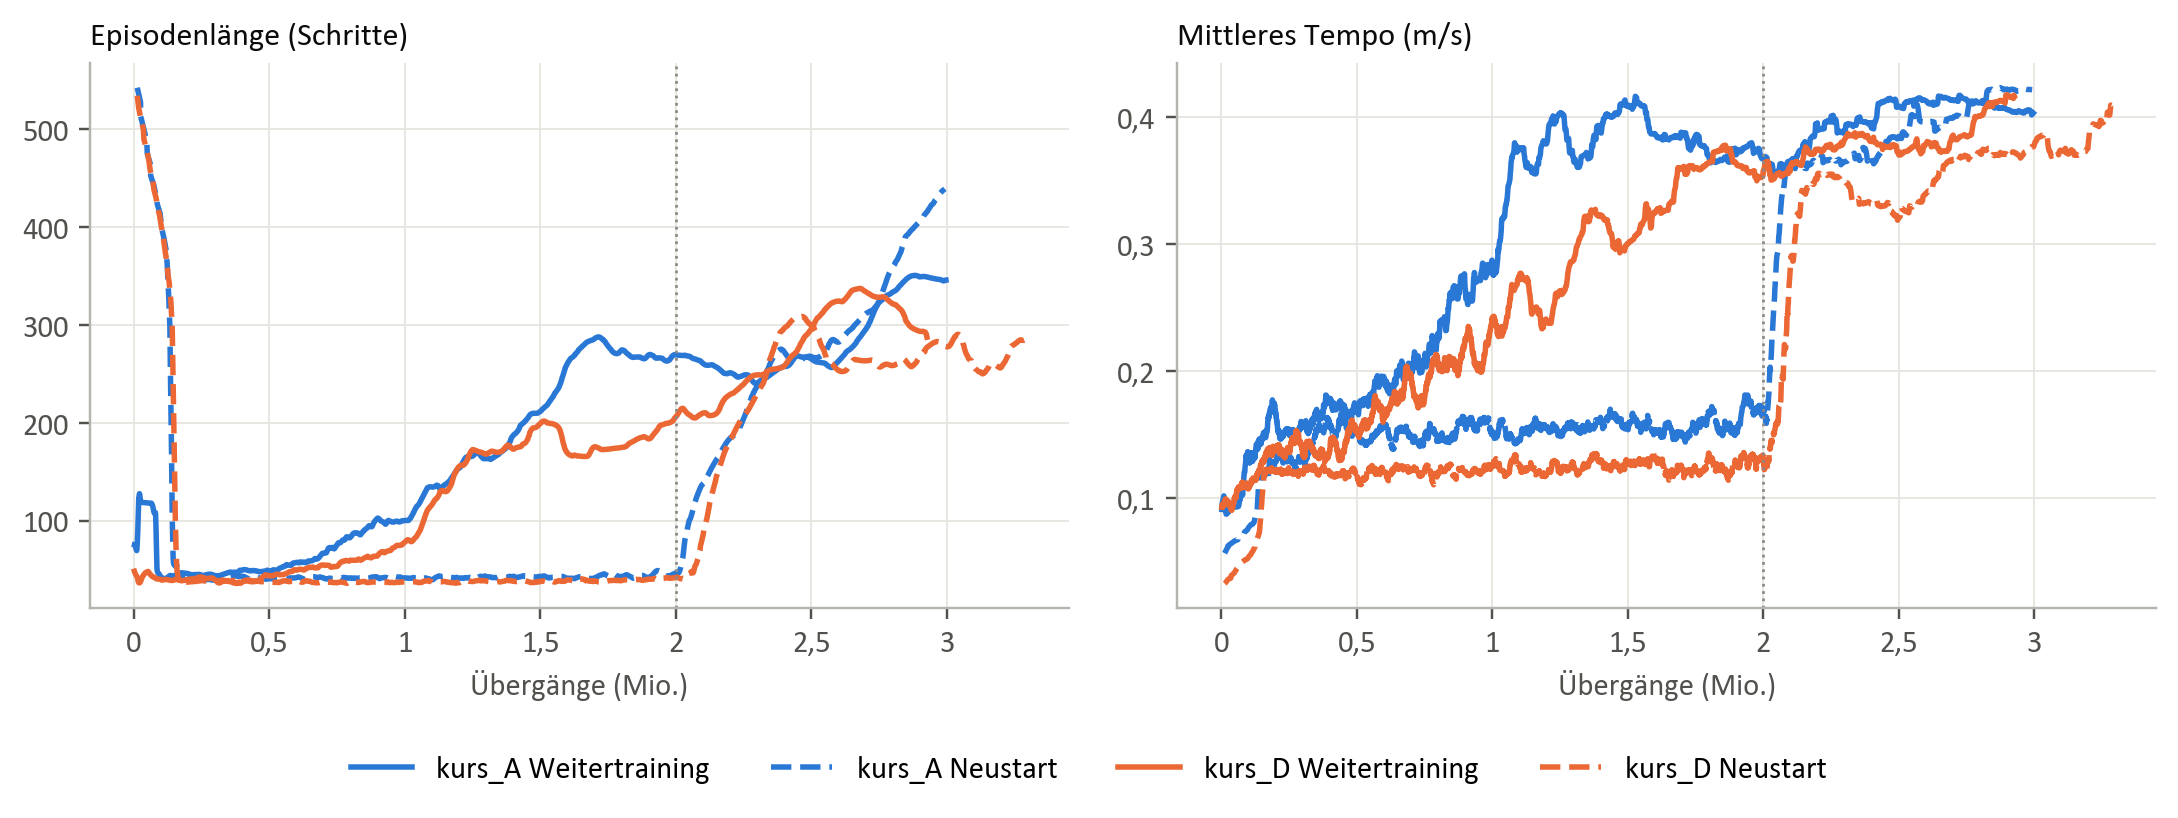
\includegraphics[width=\linewidth]{chapters/felix_teil/bilder/transfer.png}
  \caption{Weitertrainieren (durchgezogen) gegen Neustart (gestrichelt) auf \texttt{kurs\_A} (blau) und \texttt{kurs\_D} (orange). Bei 2~Mio.\ Übergängen wird der Encoder der Neustarts aufgetaut.}
  \label{fig:transfer}
\end{figure}

Das Vorwissen aus dem Training von Agent~2 bringt wenig: \SI{3}{\percent} auf \texttt{kurs\_A} und \SI{11}{\percent} auf \texttt{kurs\_D}. Da je Bedingung nur ein Lauf gefahren wird, kann ein Unterschied von \SI{3}{\percent} auch zufällig entstehen. Abbildung~\ref{fig:transfer} zeigt, woher der Unterschied kommt. Der weitertrainierte Agent lernt von Beginn an, weil sein Encoder nicht eingefroren werden muss, und ist nach \num{600000} bis \num{800000} Übergängen deutlich weiter. Sobald der Encoder des neu gestarteten Agenten bei 2~Mio.\ Übergängen aufgetaut wird, holt dieser den Rückstand innerhalb von etwa \num{600000} Übergängen auf.

Übertragbar ist damit das \emph{Sehen}, also die Fähigkeit, die Lage des Fahrzeugs im Bild abzulesen. Die \emph{Fahrweise} ist nicht übertragbar. Der Agent lernt nicht das allgemeine Fahren, sondern diese eine Strecke in dieser einen Kameraansicht.

Zwei Einschränkungen gelten für diesen Vergleich. Zum einen wird der Encoder des neu gestarteten Agenten auf Bildern der Originalstrecke trainiert. Beide Bedingungen bringen also Vorwissen von der Originalstrecke mit, und gemessen wurde genau der Beitrag der Fahrweise. Wie viel der Encoder auf einer fremden Strecke beiträgt, wurde nicht gemessen. Ein Neustart ganz ohne Encoder wurde dort nicht gefahren. Zum anderen musste der Neustart auf \texttt{kurs\_D} ab 3~Mio.\ Übergängen mit leerem Erfahrungsspeicher fortgesetzt werden, weil sich der gesicherte Speicher nicht laden ließ. Das hat ihn vermutlich gebremst; die \SI{11}{\percent} sind daher eher eine Obergrenze.
  % Felix: Phase 2, Trainingsablauf
% 04-ergebnisse.tex
\chapter{Ergebnisse}
\label{chap:ergebnisse}

Das wesentliche Ergebnis der 2D-Untersuchungen ist keine einzelne Zahl, sondern eine \emph{Pipeline}: eine Abfolge von Arbeitsschritten, mit der sich komplexere Agenten trainieren lassen, und die zugehörigen Prüfkriterien, an denen jeder Schritt gemessen wird. Dieses Kapitel stellt zunächst diese Pipeline in ihrem aktuellen Stand dar, belegt sie anschließend mit den gemessenen Werten und bewertet abschließend ihre Übertragbarkeit in die 3D-Simulation.

\section{Die aktuelle Trainingspipeline}
\label{sec:ergebnisse_pipeline}

Die Pipeline gliedert sich in vier Stufen. Entscheidend ist nicht nur ihre Reihenfolge, sondern dass jede Stufe eine eigene, unabhängig prüfbare Aussage liefert -- so lässt sich ein Fehlschlag eindeutig zuordnen, statt die gesamte Kette in Frage zu stellen.

\paragraph{Stufe 1 -- Privilegierter Lehrer-Agent.}
Ein zweischichtiges \ac{MLP} wird mit \ac{PPO} auf der vierdimensionalen Raycast-Beobachtung nach Gleichung~\eqref{eq:lidar_obs} trainiert. Der Agent konvergiert in rund zwölf Minuten und fährt anschließend elf fehlerfreie Runden bei einem Durchschnittstempo von etwa \SI{1.2}{\meter\per\second}.

\emph{Prüfkriterium:} Erreicht der Lehrer die volle Episodenlänge ohne Crash, sind Physik, Belohnungsfunktion, Streckengeometrie und Trainingspipeline lösbar. Erst dann ist eine Kameravariante sinnvoll.

\paragraph{Stufe 2 -- Datenaufzeichnung mit Rausch-Injektion.}
Der Lehrer fährt die Strecke unter additivem gaußschem Rauschen auf seine Aktionen (Gleichung~\eqref{eq:noise}). Das Fahrzeug driftet dadurch von der Ideallinie ab, und der Lehrer muss aktiv gegensteuern. Aufgezeichnet werden Paare aus visuellem Dreierstapel und der \emph{unverrauschten} Korrekturaktion. Der Datensatz enthält dadurch Rettungsmanöver, die eine perfekte Vorführung nie erzeugen würde.

\emph{Prüfkriterium:} Der Datensatz muss Zustände abseits der Ideallinie enthalten; ein Datensatz ohne Abweichungen erzeugt einen Schüler, der beim ersten eigenen Fehler ausfällt.

\paragraph{Stufe 3 -- Visuelles Vortraining.}
Ein \ac{CNN} lernt überwacht, die Expertenaktionen aus dem Bildstapel vorherzusagen (Gleichung~\eqref{eq:bc}). Erreicht wird ein MSE von \num{0.0034}. Übertragen werden anschließend ausschließlich die drei Faltungsschichten; die Linear-Schichten werden verworfen.

\emph{Prüfkriterium:} Hier ist besondere Vorsicht geboten. Ein niedriger MSE belegt \emph{nicht}, dass das Netz fahren kann -- in diesem Projekt fuhr kein einziges vortrainiertes Netz eigenständig mehr als \num{230} Frames. Was der Schritt liefert, ist Sehfähigkeit, nicht Fahrwissen. Ob er seinen Aufwand rechtfertigt, ist für \ac{SAC} bis heute nicht belegt (Abschnitt~\ref{subsec:vortraining}).

\paragraph{Stufe 4 -- Online-Feintuning mit SAC.}
Der so initialisierte Agent wird mit \ac{SAC} auf der Bildbeobachtung weitertrainiert. Maßgeblich sind dabei die in Tabelle~\ref{tab:pipeline_config} zusammengefassten Einstellungen; sie stammen aus dem aktuellsten großen Trainingslauf und sind die Konfiguration, die für Phase~2 übernommen werden soll.

\begin{table}[htbp]
  \centering
  \caption{Konfiguration der aktuellen Pipeline-Stufe~4, entnommen aus \texttt{train\_config.json} des Laufs \texttt{09\_Vision\_SAC\_Finetuned\_20260820\_2215}.}
  \label{tab:pipeline_config}
  \small
  \begin{tabularx}{\linewidth}{@{}l l X@{}}
    \toprule
    \textbf{Bereich} & \textbf{Einstellung} & \textbf{Begründung} \\
    \midrule
    Beobachtung & 3 Graustufenbilder, \num{250} $\times$ \num{150}, aufeinanderfolgend & Auflösung senkt die Wahrnehmungsschwelle auf \SI{0.42}{\meter\per\second}; Spreizung wurde geprüft und verworfen \\
    Perspektive & globale Vogelperspektive, 4 Graustufen & entspricht der Informationslage eines menschlichen Fahrers \\
    Aktion      & $[\text{Gas},\ \text{Bremse},\ \text{Lenken}]$, $\Delta\delta \le 0{,}5$ je Frame & entspricht dem realen Fahrzeug, verhindert binäres Stellverhalten \\
    Algorithmus & \ac{SAC}, \texttt{CnnPolicy} & off-policy, dadurch rund 13-fach mehr Gradientenschritte je Frame als \ac{PPO} \\
    Lernrate    & \num{5e-5} & höhere Werte zerstören das vortrainierte Backbone \\
    $\gamma$    & \num{0.99} ($\hat{=}$ \SI{3.3}{\second}) & \num{0.999} führte zum Kollaps (Abschnitt~\ref{subsec:gamma}) \\
    Puffer      & \num{500000}, \texttt{FramestapelReplayBuffer} & Einzelbildspeicherung statt fertiger Stapel \\
    Takt        & \texttt{train\_freq} \num{2}, \texttt{gradient\_steps} \num{1}, \texttt{batch\_size} \num{512} & \\
    Zeitlimit   & \num{2000} Frames, \texttt{handle\_timeout\_termination=True} & Zeitlimit ist kein Endzustand \\
    Startlage   & Streuung \SI{0.9}{\meter} längs, \SI{0.08}{\meter} quer & verhindert auswendig gelernte Trajektorien \\
    Auswertung  & \num{10} Episoden alle \num{10000} Schritte & \\
    \bottomrule
  \end{tabularx}
\end{table}

\section{Quantitative Ergebnisse}
\label{sec:ergebnisse_quantitativ}

\subsection*{Anmerkung zur Vergleichbarkeit}

Die zentrale methodische Einsicht dieses Projekts betrifft die Frage, welche Zahlen überhaupt nebeneinander gestellt werden dürfen. Drei Einschränkungen sind zu beachten:

\begin{enumerate}
  \item \textbf{Über Physikstände hinweg ist kein Zahlenvergleich zulässig.} Läufe unter \texttt{force\_drag\_v1} fuhren ein rund zwanzigfach schnelleres Fahrzeug. Ihre Werte -- einschließlich des Projektbestwerts von \num{3828.2} aus Lauf \texttt{1432} -- sind mit Läufen unter \texttt{measured\_v2} nur qualitativ vergleichbar.
  \item \textbf{Über Belohnungsversionen hinweg ebenso wenig.} Der Rundenzeit-Bonus feuerte vom 28.07. bis zum 17.08.2026 nie (Abschnitt~\ref{subsec:fallen_phase1}). Nach seiner Reparatur liegen die Belohnungswerte derselben Modelle deutlich höher.
  \item \textbf{Auch dieselbe Auswertung liefert nicht zwangsläufig dieselben Zahlen.} Die Nachauswertung in Tabelle~\ref{tab:vergleich_aktuell} weist für mehrere Modelle andere Episodenlängen und Rundenzahlen aus als die frühere Messung in Tabelle~\ref{tab:kontrollversuch} -- für Lauf \texttt{2210} etwa \num{759} statt \num{256} Frames. Als Ursachen kommen die reparierte Belohnungsfunktion, zwischenzeitliche Änderungen an der Umgebung und das Auswertungsgerät in Frage; Letzteres ist nachweislich hinreichend, um eine Episode vollständig zu verändern (Abschnitt~\ref{subsec:fallen_phase1}). Welcher Anteil überwiegt, ist \textbf{nicht abschließend geklärt}. Für diesen Bericht gilt daher die Regel, ausschließlich Werte aus \emph{demselben} Auswertungslauf miteinander zu vergleichen.
\end{enumerate}

Aus diesem Grund werden im Folgenden zwei Größen bevorzugt, die über Belohnungsänderungen hinweg tragen: die Zahl vollständiger Runden und das Durchschnittstempo.

\subsection*{Nachauswertung aller Modelle}

Tabelle~\ref{tab:vergleich_aktuell} zeigt die aktuellste Nachauswertung. Alle Modelle unter \texttt{measured\_v2} wurden dafür in derselben Umgebung, mit derselben Belohnungsversion und auf demselben Gerät neu gefahren.

\begin{table}[htbp]
  \centering
  \caption{Nachauswertung aller Modelle unter \texttt{measured\_v2} im aktuellen Codestand, je drei deterministische Episoden vom festen Startpunkt (\texttt{models/vergleich.json}). Die Rundenzahl zählt die erste Zielüberquerung als Start und nicht als Runde.}
  \label{tab:vergleich_aktuell}
  \small
  \begin{tabular}{@{}l l r r r r@{}}
    \toprule
    \textbf{Modell} & \textbf{Beobachtung} & \textbf{Reward} & \textbf{Frames} & \textbf{Runden} & \textbf{$\varnothing$ Tempo} \\
    \midrule
    \multicolumn{6}{@{}l}{\textit{Privilegierte Beobachtung}} \\
    Lidar-Experte \texttt{2236} (PPO) & exakt & \num{6711.7} & \num{2000} & \num{11} & \SI{1.23}{\meter\per\second} \\
    Lidar-Experte \texttt{2223} (PPO) & exakt & \num{6643.6} & \num{2000} & \num{11} & \SI{1.22}{\meter\per\second} \\
    Lidar-Experte \texttt{1800} (PPO) & exakt & \num{6625.0} & \num{2000} & \num{11} & \SI{1.22}{\meter\per\second} \\
    Lidar SAC \texttt{1748} (Kontrolle) & exakt & \num{6561.0} & \num{2000} & \num{11} & \SI{1.19}{\meter\per\second} \\
    Lidar-Experte \texttt{1757} (PPO) & exakt & \num{5093.9} & \num{2000} & \num{10} & \SI{1.04}{\meter\per\second} \\
    \midrule
    \multicolumn{6}{@{}l}{\textit{Bildbeobachtung}} \\
    Vision SAC \texttt{2254} & $250\times150$ & \num{5080.5} & \num{2000} & \num{9} & \SI{1.05}{\meter\per\second} \\
    Vision SAC \texttt{2210} & $166\times100$ & \num{1516.6} & \num{759}  & \num{3} & \SI{1.00}{\meter\per\second} \\
    Vision SAC \texttt{2230} & $250\times150$ & \num{1506.2} & \num{769}  & \num{3} & \SI{0.97}{\meter\per\second} \\
    Vision SAC \texttt{2147} & $166\times100$ & \num{-153.7} & \num{209}  & \num{0} & \SI{0.73}{\meter\per\second} \\
    Vision SAC \texttt{2331} ($\gamma = 0{,}999$) & $166\times100$ & \num{-349.8} & \num{33} & \num{0} & \SI{0.12}{\meter\per\second} \\
    Vision SAC \texttt{2307} (gespreizt) & $250\times150$ & \num{-439.5} & \num{76} & \num{0} & \SI{0.22}{\meter\per\second} \\
    \bottomrule
  \end{tabular}
\end{table}

Aus dieser Zusammenstellung lassen sich vier Aussagen ableiten.

\paragraph{Die Aufgabe ist lösbar, und zwar sicher.}
Vier unabhängig trainierte Lehrer-Agenten erreichen reproduzierbar elf Runden bei voller Episodenlänge -- unabhängig vom Algorithmus, denn sowohl \ac{PPO} als auch \ac{SAC} lösen sie. Die Streuung zwischen den Läufen betrifft nur das Tempo (\SIrange{1.04}{1.23}{\meter\per\second}), nicht das grundsätzliche Gelingen.

\paragraph{Bildbeobachtung kostet mindestens den Faktor 70 an Aufwand.}
Der Lehrer erreicht die volle Episodenlänge nach \num{50000} Schritten und über \num{5000} Belohnungspunkte nach \num{70000} Schritten. Der beste Kamera-Agent benötigt dafür Millionen von Schritten und Stunden bis Tage an Rechenzeit. Der Unterschied zwischen zwölf Minuten und über zwanzig Stunden ist der Preis dafür, aus Pixeln zu lernen.

\paragraph{Der scheinbar beste Kamera-Agent ist der unehrlichste Messwert.}
Lauf \texttt{2254} steht mit \num{5080.5} Punkten und neun Runden an der Spitze der Bildbeobachtungen. Er wurde jedoch mit festem Startpunkt trainiert und wird hier vom selben festen Startpunkt ausgewertet. Aus zufälligen Startlagen fällt derselbe Agent auf \num{-1829.2} Punkte und \num{0.6} Runden (Tabelle~\ref{tab:startpunkte}). Die neun Runden sind eine abgespulte Trajektorie, keine Fahrfähigkeit. Der mit streuendem Startpunkt trainierte Lauf \texttt{2215} erreicht \num{1545.7} Punkte und \num{3.1} Runden aus zufälligen Lagen -- deutlich weniger auf dem Papier, aber das erste ehrliche Ergebnis der Reihe.

\paragraph{Beide untersuchten Hebel gegen die Wahrnehmungsschwelle sind vermessen.}
Die Auflösungserhöhung wirkt: Der Ertrag je Frame stieg von \num{1.18} auf \num{2.01}, und die zum Erreichen einer positiven Bilanz nötige Episodenlänge sank von \num{465} auf \num{282} Frames. Das temporale Spreizen wirkt nicht: Lauf \texttt{2307} liegt bei jeder Schrittzahl hinter dem Vergleichslauf und erreicht in \num{150} Auswertungen keinen einzigen positiven Wert.

\subsection*{Was die 2D-Untersuchungen belegt haben}

Zusammengefasst liefert Phase~1 folgende belegte Aussagen:

\begin{enumerate}
  \item \textbf{Der Engpass ist die Wahrnehmung, nicht der Algorithmus.} Der Kontrollversuch schließt Physik, Belohnungsfunktion, Algorithmus, Replay-Buffer, Zeitlimitbehandlung und Diskontfaktor aus; die Ablationsstudie grenzt die Ursache weiter auf das Geschwindigkeitssignal ein.
  \item \textbf{Die Wahrnehmungsschwelle ist vorab berechenbar.} Gleichung~\eqref{eq:schwelle} liefert sie aus Auflösung, Maßstab und Bildrate, ohne dass ein einziger Trainingslauf nötig wäre.
  \item \textbf{\ac{SAC} ist auf Bilddaten \ac{PPO} deutlich überlegen} -- bei gleicher Schrittzahl ebenso wie bei gleichem Zeitbudget.
  \item \textbf{Der Startpunkt muss streuen}, sonst misst die Auswertung Wiederholbarkeit statt Fahrfähigkeit.
  \item \textbf{Eine feste Terminalstrafe macht die Belohnungskennzahl bimodal} und damit über weite Strecken des Trainings uninformativ.
  \item \textbf{Vortraining überträgt Sehfähigkeit, nicht Fahrwissen.} Der praktische Nutzen ist beobachtet, der Beleg für \ac{SAC} steht aus.
  \item \textbf{Generalisierung und Overfitting im Gegensatz.} Das Ziel eines übermenschlichen Fahrers auf einer bestimmten Strecke schließt Overfitting nicht aus. Das Training des Vision-Agenten würde jedoch vermutlich besser konvergieren, wenn Lehrer und Datensatz stärker generalisierten. Dass nach dem Vortraining katastrophales Vergessen (\emph{Catastrophic Forgetting}) auftritt, kann ein Hinweis auf einen zu eintönigen Lehrerdatensatz sein.
\end{enumerate}

\section{Übertragbarkeit in die 3D-Simulation}
\label{sec:ergebnisse_3d}

Die abschließende Frage dieses Kapitels lautet, ob die entwickelte Pipeline in der 3D-Simulation anwendbar ist oder dort versagt. Eine gemessene Antwort setzt Läufe in Isaac Sim voraus und kann daher an dieser Stelle noch nicht gegeben werden. Was sich bereits sagen lässt, ist, \emph{woran} die Antwort entschieden wird -- und das ist selbst ein Ergebnis von Phase~1.

\paragraph{Was unverändert überträgt.}
Algorithmus, Hyperparameter, Aktionsdefinition, die Struktur der Belohnungsfunktion und der speicheroptimierte Replay-Buffer sind von der Simulationsplattform unabhängig. Ebenso überträgt die Reihenfolge der Inbetriebnahme aus Abschnitt~\ref{sec:phase2_umsetzung}, deren wichtigster Schritt lautet: zuerst die Lidar-Variante trainieren.

\paragraph{Was neu bestimmt werden muss.}
Sämtliche zeitbasierten Größen hängen an der Fahrzeugdynamik und müssen nachgerechnet werden, sobald PhysX andere Geschwindigkeiten liefert: Diskontfaktor, Episodenlänge, Framestapel, $v_{\text{slow}}$ und das Verhältnis von Crash-Strafe zu Fahrertrag.

\paragraph{Das entscheidende Kriterium.}
Die Wahrnehmungsschwelle nach Gleichung~\eqref{eq:schwelle} ist eine Funktion von Kameraauflösung, Maßstab, Bildrate und Fahrzeuggeschwindigkeit. Sie ist damit \emph{plattformunabhängig} und tritt in Isaac Sim in genau derselben Form erneut auf. Daraus folgt eine vorab prüfbare Aussage: Ergibt die Neuberechnung mit der neuen Kamera und den neuen Geschwindigkeiten wieder Bruchteile eines Pixels je Einzelbild, wird der Kamera-Agent auch dort nicht konvergieren -- und zwar unabhängig davon, wie fotorealistisch die Szene ist. Ergibt sie deutlich mehr als einen Pixel, ist die wesentliche Hürde aus Phase~1 in Phase~2 nicht vorhanden.

Das ist das eigentliche Ergebnis dieser Arbeit: nicht ein Agent, der schnell fährt, sondern ein Kriterium, das \emph{vor} dem Training entscheidet, ob er es je können wird.

\begin{table}[htbp]
  \centering
  \caption{Abnahmekriterien für die 3D-Umsetzung. Sie sind aus den Ergebnissen von Phase~1 abgeleitet und in dieser Reihenfolge zu prüfen; die Messwerte trägt Phase~2 nach.}
  \label{tab:abnahmekriterien}
  \small
  \begin{tabularx}{\linewidth}{@{}c X l@{}}
    \toprule
    \textbf{Nr.} & \textbf{Kriterium} & \textbf{Ergebnis} \\
    \midrule
    1 & Vollgas- und Bremsversuch in Isaac decken sich mit der Videomessung & \textit{offen} \\
    2 & Wahrnehmungsschwelle nach Gl.~\eqref{eq:schwelle} liegt deutlich unter dem Arbeitsbereich & \textit{offen} \\
    3 & Rundenzählung feuert nur bei vollständigen Runden & \textit{offen} \\
    4 & Startlagen streuen, Auswertungsstreuung ist größer als null & \textit{offen} \\
    5 & Lidar-Agent löst die Aufgabe in vergleichbarer Größenordnung & \textit{offen} \\
    6 & Kamera-Agent erreicht eine Episodenlänge oberhalb der Amortisationsschwelle & \textit{offen} \\
    \bottomrule
  \end{tabularx}
\end{table}

% 05-fazit.tex
\chapter{Fazit und Ausblick}
\label{chap:fazit}

\section{Fazit zu Phase 1}
\label{sec:fazit_phase1}

Die zu Beginn gestellte Frage lautete, ob sich die konzeptionellen Entscheidungen für einen bildbasierten Rennagenten in einer billigen 2D-Umgebung vorab klären lassen, statt sie in der teuren 3D-Simulation zu erproben. Diese Frage ist zu bejahen -- allerdings anders, als zu Projektbeginn erwartet.

Erwartet worden war eine Rangfolge von Beobachtungsformen und Algorithmen. Tatsächlich geliefert hat die 2D-Phase etwas Grundsätzlicheres: ein \emph{Ausschlusskriterium}. Die Wahrnehmungsschwelle nach Gleichung~\eqref{eq:schwelle} entscheidet vor dem ersten Trainingsschritt, ob eine gewählte Kombination aus Auflösung, Maßstab, Bildrate und Fahrzeugdynamik überhaupt Bewegungsinformation transportiert. Sie ist eine Zeile Rechnung, sie ist plattformunabhängig, und ihre Verletzung war in diesem Projekt die Ursache für viele erfolglose Trainingsläufe. Dieses Kriterium vorab anzuwenden, ist der unmittelbarste praktische Nutzen dieser Arbeit neben den vielen grundsätzlichen Erkenntnissen zu Basis des Reinforcement Learnings.

Die drei eingangs formulierten Ziele sind damit wie folgt erreicht:

\begin{description}
  \item[Schnelles 2D-Prototyping.] Erreicht. Die Umgebung erlaubt einen vollständigen Lehrer-Lauf in zwölf Minuten und einen bildbasierten Lauf in Stunden statt Tagen. Wesentlich wichtiger als die absolute Geschwindigkeit erwies sich jedoch die Möglichkeit, \emph{Kontrollversuche} zu fahren: Der Austausch einer einzigen Komponente bei sonst konstantem Aufbau hat in \SI{54}{\minute} eine Frage beantwortet, an der zuvor wochenlang gearbeitet worden war. Gemeint ist der Lidar-Kontrollversuch (Abschnitt~\ref{sec:kontrollversuch}, Lauf \texttt{1748}): Die Frage lautete, ob die Kamera-Agenten nach der Umstellung auf gemessene Fahrzeugparameter wegen Physik, Belohnung, Algorithmus oder Wahrnehmung nicht mehr konvergierten. Derselbe Aufbau mit Lidar statt Kamera löste die Aufgabe nach \num{500000} Schritten in \SI{54}{\minute} mit elf Runden, während der Kamera-Agent nach \num{5000000} Schritten und \SI{27}{\hour} bei null Runden stand. Damit waren Physik, Belohnungsfunktion, Algorithmus, Replay-Buffer, Zeitlimitbehandlung und Diskontfaktor als Ursache ausgeschlossen; übrig blieb die Wahrnehmung, die Ablation und Subpixel-Rechnung später auf das fehlende Geschwindigkeitssignal eingrenzten.
  \item[Reward Engineering für stabiles Fahren.] Teilweise erreicht. Die Belohnungsfunktion in der Fassung \texttt{v3\_\-rundenzeit} ist nachweislich lösbar -- der Lehrer-Agent erreicht damit elf fehlerfreie Runden. Vier Fehlerklassen wurden reproduziert, verstanden und behoben. Zugleich zeigte sich die grundsätzliche Schwäche des Entwurfs: Eine feste Terminalstrafe macht die Kennzahl bimodal und damit über weite Strecken des Trainings uninformativ. Eine mit der Restzeit skalierende Strafe oder ein reiner Fortschritts-Reward wären die naheliegenden Alternativen und sind nicht erprobt.
  \item[Physikalisch präzises Fundament.] Erreicht. Das Fahrzeugmodell \texttt{measured\_v2} stammt aus einer Videomessung mit ausgewiesener Belastbarkeit -- die Bremsverzögerung ist gut belegt, die Höchstgeschwindigkeit ist ausdrücklich eine Annahme. Diese Umstellung war zugleich der teuerste und der wertvollste Einzelschritt des Projekts: Sie entwertete sämtliche vorherigen Ergebnisse und deckte dabei das eigentliche Problem auf.
\end{description}

Die ehrliche Bilanz enthält auch das, was \emph{nicht} erreicht wurde. Es existiert bis heute kein Kamera-Agent, der unter realistischer Physik und aus zufälligen Startlagen konstant Runden fährt; der beste ehrliche Wert liegt bei \num{3.1} Runden. Ein Agent, der menschliche Rundenzeiten schlägt, ist damit deutlich entfernt. Ob das Vortraining seinen Aufwand rechtfertigt, ist für \ac{SAC} nicht belegt. Warum \ac{SAC}-Läufe nach ihrem Höhepunkt einbrechen, ist beschrieben, aber nicht erklärt.

Bemerkenswert ist rückblickend, wie viele der gewonnenen Erkenntnisse \emph{negative} Ergebnisse sind: das gescheiterte $\gamma$-Experiment, der wirkungslose gespreizte Framestapel, das vortrainierte Netz, das nicht fahren kann, und die als Auswendiglernen entlarvten Spitzenwerte. Für die Fortsetzung des Vorhabens sind sie wertvoller als die guten Zahlen aus der Anfangsphase, die sich teilweise als Artefakt eines fehlerhaften Fahrzeugmodells erwiesen haben.

\section{Fazit zu Phase 2}
\label{sec:fazit_phase2}

Phase~2 ist zum Redaktionsschluss in Bearbeitung. Ein belastbares Fazit über die 3D-Umsetzung setzt Messungen in dieser Umgebung voraus und wird von dem für sie verantwortlichen Projektmitglied nachgetragen. Die Grundlage dafür ist vollständig vorbereitet: Die zu übernehmenden Bestandteile, die neu zu bauenden Bestandteile, die Reihenfolge der Inbetriebnahme und die Abnahmekriterien sind in Abschnitt~\ref{sec:phase2} und Tabelle~\ref{tab:abnahmekriterien} festgehalten.

Die aus Phase~1 abgeleitete Prognose lautet: Die Aufgabe ist mit privilegierter Beobachtung lösbar, die Wahrnehmungsschwelle tritt in identischer Form erneut auf und ist vor dem ersten Training zu prüfen, und die Sprödigkeit der Policy gegenüber minimalen Bildunterschieden wird durch Beleuchtung, Schattenwurf und Renderrauschen eher zunehmen. An diesen drei Punkten wird sich messen lassen, ob die entwickelte Pipeline überträgt.

\section{Ausblick: Phase 3 -- Sim-to-Real-Transfer}
\label{sec:ausblick}

Das mögliche Anschlussprojekt hat ein klar benennbares Ziel: einen in Simulation trainierten Agenten auf die reale Carrera-Hybrid-Bahn zu bringen. Die dabei zu überbrückende Lücke zwischen Simulation und Wirklichkeit -- der \emph{Sim-to-Real-Gap} -- ist in diesem Projekt bereits messbar geworden, wenn auch an einer unerwarteten Stelle.

\paragraph{Der Befund, der den Ausblick bestimmt.}
Zwischen den beiden verwendeten Renderpfaden unterscheiden sich \SI{0.05}{\percent} der Pixel -- nichts weiter als die Kantenglättung des Fahrzeug-Sprites. Das genügte, um die Ausgabe der Policy vollständig umzuwerfen: Die Lenkvorgabe kippte von $+0{,}30$ auf $-0{,}80$, und derselbe Agent, der im einen Pfad \SI{6.9}{\meter} fuhr, bewegte sich im anderen keinen Zentimeter. Erklärbar ist das über die Größenordnung -- die acht abweichenden Pixel entsprechen ungefähr dem gesamten Fahrzeug in der Beobachtung.

Für den Realtransfer ist dieser Befund vernichtend, und genau deshalb ist er wertvoll. Wenn bereits die Antialiasing-Kante des eigenen Renderers ausreicht, um die Policy lahmzulegen, dann hat eine reale Kamera mit Beleuchtungsschwankungen, Schattenwurf, Sensorrauschen, Bewegungsunschärfe und Übertragungslatenz keine Chance. Die Sprödigkeit ist damit kein Randproblem des Transfers, sondern seine zentrale Herausforderung.

\paragraph{Die Gegenmaßnahme: einen fahrenden Agenten mit Störungen bombardieren.}
Der vorgezeichnete Weg besteht darin, einen bereits fahrfähigen Agenten \emph{nachträglich} robust zu machen, statt Robustheit von Anfang an zu erzwingen. Konkret bedeutet das, die Beobachtung während des Weitertrainierens systematisch zu stören:

\begin{itemize}
  \item \textbf{Beobachtungs-Augmentierung:} additives Rauschen, Verschiebungen um wenige Pixel, zufällige Zuschnitte, Helligkeits- und Kontraständerungen. Verfahren wie \emph{DrQ} und \emph{RAD} sind dafür etabliert und in diesem Projekt bislang \emph{vollständig ungenutzt}.
  \item \textbf{Domain Randomization:} Randomisierung von Reibwerten, Beleuchtung, Kameraposition und -kalibrierung, Fahrzeugmasse und Schwerpunktlage über die Trainingsläufe hinweg.
  \item \textbf{Latenz und Aktorträgheit:} Modellierung der Funkübertragungsverzögerung und der realen Servostellzeit, die im 2D-Modell nur als Begrenzung der Lenkänderungsrate näherungsweise enthalten ist.
\end{itemize}

Die Steigerungsstufe dieses Gedankens ist der Übergang von der Störung zur \emph{Rettung}: Ein Agent soll nicht nur kleine Abweichungen verkraften, sondern aus grob gestörten Zuständen zurückfinden. Genau das ist die Aussage von VISTA \cite{amini2020learning}, und genau dafür existiert in diesem Projekt bereits die Grundlage -- der Lidar-Experte ist in \emph{jedem} Zustand abfragbar und kann daher zu jeder gestörten Lage die richtige Rettungsaktion liefern. Damit ist auch der Weg zu \emph{DAgger} offen, dem theoretisch sauberen Gegenmittel gegen den Covariate Shift, das in Phase~1 aus Zeitgründen nicht mehr erprobt wurde.

\paragraph{Weitere Anknüpfungspunkte.}
Über den Transfer hinaus bleiben aus Phase~1 mehrere Fäden offen, die sich mit vergleichsweise geringem Aufwand aufnehmen lassen:

\begin{itemize}
  \item Ein \ac{SAC}-Lauf \emph{ohne} Backbone-Transplantation, um endlich zu belegen oder zu widerlegen, dass das Vortraining seinen Aufwand wert ist.
  \item Die Vorbefüllung des Replay-Buffers mit vollständigen Experten-Übergängen. Da \ac{SAC} off-policy lernt, kann es direkt aus fremden Übergängen lernen -- ein Weg, der im Gegensatz zur reinen Backbone-Übertragung auch Fahrwissen transportieren würde.
  \item Die Aufnahme der Geschwindigkeit als Skalarwert in die Beobachtung. Die Ablationsstudie legt nahe, dass dies die wirksamste Einzelmaßnahme wäre; sie verändert allerdings die Aufgabenstellung und wäre gegen das Ziel abzuwägen, dem Agenten dieselbe Informationslage zu geben wie einem menschlichen Fahrer.
  \item Der offene Vergleichslauf \ac{PPO} mit niedriger Lernrate und Backbone, vorbereitet auf dem Branch \texttt{ppo-vergleich}.
  \item Die Klärung, wie ein realer Fahrtregler auf gleichzeitiges Gas und Bremsen reagiert. Der Agent nutzt beides in über der Hälfte der Frames; das Modell nimmt Superposition an, und das ist eine Annahme, keine Messung. Zehn Sekunden Videoaufnahme mit beiden Triggern würden genügen.
\end{itemize}

\paragraph{Abschließende Einordnung.}
Das übergeordnete Ziel -- ein Agent, der ein reales Carrera-Hybrid-Fahrzeug allein anhand eines Deckenkamerabildes schneller über die Bahn steuert als ein Mensch -- bleibt bestehen und ist nicht erreicht. Was in Phase~1 entstanden ist, ist die Vorarbeit dafür: eine kalibrierte Umgebung, eine geprüfte Trainingspipeline, ein Satz reproduzierter Fehlerquellen und vor allem eine Reihe von Kriterien, die vor dem Training entscheiden, ob ein Aufbau überhaupt tragfähig ist. Dass ein erheblicher Teil dieser Erkenntnisse aus Fehlschlägen stammt, mindert ihren Wert nicht -- es ist die übliche Form, in der sie anfallen.


% ========================
% QUELLENVERZEICHNIS
% ========================
\setstretch{1.0}
\printbibliography[heading=bibintoc,title={Quellenverzeichnis}]

% ========================
% ANHANG (Kapitel A, B, C, ...)
% ========================
%\appendix             % Kapitelnummern werden zu A, B, C, ...
%\onehalfspacing

%% appendix-a.tex
\chapter{Repository und interaktive Dokumentation}
\label{chap:anhang_a}

\section{Aufbau des Repositories}

\begin{lstlisting}[caption={Verzeichnisstruktur des Projekt-Repositories.},label={lst:repo}]
carrera_rl/
|
+-- Notebook_prototyping.ipynb   zentrales interaktives Arbeitsbuch
+-- README.md                    Kurzeinstieg
+-- requirements.txt             Python-Abhaengigkeiten
|
+-- data/                        Streckenbild, Fahrzeug-Sprite, Splines (.npy),
|                                Demonstrationsdatensaetze (.npz)
+-- models/                      je Lauf ein Verzeichnis mit best_model.zip,
|                                train_config.json und evaluations.npz
+-- tensorboard_logs/            Diagnosegroessen je Lauf
+-- Quellen und Paper/           wissenschaftliche Literatur
+-- Other tools/
|   +-- Auto Parameter messen/   Videos und Auswertung der Fahrzeugmessung
|
+-- src/
    +-- envs/
    |   +-- carrera_2d_env.py       Gymnasium-Umgebung: Physik, Lidar, Kamera
    +-- utils/
    |   +-- tracklimits_cv.py       OpenCV-Extraktion von Raendern und Mittellinie
    |   +-- virtual_camera.py       globale und fahrzeugfeste Ansicht, Quantisierung
    |   +-- reward_func.py          Belohnungsfunktion (Version v3_rundenzeit)
    |   +-- framestapel_buffer.py   speicheroptimierter Replay-Buffer
    |   +-- framestapel_gespreizt.py  gespreizter Framestapel (Abstand 1, 2, 4, 8)
    |   +-- model_free.py           SensorSuite: Raycast-Berechnung
    |   +-- benchmark.py            Durchsatz- und Rechenaufwandsmessung
    +-- train/
    |   +-- lidar_experte.py        Training des privilegierten Lehrer-Agenten
    +-- eval/
        +-- vergleich.py            Nachauswertung aller Modelle, einheitlich
        +-- ablation_lidar.py       gezielte Verfaelschung der Beobachtung
        +-- bc_fahren.py            vortrainiertes Netz selbst fahren lassen
        +-- backbone_probe.py       Guete der uebertragenen Faltungsschichten
        +-- fahrlinien.py           Trajektorienvergleich Experte / Agent
        +-- rauchtest.py            schneller Funktionstest eines Modells
\end{lstlisting}

\section{Leitfaden durch das Notebook}

Das \texttt{Notebook\_prototyping.ipynb} umfasst \num{70} Zellen und bildet den Arbeitsverlauf in der Reihenfolge seiner tatsächlichen Entstehung ab. Tabelle~\ref{tab:notebook} ordnet die Zellbereiche den Abschnitten dieses Berichts zu.

\begin{table}[htbp]
  \centering
  \caption{Zuordnung der Notebook-Zellen zu den Abschnitten dieses Berichts.}
  \label{tab:notebook}
  \small
  \begin{tabularx}{\linewidth}{@{}l X l@{}}
    \toprule
    \textbf{Zellen} & \textbf{Inhalt} & \textbf{Abschnitt} \\
    \midrule
    0--2   & Zielsetzung und Brainstorming zu Eingabekonzepten & \ref{sec:ziele} \\
    3--5   & Streckenbild laden, Fahrzeug initialisieren, manuelles Fahren mit WASD & \ref{subsec:idee} \\
    6--11  & Streckengrenzen per OpenCV, interaktives HSV-Tuning, Mittelliniengenerierung & \ref{subsubsec:vorbereitung} \\
    12--15 & Zustände auf Basis der Grenzen, Start/Ziel; Belohnungs- und Raycast-Debugfenster & \ref{subsubsec:reward_entwurf} \\
    16--20 & Erstes RL-Training (PPO, MLP-Policy auf Raycasts), Agenten beobachten & \ref{subsubsec:erstes_training} \\
    21--26 & Virtuelle Kamera: fahrzeugfester Crop und globale Ansicht & \ref{subsubsec:vorbereitung} \\
    27--28 & Trainingszelle Raycasts & \ref{subsubsec:erstes_training} \\
    29--32 & Single-Frame, fahrzeugfest und global & \ref{subsubsec:eingabekonzepte} \\
    33--36 & Hybrid / Multi-Input (Bild und Skalarparameter) & \ref{subsubsec:eingabekonzepte} \\
    37--40 & Framestapel aus drei Bildern, fahrzeugfest und global & \ref{subsubsec:eingabekonzepte} \\
    41--43 & Beliebigen Agenten weitertrainieren & --- \\
    44--49 & Beobachtungszellen und Benchmark der Varianten & --- \\
    50--54 & Teacher-Student-Pipeline: Methodik, Datenaufzeichnung, CNN-Vortraining & \ref{sec:ergebnisse_pipeline} \\
    55--61 & SAC-Feintuning, große Trainingsläufe, PPO-Vergleichszelle & \ref{subsec:ppo_sac_vergleich} \\
    62--63 & Vergleich aller Trainingsläufe & \ref{sec:ergebnisse_quantitativ} \\
    64--65 & Agenten beobachten -- mit der Bildpipeline des Trainings & \ref{subsec:buffer} \\
    66--67 & Kontrollversuch: SAC auf Lidar unter \texttt{measured\_v2} & \ref{subsec:subpixel} \\
    68--69 & Beliebigen gespeicherten Agenten unter seiner Originalphysik beobachten & --- \\
    \bottomrule
  \end{tabularx}
\end{table}

\section{Wiederkehrende Aufrufe}

\begin{lstlisting}[language=bash,caption={Häufig benötigte Kommandos.},label={lst:kommandos}]
# virtuelle Umgebung aktivieren
source .rl_venv/bin/activate

# Trainingsverlaeufe ansehen
tensorboard --logdir ./tensorboard_logs/

# Lehrer-Agenten neu trainieren
python -m src.train.lidar_experte --steps 150000

# alle Modelle einheitlich nachauswerten
python -m src.eval.vergleich --episoden 10

# einzelnes Modell schnell pruefen
python -m src.eval.rauchtest --model models/<lauf>/best_model.zip

# Ablationsstudie auf der Lidar-Beobachtung
python -m src.eval.ablation_lidar
\end{lstlisting}

\noindent
Hinweis: Große Modellarchive unter \texttt{models/} können aufgrund ihrer Dateigröße nicht vollständig über Git verteilt werden.

%% appendix-b.tex
\chapter{Trainingsläufe, Hyperparameter und offene Belege}
\label{chap:anhang_b}

\section{Chronologie der Trainingsläufe}

Tabelle~\ref{tab:chronologie} führt die Läufe des Hauptstrangs auf -- Agenten, die aus drei gestapelten Graustufenbildern der Vogelperspektive fahren. Die frühen Architekturversuche vom Juni (Einzelbild, fahrzeugfeste Ansicht, Hybrid) sind methodisch etwas anderes und auf dieser Achse nicht vergleichbar. Der Spaltenwert \enquote{bester Wert} bezeichnet die beste einzelne Zwischenauswertung, \enquote{Ende} den Mittelwert der letzten fünf.

\begin{table}[htbp]
  \centering
  \caption{Chronologie der Trainingsläufe des Hauptstrangs. Die waagerechten Linien trennen Gruppen, zwischen denen \emph{kein} Zahlenvergleich zulässig ist.}
  \label{tab:chronologie}
  \small
  \begin{tabularx}{\linewidth}{@{}l l l r r r X@{}}
    \toprule
    \textbf{Datum} & \textbf{Lauf} & \textbf{Auflösung} & \textbf{Schritte} & \textbf{bester Wert} & \textbf{Ende} & \textbf{Anmerkung} \\
    \midrule
    \multicolumn{7}{@{}l}{\textit{Gruppe A: altes Fahrzeugmodell \texttt{force\_drag\_v1}, SAC}} \\
    11.06. & \texttt{2246} & $166\times100$ & \num{720}\,k & \num{632.6}  & \num{250.2}   & \\
    12.06. & \texttt{2347} & $166\times100$ & \num{1.5}\,M  & \num{144.4}  & \num{136.3}   & zwei Größen zugleich verändert, unbrauchbar \\
    22.06. & \texttt{2139} & $166\times100$ & \num{1.5}\,M  & \num{2427.5} & \num{545.5}   & \SI{11.17}{\hour} \\
    24.07. & \texttt{1432} & $166\times100$ & \num{2.5}\,M  & \num{3828.2} & \num{-1420.8} & Projektbestwert; Critic-Divergenz \\
    \midrule
    \multicolumn{7}{@{}l}{\textit{Gruppe B: altes Fahrzeugmodell, PPO}} \\
    26.07. & \texttt{1601} & $166\times100$ & \num{2.4}\,M  & \num{-338.8} & \num{-338.8}  & lr \num{3e-4}, mit Backbone \\
    26.07. & \texttt{2233} & $166\times100$ & \num{2.5}\,M  & \num{-235.7} & ---           & lr \num{3e-4}, ohne Backbone \\
    26.07. & \texttt{2328} & $166\times100$ & \num{90}\,M   & \num{-3.9}   & \num{-79.5}   & lr \num{1e-4}, \SI{12.15}{\hour} \\
    \midrule
    \multicolumn{7}{@{}l}{\textit{Gruppe C: gemessenes Fahrzeugmodell \texttt{measured\_v2}, Reward v3}} \\
    28.07. & \texttt{2147} & $166\times100$ & \num{2.5}\,M  & \num{-232.0} & \num{-359.5}  & \\
    29.07. & \texttt{2210} & $166\times100$ & \num{5}\,M    & \num{875.7}  & \num{-315.6}  & Spitzenwert ist ein Ausreißer \\
    \midrule
    \multicolumn{7}{@{}l}{\textit{Gruppe D: Diskontfaktor-Experiment}} \\
    31.07. & \texttt{2331} & $166\times100$ & \num{1.5}\,M  & \num{-349.8} & \num{-354.0}  & $\gamma = 0{,}999$, Kollaps nach \num{250}\,k \\
    \midrule
    \multicolumn{7}{@{}l}{\textit{Gruppe E: höhere Auflösung, Einzelbild-Puffer, korrekte Zeitlimitbehandlung}} \\
    14.08. & \texttt{1748} & Lidar          & \num{500}\,k  & \num{6116.4} & ---           & Kontrollversuch, \SI{54}{\minute}, 11 Runden \\
    15.08. & \texttt{2230} & $250\times150$ & \num{1.5}\,M  & \num{1181.2} & \num{485.8}   & \SI{20}{\hour}; erster Kamera-Agent mit Runden \\
    16.08. & \texttt{2307} & $250\times150$ & \num{1.5}\,M  & \num{-134.3} & \num{-217.1}  & gespreizter Stapel, negatives Ergebnis \\
    \midrule
    \multicolumn{7}{@{}l}{\textit{Gruppe F: zusätzlich streuende Startpunkte und reparierter Rundenzeit-Bonus}} \\
    18.08. & \texttt{2254} & $250\times150$ & \num{1.5}\,M  & \num{5080.5} & \num{962.5}   & fester Start -- auswendig gelernte Trajektorie \\
    20.08. & \texttt{2215} & $250\times150$ & \num{1.5}\,M  & \num{1125.2} & \num{542.7}   & streuender Start, erstes ehrliches Ergebnis \\
    \bottomrule
  \end{tabularx}
\end{table}

\paragraph{Durchsatz.}
Gemessen ergeben sich rund \num{135000} Schritte je Stunde bei $166\times100$ und rund \num{75000} bei $250\times150$. Ein Lauf über \num{1.5}\,Mio.\ Schritte dauert damit etwa \SI{11}{\hour} beziehungsweise \SI{20}{\hour}.

\section{Hyperparameter}

\begin{lstlisting}[caption={Konfiguration des aktuellsten großen SAC-Laufs, gekürzt aus \texttt{train\_config.json}.},label={lst:hyperparameter}]
Algorithmus      SAC, CnnPolicy (NatureCNN)
total_timesteps  1 500 000
gamma            0.99            Horizont 100 Frames = 3.3 s
learning_rate    5e-05
batch_size       512
buffer_size      500 000         FramestapelReplayBuffer
train_freq       2               ein Gradientenschritt je zwei Umgebungsschritte
gradient_steps   1
learning_starts  5 000
n_envs           1
n_eval_episodes  10              alle 10 000 Schritte

Beobachtung      3 Graustufenbilder, 250 x 150, aufeinanderfolgend (stride = 1)
                 globale Vogelperspektive, 4 Graustufen (0/64/128/192)
                 uint8, Form (3, 150, 250)
Aktion           [Gas, Bremse, Lenken], Box([0,0,-1], [1,1,1])
                 Lenkwert aendert sich um hoechstens 0.5 je Frame
Takt             dt = 1/30 s, Episodenlimit 2000 Frames (66.7 s)
Startlage        Streuung 0.9 m laengs, 0.08 m quer

Fahrzeugmodell   measured_v2
  dv/dt = gas * A(v) - brake * a_brake - (r0 + r1 * v)
  A(v)    = min(0.30 + 0.506 v,  2.05 - 0.717 v)
  a_brake = 0.167   r0 = 0.05   r1 = 0.336
  v_max   = 1.90 m/s (Annahme)   rueckwaerts gesperrt
  mu = 0.3   Radstand 58 mm   max. Lenkwinkel 30 Grad

Reward           v3_rundenzeit
  Tempo             + 2 * v^2                      jeder Frame
  Langsam-Strafe    - 4 * (0.6 - v) / 0.6          nur unter 0.6 m/s
  Lenk-Glaettung    - 0.5 * |Lenkaenderung|        jeder Frame
  Rundenbonus       + 50                           je Zielueberquerung
  Rundenzeit        + 5 * (Bestzeit - neue Zeit)   nur bei Verbesserung
  Crash             - 300 und Episodenende
  falsche Richtung  - 30, dazu -5*v bei v > 0.1
  Reward-Boden      Episodenende bei kumuliert <= -3000
\end{lstlisting}

\section{Offene Belege und noch durchzuführende Experimente}

Die folgenden Nachweise fehlen zum Redaktionsschluss und sind entweder aus vorhandenen Protokollen zu visualisieren oder durch zusätzliche Läufe zu erbringen.

\begin{table}[htbp]
  \centering
  \caption{Offene Belege zu Phase~1.}
  \label{tab:offene_belege}
  \small
  \begin{tabularx}{\linewidth}{@{}l X l@{}}
    \toprule
    \textbf{Nr.} & \textbf{Beleg} & \textbf{Quelle} \\
    \midrule
    B.1 & Verlustkurve des CNN-Vortrainings über \num{20} Epochen, einschließlich des Punktes, ab dem Überanpassung einsetzt & Notebook, Zelle 54 \\
    B.2 & Gegenüberstellung der TensorBoard-Kurven von Critic-Verlust und Entropiekoeffizient für die Läufe \texttt{1432}, \texttt{1748} und \texttt{2210} & \texttt{tensorboard\_logs/} \\
    B.3 & \ac{SAC}-Lauf \emph{ohne} Backbone-Transplantation, um den Nutzen des Vortrainings zu belegen oder zu widerlegen & neuer Lauf, 12--24\,h \\
    B.4 & \ac{PPO}-Abschlusslauf mit Lernrate \num{5e-5} und Backbone -- die letzte offene Zelle im Versuchsplan & Branch \texttt{ppo-vergleich} \\
    B.5 & Abbildung der Beobachtungsvarianten nebeneinander: globale Ansicht, Ego-Crop und hybride Telemetrieleiste & Notebook, Zellen 21--26 \\
    B.6 & Abbildung des Demonstrationsdatensatzes: Ideallinie des Lehrers, verrauschte Rollouts, Schülertrajektorie & \texttt{src/eval/fahrlinien.py} \\
    B.7 & Klärung der Abweichung zwischen Tabelle~\ref{tab:kontrollversuch} und Tabelle~\ref{tab:vergleich_aktuell} durch einen erneuten einheitlichen Auswertungslauf & \texttt{src/eval/vergleich.py} \\
    B.8 & Videomessung zum Verhalten bei gleichzeitigem Gas und Bremsen & \texttt{Other tools/Auto Parameter messen/} \\
    B.9 & Klärung des Radstands: \SI{58}{\milli\meter} im Modell gegen \SI{48}{\milli\meter} aus den gemessenen Achsabständen & Fahrzeugvermessung \\
    \bottomrule
  \end{tabularx}
\end{table}

\section{Zu klärende Fragen für Phase 2}

Die folgenden Angaben werden für die Beschreibung der 3D-Umsetzung in Abschnitt~\ref{sec:phase2} benötigt:

\begin{enumerate}
  \item Existiert ein USD-Asset der Carrera-Hybrid-Strecke und des Fahrzeugs in Isaac Sim, und wie ist es entstanden?
  \item Welche PhysX-Reibwerte ($\mu_{\text{statisch}}$, $\mu_{\text{dynamisch}}$) und welches Reifenmodell wurden hinterlegt?
  \item Wird eine Deckenkamera (orthografisch oder perspektivisch) oder eine fahrzeugfeste Kamera simuliert, und welche Render-Pipeline erzeugt die Beobachtungsbilder?
  \item Wie lautet die Wahrnehmungsschwelle nach Gleichung~\eqref{eq:schwelle} unter den 3D-Bedingungen?
  \item Wurde der Lidar-Agent als erster Schritt trainiert, und wie lange hat er gebraucht?
  \item Wie verhalten sich die Konvergenzzeiten im Vergleich zur 2D-Umgebung?
\end{enumerate}


\end{document}
